\documentclass[11pt]{article}
\usepackage[margin=1in]{geometry}
\usepackage{amsmath,amssymb,amsthm,mathtools}
\usepackage{lmodern}
\usepackage[T1]{fontenc}
\usepackage{microtype}
\usepackage{graphicx}
\usepackage{booktabs}
\usepackage{float}
\usepackage{caption}
\usepackage{subcaption}
\usepackage{enumitem}
\usepackage{xcolor}
\usepackage{algorithm}
\usepackage{algorithmic}
\usepackage{tikz}
\usetikzlibrary{positioning,calc}
\usepackage[numbers,sort&compress]{natbib}
\usepackage[colorlinks=true,linkcolor=blue!50!black,citecolor=blue!50!black,urlcolor=blue!50!black]{hyperref}

\newtheorem{proposition}{Proposition}
\newtheorem{lemma}[proposition]{Lemma}
\theoremstyle{definition}
\newtheorem{definition}[proposition]{Definition}
\theoremstyle{remark}
\newtheorem{remark}[proposition]{Remark}

\newcommand{\R}{\mathbb{R}}
\newcommand{\E}{\mathbb{E}}
\newcommand{\dd}{\,\mathrm{d}}
\newcommand{\T}{\mathsf{T}}
\newcommand{\ip}[2]{\langle #1,#2\rangle}
\newcommand{\norm}[1]{\lVert #1\rVert}
\newcommand{\relLtwo}{\operatorname{rel}L^2}
\DeclareMathOperator*{\argmin}{arg\,min}

\title{\textbf{ft-de}: functional tensor-train density estimation\\ and deconvolution with Chebyshev cores}
\author{Notes on the \texttt{ft-de} repository}
\date{September 2026}

\begin{document}
\maketitle

\begin{abstract}
These notes describe the estimator implemented in \texttt{ft-de}. It estimates a
probability density on $\R^d$ from samples, optionally when every sample is corrupted by
additive noise with a known distribution. The density is the normalized square of a
\emph{functional} tensor train whose cores are matrix-valued Chebyshev expansions (the
\texttt{ChebTT} objects of chebdGE). The Chebyshev coefficients are fitted by
stochastic maximum likelihood. In the noisy case the likelihood is that of the
\emph{convolved} model $U*p$, where the noise density $U$ is itself a Chebyshev tensor
train. We show that this convolved likelihood, its normalization, all marginals, and the
smoothness functionals used for regularization are evaluated exactly (to rounding) by
small tensor-network contractions, without Monte Carlo averaging over the noise. The note
then covers the regularizers and the data-only model-selection rules the method needs
because deconvolution is ill-posed, and reports qualitative and quantitative experiments:
the Ginzburg--Landau benchmark, a continuous ``swirl--pretzel'' benchmark introduced to
probe ridge fragmentation, sample-size convergence, and a simulated cryo-EM latent space.
\end{abstract}

\tableofcontents

%======================================================================
\section{Setting and overview}
\label{sec:intro}

Let $X_1,\dots,X_N$ be i.i.d.\ with an unknown density $p$ on $\R^d$. In the \emph{noisy}
problem we observe instead
\begin{equation}\label{eq:noisy-model}
  Y_i = X_i + \varepsilon_i,\qquad \varepsilon_i \sim U \text{ i.i.d., independent of } X_i,
\end{equation}
with the noise density $U$ known, so that $Y_i$ has density $q=U*p$. The target is always the latent density $p$, not $q$. Both problems are
motivated by cryo-EM heterogeneity analysis: a latent embedding of every particle image is estimated with a known
(posterior) uncertainty~\cite{gilles2025recovar}, and one wants the density of conformations rather than of the
noisy embeddings.

\paragraph{The estimator in one paragraph.}
Fix a box $\Omega=\prod_k[a_k,b_k]$, TT ranks $r_1,\dots,r_{d-1}$ and $n$ Chebyshev modes per axis. Every
coefficient tensor $\mathcal A=(A_1,\dots,A_d)$ defines an amplitude $g_{\mathcal A}(x)=G_1(x_1)\cdots G_d(x_d)$,
where each $G_k$ is a matrix-valued polynomial, and a density $p_{\mathcal A}=g_{\mathcal A}^2/Z(\mathcal A)$ on $\Omega$. We minimize
the empirical negative log-likelihood of $p_{\mathcal A}$ (noise-free) or of $U*p_{\mathcal A}$ (noisy). Optional
gauge-invariant smoothness penalties are added. The optimizer is Adam, run in $L^2$-orthonormalized coefficient
coordinates, from a chebdGE cross approximation of $\sqrt{\mathrm{KDE}}$. Hyperparameters (rank, degree,
regularization strength) are chosen only from held-out observations, noisy ones in the noisy case, by a paired
one-standard-error rule.

\paragraph{Relation to TTDE.}
The closest antecedent is TTDE~\cite{novikov2021ttde}. Its table-data model (\texttt{PAsTTSqrOpt}, used in the
earlier cryo-EM notebooks of this project) is
\begin{equation}\label{eq:ttde}
  p(x)\propto \sum_{c=1}^{C}\ip{\mathcal A_c}{\,b(x_{\pi_c(1)})\otimes\cdots\otimes b(x_{\pi_c(d)})}^2,
\end{equation}
a mixture over coordinate permutations $\pi_c$ of squared TT contractions against a B-spline feature vector $b$,
trained by Riemannian Adam. (Other TT density estimators build the TT by sketching rather than likelihood optimization~\cite{hur2023generative,peng2024vrs}.) The present estimator keeps the key structural idea, a \emph{squared} TT whose
normalization and marginals are exact contractions. It differs in five respects, which organize these notes.
\begin{enumerate}[leftmargin=2em,itemsep=1pt]
  \item \textbf{Basis and representation.} The cores are Chebyshev coefficient tensors, i.e.\ exactly chebdGE's
  \texttt{ChebTT} with coefficient cores. Every integral we need reduces to closed-form Chebyshev Gram
  matrices and moments (\S\ref{sec:model}). There is a single TT, not a permutation mixture.
  \item \textbf{Initialization} by chebdGE's cross approximation (TT-qTensGE) of $\sqrt{\text{KDE}}$ (\S\ref{sec:fit}).
  \item \textbf{Exact deconvolution likelihood.} If $U$ is a Chebyshev TT, $\log(U*p_{\mathcal A})(y)$ is evaluated exactly
  by a transfer-matrix contraction with precomputed polynomial ``moment cores'' (\S\ref{sec:deconv}). The earlier
  TTDE cryo-EM pipeline replaced $q(y)$ by a Monte Carlo average $M^{-1}\sum_m p(y-\varepsilon_m)$ over noise draws,
  which biases $\log q$ (Jensen) and adds gradient noise.
  \item \textbf{Regularization} by gauge- and scale-invariant functionals of the \emph{represented amplitude}:
  integrated derivatives and a marginal Fisher-information filter (\S\ref{sec:reg}).
  \item \textbf{Selection from noisy data only} (\S\ref{sec:select}). Clean data and the true density enter only in
  post-hoc diagnostics.
\end{enumerate}

\paragraph{Notation.} $T_i$ is the Chebyshev polynomial of the first kind; $\tau_k(x)=(2x-a_k-b_k)/(b_k-a_k)$ maps
$[a_k,b_k]$ to $[-1,1]$. Cores have shape $A_k\in\R^{r_{k-1}\times r_k\times n_k}$ with $r_0=r_d=1$, and
$A_k^{(i)}\in\R^{r_{k-1}\times r_k}$ is the $i$-th slice. We write $r=\max_k r_k$ and $n=\max_k n_k$. The relative error
of an estimate $\hat p$ is always the unsquared full-dimensional Lebesgue quantity
$\relLtwo(\hat p)=\norm{\hat p-p}_{L^2(\R^d)}/\norm{p}_{L^2(\R^d)}$.

%======================================================================
\section{The model: squared Chebyshev tensor trains}
\label{sec:model}

\begin{definition}[Chebyshev functional TT]
A \emph{Chebyshev TT} on $\Omega$ is a function
\begin{equation}\label{eq:chebtt}
  g(x)=G_1(x_1)G_2(x_2)\cdots G_d(x_d),\qquad G_k(x_k)=\sum_{i=0}^{n_k-1}A_k^{(i)}\,T_i(\tau_k(x_k))\in\R^{r_{k-1}\times r_k}.
\end{equation}
This is the continuous (functional) version~\cite{gorodetsky2019continuous,bigoni2016spectral} of the TT format~\cite{oseledets2011tt} in a Chebyshev
basis~\cite{trefethen2019atap}. It is chebdGE's \texttt{ChebTT} with \texttt{core\_representation="coeff\_tensor"}.
The density model is
\begin{equation}\label{eq:density}
  p_{\mathcal A}(x)=\frac{g_{\mathcal A}(x)^2}{Z(\mathcal A)}\,\mathbf 1_\Omega(x),\qquad Z(\mathcal A)=\int_\Omega g_{\mathcal A}^2.
\end{equation}
\end{definition}

Squaring enforces $p_{\mathcal A}\ge 0$ for every real $\mathcal A$, as in TTDE and in the squared-TT samplers
of~\cite{dolgov2020approximation,cui2022deep}. The map $\mathcal A\mapsto p_{\mathcal A}$ is invariant under
(i)~the TT gauge $G_k\mapsto G_kS$, $G_{k+1}\mapsto S^{-1}G_{k+1}$, (ii)~scaling of any core, and (iii)~$g\mapsto -g$.
All functionals below are chosen to respect these invariances. This is why penalties are expressed through the
represented amplitude, never through entrywise core norms.

\subsection{Exact integrals}
All integrals reduce to the one-dimensional Chebyshev moments and Gram matrices
\begin{equation}\label{eq:gram}
  \mu_s=\int_{-1}^{1}T_s=\begin{cases}\frac{2}{1-s^2}& s\text{ even}\\ 0 & s \text{ odd}\end{cases},\qquad
  M_k[i,j]=\int_{a_k}^{b_k}T_iT_j\circ\tau_k=\frac{b_k-a_k}{4}\bigl(\mu_{i+j}+\mu_{|i-j|}\bigr),
\end{equation}
using $T_iT_j=\tfrac12(T_{i+j}+T_{|i-j|})$. Define the \emph{Gram transfer map} of core $k$ acting on
$S\in\R^{r_{k-1}\times r_{k-1}}$,
\begin{equation}\label{eq:transfer}
  \mathcal E_k(S)=\sum_{i,j}M_k[i,j]\,(A_k^{(i)})^{\T}S\,A_k^{(j)}\in\R^{r_k\times r_k}.
\end{equation}
Then $Z(\mathcal A)=\mathcal E_d\circ\cdots\circ\mathcal E_1(1)$, at cost $O(d(r^3n+r^2n^2))$. Each $\mathcal E_k$ is
evaluated as two matrix products, and the $r^2\times r^2$ matrix is never formed. States are rescaled after every
core and the logarithms of the scale factors are accumulated. Every pair marginal is exact in the same way:
\begin{equation}\label{eq:pair}
  p_{\mathcal A}^{(ij)}(x_i,x_j)=\frac1Z\,\bigl\langle \mathcal E_{>j}(\cdot),\;
  G_j(x_j)^{\T}\bigl[\mathcal E_{i+1:j-1}\bigl(G_i(x_i)^{\T}\mathcal E_{<i}(1)G_i(x_i)\bigr)\bigr]G_j(x_j)\bigr\rangle ,
\end{equation}
where $\mathcal E_{<i}$ is the left product of transfers and $\mathcal E_{>j}$ the right one. Every panel
labelled ``ft-de'' in the figures is~\eqref{eq:pair} evaluated on a grid, with no sampling or smoothing
(\texttt{squared\_pair\_grid} in \texttt{ftde.marginals}). Pointwise evaluation of $g$ costs $O(d r^2 n)$.

\begin{remark}[Why Chebyshev]
The Gram matrices and moments~\eqref{eq:gram} are exact and cheap. Chebyshev coefficients decay geometrically
for analytic amplitudes, and chebdGE already builds cross approximations directly in this format. B-splines, as in
TTDE, would give banded Gram matrices but piecewise-polynomial derivatives, and the smoothness functionals of
\S\ref{sec:reg} are more natural in a global polynomial basis. The price is the global support of $T_i$: a
localized error in coefficients spreads over the whole axis. This is one mechanism for the ringing discussed in
\S\ref{sec:swirl}.
\end{remark}

%======================================================================
\section{Fitting without noise}
\label{sec:fit}

\subsection{Objective and optimizer coordinates}
With training data $\{X_i\}$ in $\Omega$ the objective is
\begin{equation}\label{eq:nll}
  \mathcal L(\mathcal A)=-\frac1N\sum_{i=1}^N\log g_{\mathcal A}(X_i)^2+\log Z(\mathcal A),
\end{equation}
minimized over the fixed-rank, fixed-degree coefficient set. The problem is nonconvex. Minibatch gradients come
from JAX automatic differentiation of~\eqref{eq:nll}, whose ingredients are all polynomial evaluations and
transfer contractions.

\paragraph{Physical ($L^2$) coordinates.}
Adam~\cite{kingma2015adam} rescales each coordinate separately, so its behaviour depends on the parametrization.
Chebyshev coefficients are not $L^2$-orthonormal ($M_k\neq I$), and a unit step in a high-degree coefficient
changes $g$ much more in some directions than in others. We therefore optimize $B_k=A_kL_k$ (acting on the mode index),
where $M_k=L_kL_k^\T$ is a Cholesky factor. In these coordinates the Euclidean inner product of mode vectors equals
the $L^2([a_k,b_k])$ inner product of the univariate functions. The objective is unchanged. A \emph{Sobolev}
variant uses the metric $M_k+\lambda w_kD_k^{(s)}$, with $D_k^{(s)}$ the derivative Gram matrix of
\S\ref{sec:sobolev}. This also changes only the optimizer coordinates, and it helps high-rank noisy fits whose
high-order directions are stiff.

\paragraph{Schedule.}
Adam, with global-norm gradient clipping at~1, a cosine learning-rate decay to 10\% of its initial value, and
minibatches drawn with replacement. Held-out NLL (or held-out NLL plus penalty) is evaluated every 400 steps, and
the best checkpoint is returned. Typical settings: 8{,}000 steps, learning rate $10^{-3}$, batch 2048 (noise-free);
$5\cdot 10^{-4}$, batch 256 (noisy).

\subsection{Initialization by chebdGE cross approximation}
Let $\hat f$ be a Gaussian KDE of (a 5{,}000-point subsample of) the training data, with a diagonal bandwidth chosen by
least-squares cross-validation (LSCV)~\cite{rudemo1982empirical,bowman1984alternative} as a scalar multiple of Scott's rule~\cite{scott2015multivariate}. We run
chebdGE's TT-qTensGE on $\sqrt{\hat f}$ (up to a scale) with the target rank and $25$ modes. It builds each TT core
by Gaussian elimination on the stage function $F_k(\alpha,x_k;x_{>k})$ with pivots found by a multi-start search,
and represents left indices by prefix points. This is a continuous analogue of TT-cross~\cite{oseledets2010ttcross} and of the Gaussian-elimination constructors of Chebfun2/3~\cite{townsend2013chebfun2,hashemi2017chebfun3}. This gives an initial amplitude in the right functional class that is
already a sensible density, unlike random or rank-one starts.
\begin{remark}
When the target is a thin tube in many dimensions (\S\ref{sec:swirl}), the LSCV KDE is so concentrated that the pivot
search can miss it entirely and return a rank-one, essentially empty TT. The implementation then broadens only the
initializer bandwidth ($\times2,\times4$, then a quarter of the box). A candidate is accepted once all ranks exceed one
and every observation has finite initial log density.
\end{remark}

\subsection{Capacity continuation}
Rank and degree are increased by continuation. The modes are zero-padded, the TT is left-orthonormalized in
physical coordinates (QR of each unfolded $B_k$, pushing $R$ into the next core), and the cores are embedded in
larger ranks with a small random perturbation of relative size $10^{-3}$ in the new blocks. The represented density
changes only by that perturbation. The perturbation is necessary: if the new rank blocks are exactly zero, the
gradient with respect to them vanishes identically, because every term involving a new direction contains another
zero block, and the optimizer never uses them.

%======================================================================
\section{Deconvolution: the exact convolved likelihood}
\label{sec:deconv}

\subsection{Model and ill-posedness}
Under~\eqref{eq:noisy-model} the observation density of the model is
\begin{equation}\label{eq:q}
  q_{\mathcal A}(y)=\bigl(U*p_{\mathcal A}\bigr)(y)=\frac1{Z(\mathcal A)}\int_\Omega U(y-x)\,g_{\mathcal A}(x)^2\dd x,
\end{equation}
and we minimize $-\frac1N\sum_i\log q_{\mathcal A}(Y_i)$ (plus a penalty) over $\mathcal A$. Every noisy observation
is retained, including those outside $\Omega$. The latent box $\Omega$ is the $0.5$--$99.5\%$ quantile box of the
noisy data padded by 5\%. Since $\hat q=\hat U\hat p$, directions of $p$ at frequencies where $\hat U$ is small are
barely visible in $q$. For Gaussian (supersmooth) noise the minimax rates for $p$ are only logarithmic in
$N$~\cite{fan1991optimal,carroll1988optimal,stefanski1990deconvolving}. Two consequences drive the design:
held-out \emph{noisy} likelihood is nearly flat across candidates whose latent densities differ visibly, and
regularization is indispensable.

\subsection{Tensor-train noise kernels}
We assume $U$ is (represented by) a Chebyshev TT on a \emph{difference box} $W=\prod_k[u_k,v_k]$:
$U(z)=H_1(z_1)\cdots H_d(z_d)$, $H_k(z)=\sum_{l<m_k}C_k^{(l)}T_l(\sigma_k(z))\in\R^{s_{k-1}\times s_k}$, with
$\sigma_k$ the affine map of $[u_k,v_k]$ to $[-1,1]$. For observations in $\Omega^{\rm obs}=\prod[c_k,e_k]$ the
window condition is
\begin{equation}\label{eq:window}
  u_k\le c_k-b_k,\qquad v_k\ge e_k-a_k\qquad(k=1,\dots,d),
\end{equation}
so that every difference $y_k-x_k$ that occurs lies in $[u_k,v_k]$. Examples used here:
\begin{itemize}[leftmargin=2em,itemsep=1pt]
  \item diagonal Gaussians: $s_k=1$, each $H_k$ a Chebyshev interpolant accurate to $10^{-11}$ relative;
  \item Gaussian mixtures $\sum_c w_c\,\mathcal N(0,\Sigma_c)$ with block-diagonal $\Sigma_c$: the block-diagonal TT sum of
  the components, with ranks adding. The cryo-EM kernel is a 4-component diagonal mixture obtained by clustering
  the supplied per-image variances;
  \item correlated $2\times2$ blocks: interpolate the bivariate Gaussian on a $513\times513$ tensor Chebyshev grid,
  take a 2D DCT, and truncate the SVD of the coefficient matrix (relative tolerance $10^{-13}$). This yields two cores
  with an inner rank of about 28 for $\rho=0.6$.
\end{itemize}

\subsection{Exact evaluation}
\begin{proposition}[Exact convolved density]\label{prop:exact}
Let $g$ be a Chebyshev TT on $\Omega$ with $n_k$ modes and $U$ a Chebyshev TT on $W$ with $m_k$ modes satisfying
\eqref{eq:window}. For $y\in\Omega^{\rm obs}$ and $s\le 2n_k-2$, define the \emph{moment functions}
\[
  \phi_k^{\beta\delta}(y_k;s)=\int_{a_k}^{b_k}H_k^{\beta\delta}(y_k-x)\,T_s(\tau_k(x))\dd x .
\]
Then
\begin{equation}\label{eq:qcontract}
\begin{aligned}
  Z\,q(y)&=\Phi_d(y_d)\circ\cdots\circ\Phi_1(y_1)(1),\\
  \Phi_k(y_k)(S)[\gamma,\gamma',\delta]&=\sum_{\alpha,\alpha',\beta}\sum_{i,j}S[\alpha,\alpha',\beta]\,
  A_k^{(i)}[\alpha,\gamma]A_k^{(j)}[\alpha',\gamma']\;
  \tfrac12\bigl(\phi_k^{\beta\delta}(y_k;i{+}j)+\phi_k^{\beta\delta}(y_k;|i{-}j|)\bigr),
\end{aligned}
\end{equation}
where the states $S$ are $r_{k-1}\times r_{k-1}\times s_{k-1}$ arrays. Moreover:
\begin{enumerate}[label=(\alph*),itemsep=1pt]
\item for fixed $y_k$, $\phi_k(y_k;s)$ is computed exactly by Gauss--Legendre quadrature on $[a_k,b_k]$ with
$Q_k=n_k+\lfloor (m_k-1)/2\rfloor$ nodes;
\item $y_k\mapsto\phi_k^{\beta\delta}(y_k;s)$ is a polynomial of degree at most $m_k-1$, so it equals its
$m_k$-point Chebyshev interpolant on $[c_k,e_k]$.
\end{enumerate}
\end{proposition}
\begin{proof}
Formula~\eqref{eq:qcontract} is Fubini applied to $U(y-x)g(x)^2=\prod_k H_k(y_k-x_k)\otimes G_k(x_k)\otimes G_k(x_k)$,
followed by the linearization $T_iT_j=\frac12(T_{i+j}+T_{|i-j|})$. For (a), the window condition puts
$y_k-x\in[u_k,v_k]$ for all $x\in[a_k,b_k]$, so the integrand is a polynomial in $x$ of degree
$\le (m_k-1)+(2n_k-2)\le 2Q_k-1$ (check both parities of $m_k$). For (b), $H_k^{\beta\delta}(y-x)=\sum_{l<m_k}c_l\,T_l(\sigma_k(y-x))$ is a polynomial of
degree $\le m_k-1$ in $y$ for every $x$, and integration in $x$ preserves this.
\end{proof}

The implementation (\texttt{TTConvolution.prepare}) evaluates (a) at the $m_k$ Chebyshev points of
$[c_k,e_k]$ once, before optimization, and stores the resulting \emph{moment cores}, the Chebyshev coefficients of
$\phi_k(\cdot;s)$ for $s\le 2n_k-2$. During training, each observation needs only a Chebyshev evaluation of these
cores and the contraction~\eqref{eq:qcontract}. The latter is three products per core, costing
$O(r^3 s\,n+r^2s^2n^2)$ per observation and core. Block-diagonal (mixture) kernels are contracted block by
block. The normalizer $Z$ is shared with the noise-free model, and $\int q=\int_W U$. Every fit ends with an
independent check at eight validation points against a direct (unprepared) evaluation at twice the quadrature
order, and the fit is rejected if any log density differs by more than $10^{-7}$. The largest difference observed
across all gallery fits is $2.1\cdot10^{-12}$.

\begin{figure}[t]
\centering
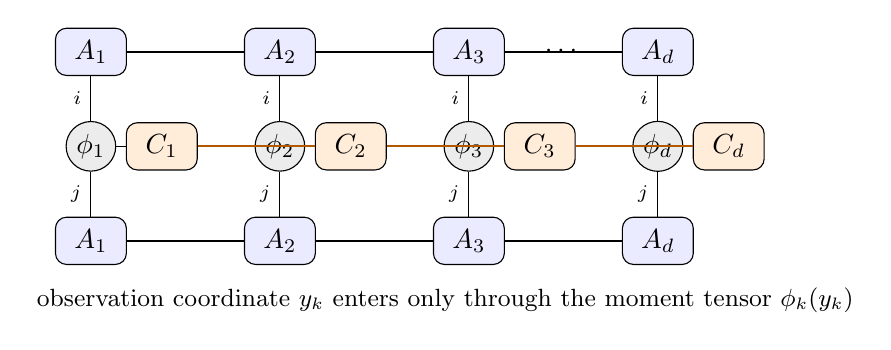
\begin{tikzpicture}[core/.style={draw,rounded corners,minimum width=9mm,minimum height=6mm,fill=blue!8},
  ker/.style={draw,rounded corners,minimum width=9mm,minimum height=6mm,fill=orange!15},
  mom/.style={draw,circle,inner sep=1.5pt,fill=gray!15}]
\foreach \k/\lab in {0/1,1/2,2/3,3/d}{
  \node[core] (g\k) at (2.4*\k,1.2) {$A_{\lab}$};
  \node[core] (h\k) at (2.4*\k,-1.2) {$A_{\lab}$};
  \node[ker] (u\k) at (2.4*\k+0.9,0) {$C_{\lab}$};
  \node[mom] (m\k) at (2.4*\k,0) {$\phi_{\lab}$};
  \draw (g\k) -- node[left,font=\scriptsize]{$i$} (m\k);
  \draw (h\k) -- node[left,font=\scriptsize]{$j$} (m\k);
  \draw (u\k) -- (m\k);
}
\node[font=\small] at (4.5,-1.95) {observation coordinate $y_k$ enters only through the moment tensor $\phi_k(y_k)$};
\foreach \k/\l in {0/1,1/2,2/3}{
  \draw[thick] (g\k) -- (g\l); \draw[thick] (h\k) -- (h\l); \draw[thick,orange!70!black] (u\k) -- (u\l);}
\node at (6.0,1.2) {$\cdots$};
\end{tikzpicture}
\caption{Tensor network for $Z\,q(y)$ in~\eqref{eq:qcontract}. Two copies of the amplitude TT (blue) and the noise TT
(orange) meet at the per-axis moment tensors $\phi_k(y_k)$. These are exact polynomials in $y_k$, precomputed once.
The contraction proceeds left to right with an $r\times r\times s$ state.}
\label{fig:network}
\end{figure}

\begin{remark}[What is and is not exact]
The only approximation in the likelihood is the representation of the prescribed noise by the Chebyshev TT
$U$ on the window $W$. That representation is checked against the analytic kernel (to $10^{-9}$ of its peak for
the kernels used here) and can be made as accurate as desired by adding modes. In particular there is no sampling of
the noise and no approximation of $g^2$ by a lower-rank TT. Chebyshev approximations of Gaussians can have
tiny negative tails. Plots clip these, and the clipped mass is recorded and required to be below $10^{-5}$.
\end{remark}

%======================================================================
\section{Regularization}
\label{sec:reg}

\subsection{Amplitude Sobolev seminorms}
\label{sec:sobolev}
For $s\in\{1,2\}$ and length scales $\ell_k>0$ define
\begin{equation}\label{eq:sobolev}
  R_s(\mathcal A)=\sum_{k=1}^d \ell_k^{2s}\,\frac{\norm{\partial_k^s g_{\mathcal A}}_{L^2(\Omega)}^2}{\norm{g_{\mathcal A}}_{L^2(\Omega)}^2}.
\end{equation}
It is invariant under gauge, scale and sign, since it depends only on $p_{\mathcal A}$. For $s=1$,
\begin{equation}
  \frac{\norm{\partial_k g}^2}{\norm g^2}=\int\bigl(\partial_k\sqrt{p}\bigr)^2=\frac14\int\frac{(\partial_kp)^2}{p},
\end{equation}
one quarter of the location Fisher information of $p$ along axis $k$. So $R_1$ penalizes exactly the quantity that a
noisy likelihood cannot see well. The numerator is computed exactly by replacing $M_k$ with the derivative Gram
matrix $D^{(s)}_k=\Delta_k^sM_k(\Delta_k^s)^\T$ in one factor of the transfer recursion, where $\Delta_k$ is the Chebyshev
differentiation matrix scaled by $2/(b_k-a_k)$. With $(N_k,E_k)$ the running (numerator, norm) states,
$N_k=\mathcal E_k(N_{k-1})+\ell_k^{2s}\mathcal D_k(E_{k-1})$ and $E_k=\mathcal E_k(E_{k-1})$. In deconvolution we take
$\ell_k$ to be the standard deviation of the $k$-th univariate marginal of $U$, computed from the noise TT itself,
and use $s=2$ (``amplitude $H^2$''). Mixed derivatives are omitted.

\subsection{Marginal Fisher-visibility filter}
\label{sec:fisher}
The Sobolev penalty damps every high-frequency direction equally. The \emph{visibility filter} instead damps
the directions the noise actually hides. Fix an axis $k$, a reference marginal density $\rho$ on $[a_k,b_k]$
(the \emph{pilot}, \S\ref{sec:pilot}), and the univariate noise marginal $u$ of $U$. Consider amplitude
perturbations $\sqrt\rho\mapsto\sqrt\rho+th$ with $h\perp\sqrt\rho$ in $L^2$ and $\norm h=1$. The complete-data
Fisher information of $t$, divided by four, equals $\norm h^2=1$. The \emph{observed} (noisy) one is
\begin{equation}\label{eq:fisher}
  \mathcal F(h,h)=\int\frac{\bigl(u*(\sqrt\rho\,h)\bigr)^2}{u*\rho}\dd y\in[0,1],
\end{equation}
after projecting out the normalization direction. It lies in $[0,1]$ because the noisy score is a conditional
expectation of the clean score. Discretize $h$ in the $L^2$-orthonormal Chebyshev basis restricted to
$\sqrt\rho^{\perp}$, and diagonalize $\mathcal F=\sum_m\lambda_mv_mv_m^\T$. With a visibility floor $\alpha>0$ the
per-axis penalty operator is
\begin{equation}\label{eq:filter}
  P_k=\sum_m\frac{\alpha}{\alpha+\lambda_m}\,v_mv_m^\T\qquad\text{(and }P_k\sqrt\rho=0\text{)},
\end{equation}
mapped back to Chebyshev coefficients. The functional $R_F(\mathcal A)=\sum_k\ip{g}{(P_k)_{\text{axis }k}\,g}/\norm g^2$
is computed by the same two-state recursion as $R_s$, with $P_k$ in place of $D_k^{(s)}$. Nearly invisible directions
($\lambda\ll\alpha$) receive weight $\approx 1$, well-observed ones ($\lambda\gg\alpha$) weight $\approx\alpha/\lambda$, and
the reference itself is free. The full correlated $U$ still enters the likelihood. Only the regularizer uses
marginal geometry, and it needs no Gaussian assumption on $U$.

\subsection{Pilot marginals}
\label{sec:pilot}
Pilots are exponential-family marginals $\log\rho_k=\sum_{j=1}^{m}\theta_{kj}T_j\circ\tau_k$ with $m\in\{2,4,6,8\}$,
either shared across axes (in standardized coordinates) or separate. They are fitted by the binned noisy
marginal likelihood through the univariate noise marginal (L-BFGS, 1{,}600 bins, at most 1{,}200 iterations),
from a moment-corrected Gaussian start. Degree and sharing are chosen by the rule of \S\ref{sec:select}, with the
parameter count as the complexity.

%======================================================================
\section{Model selection from noisy observations}
\label{sec:select}

Let $\ell_c(y_v)$ be the held-out log density of candidate $c$ at validation point $y_v$ ($v=1,\dots,V$), and
$c^\star=\argmin_c\bigl(-\frac1V\sum_v\ell_c(y_v)\bigr)$. For each $c$ form the paired excesses
$e_{cv}=\ell_{c^\star}(y_v)-\ell_c(y_v)$, their mean $\bar e_c$, and a cluster-robust standard error $\mathrm{SE}_c$
(clusters are MCMC chains for Ginzburg--Landau, single observations otherwise). The eligible set is
$\{c:\bar e_c\le \mathrm{SE}_c\}$, and among eligible candidates we pick the one with the smallest value of a
\emph{common} roughness functional (the Fisher penalty with a common filter, or $R_2$ with common length scales).
This is the one-standard-error rule~\cite{hastie2009elements} applied to paired differences. It is a heuristic,
not a post-selection confidence statement, and the same validation split is reused across stages. As the
experiments show (\S\ref{sec:swirl}), it is also the weakest link. Candidates that differ visibly in the latent
density can be indistinguishable in noisy NLL.

%======================================================================
\section{The two recipes}
\label{sec:recipes}

\begin{algorithm}[H]
\caption{Gallery recipe for Ginzburg--Landau (\texttt{scripts/refresh\_density\_fits.py})}
\label{alg:gl}
\begin{algorithmic}[1]
\STATE Latent box: training min/max $+10\%$ (noise-free) or noisy $0.5$--$99.5\%$ quantiles $+5\%$ (noisy).
\STATE LSCV bandwidth; TT-qTensGE of $\sqrt{\mathrm{KDE}}$ at rank $r$ ($8$ for $d\le 8$, $10$ for noisy or $d\le14$, else $14$), 21 (noise-free) or 25 (noisy) modes, 64 starts.
\IF{noise-free}
  \STATE Adam on~\eqref{eq:nll}, 8{,}000 steps, lr $10^{-3}$, batch 2048; checkpoint by validation NLL.
\ELSE
  \STATE Warm-up: Adam on noisy NLL $+\;3\cdot10^{-5}R_2$, 8{,}000 steps, lr $5\cdot10^{-4}$, batch 256.
  \STATE Pilots $\rho_k$ (degrees 2--8, shared/separate) selected by the paired one-SE rule.
  \STATE Pad to 33 modes (more if the pilot amplitude is under-resolved); build $R_F$ with $\alpha=0.01$.
  \STATE For $\lambda\in\{0.1,0.3,1\}$: continue from the warm-up on noisy NLL $+\lambda R_F$, 8{,}000 steps.
  \STATE Select among warm-up and the three Fisher fits: paired one-SE, then minimum common $R_F$.
\ENDIF
\end{algorithmic}
\end{algorithm}

\begin{algorithm}[H]
\caption{High-capacity recipe for cryo-EM and swirl--pretzel (\texttt{refine\_cryoem\_continuity.py}, \texttt{swirl\_fits.py})}
\label{alg:hi}
\begin{algorithmic}[1]
\STATE Base fit as in Algorithm~\ref{alg:gl} (init rank 16 for swirl), without the Fisher stage.
\STATE For $r\in\{32,64\}$: continue at 49 modes (\S3.3). Noisy: $\lambda\in\{10^{-4},3\cdot10^{-4}\}$ times $R_2$, Sobolev preconditioning, 3{,}200 steps, lr $2\cdot10^{-4}$, batch 256, checkpoints by validation NLL $+\lambda R_2$.
\STATE Noise-free: minimum validation NLL. Noisy: paired one-SE, then minimum common $R_2$.
\end{algorithmic}
\end{algorithm}

For rank~64 the backward pass of~\eqref{eq:qcontract} is memory-bound: one intermediate has
$B\cdot r^2 s\,n$ entries. The same 256-row minibatch gradient is therefore accumulated over four chunks, which gives an
identical gradient.

%======================================================================
\section{Experiments}
\label{sec:experiments}

All experiments use one GPU (NVIDIA A100 or H100). Truth, clean samples and state labels enter only after fitting and selection. The
error $\relLtwo$ is always full-dimensional. For Ginzburg--Landau, $\int\hat p^2$ is Gauss--Legendre quadrature of
the degree-$4(n-1)$ amplitude polynomial, and $\int p\hat p$ and $\int p^2$ come from the transfer-operator
recursion of the chain. For the swirl--pretzel density they are path quadratures (\S\ref{sec:swirl}). Every quadrature is
refined until it changes by less than $10^{-7}$ relative.

\subsection{Ginzburg--Landau}
\label{sec:gl}
The target is the discretized Ginzburg--Landau field of~\cite[Simulation IV]{peng2024vrs},
\[
  p(x)\propto\exp\Bigl(-\beta\Bigl[\sum_{i=0}^{d}\tfrac{\lambda}{2}\bigl(\tfrac{x_{i+1}-x_i}{h}\bigr)^2
  +\sum_{i=1}^{d}\tfrac1{4\lambda}(1-x_i^2)^2\Bigr]\Bigr),\quad x_0=x_{d+1}=0,\ \beta=\tfrac18,\ \lambda=0.02,\ h=\tfrac1{d+1}.
\]
It has double-well marginals coupled along a chain, so every pair marginal is a set of four blobs. Samples come
from 200 single-site Metropolis chains; there are 100{,}000 training and 2{,}048 validation samples. Two noise families
are scaled by $1.5$: a \emph{paired} Gaussian with standard deviation $0.83$ and correlation $0.5$ within
coordinate pairs, and an isotropic \emph{mixture} $0.7\,\mathcal N(0,0.45^2I)+0.3\,\mathcal N(0,1.35^2I)$. The noise
is comparable to the distance between the wells at $\pm1$. The recipe is Algorithm~\ref{alg:gl}.

\begin{table}[h]
\centering
\begin{tabular}{rccc}
\toprule
$d$ & noise-free & paired Gaussian noise & Gaussian-mixture noise \\
\midrule
6  & 0.081 & 0.095 & 0.131 \\
10 & 0.109 & 0.141 & 0.136 \\
14 & 0.132 & 0.231 & 0.169 \\
20 & 0.161 & 0.244 & 0.236 \\
\bottomrule
\end{tabular}
\caption{Ginzburg--Landau, $N=100{,}000$: $\relLtwo$ of the recovered latent density (Algorithm~\ref{alg:gl}).}
\label{tab:gl}
\end{table}

\begin{figure}[p]
\centering
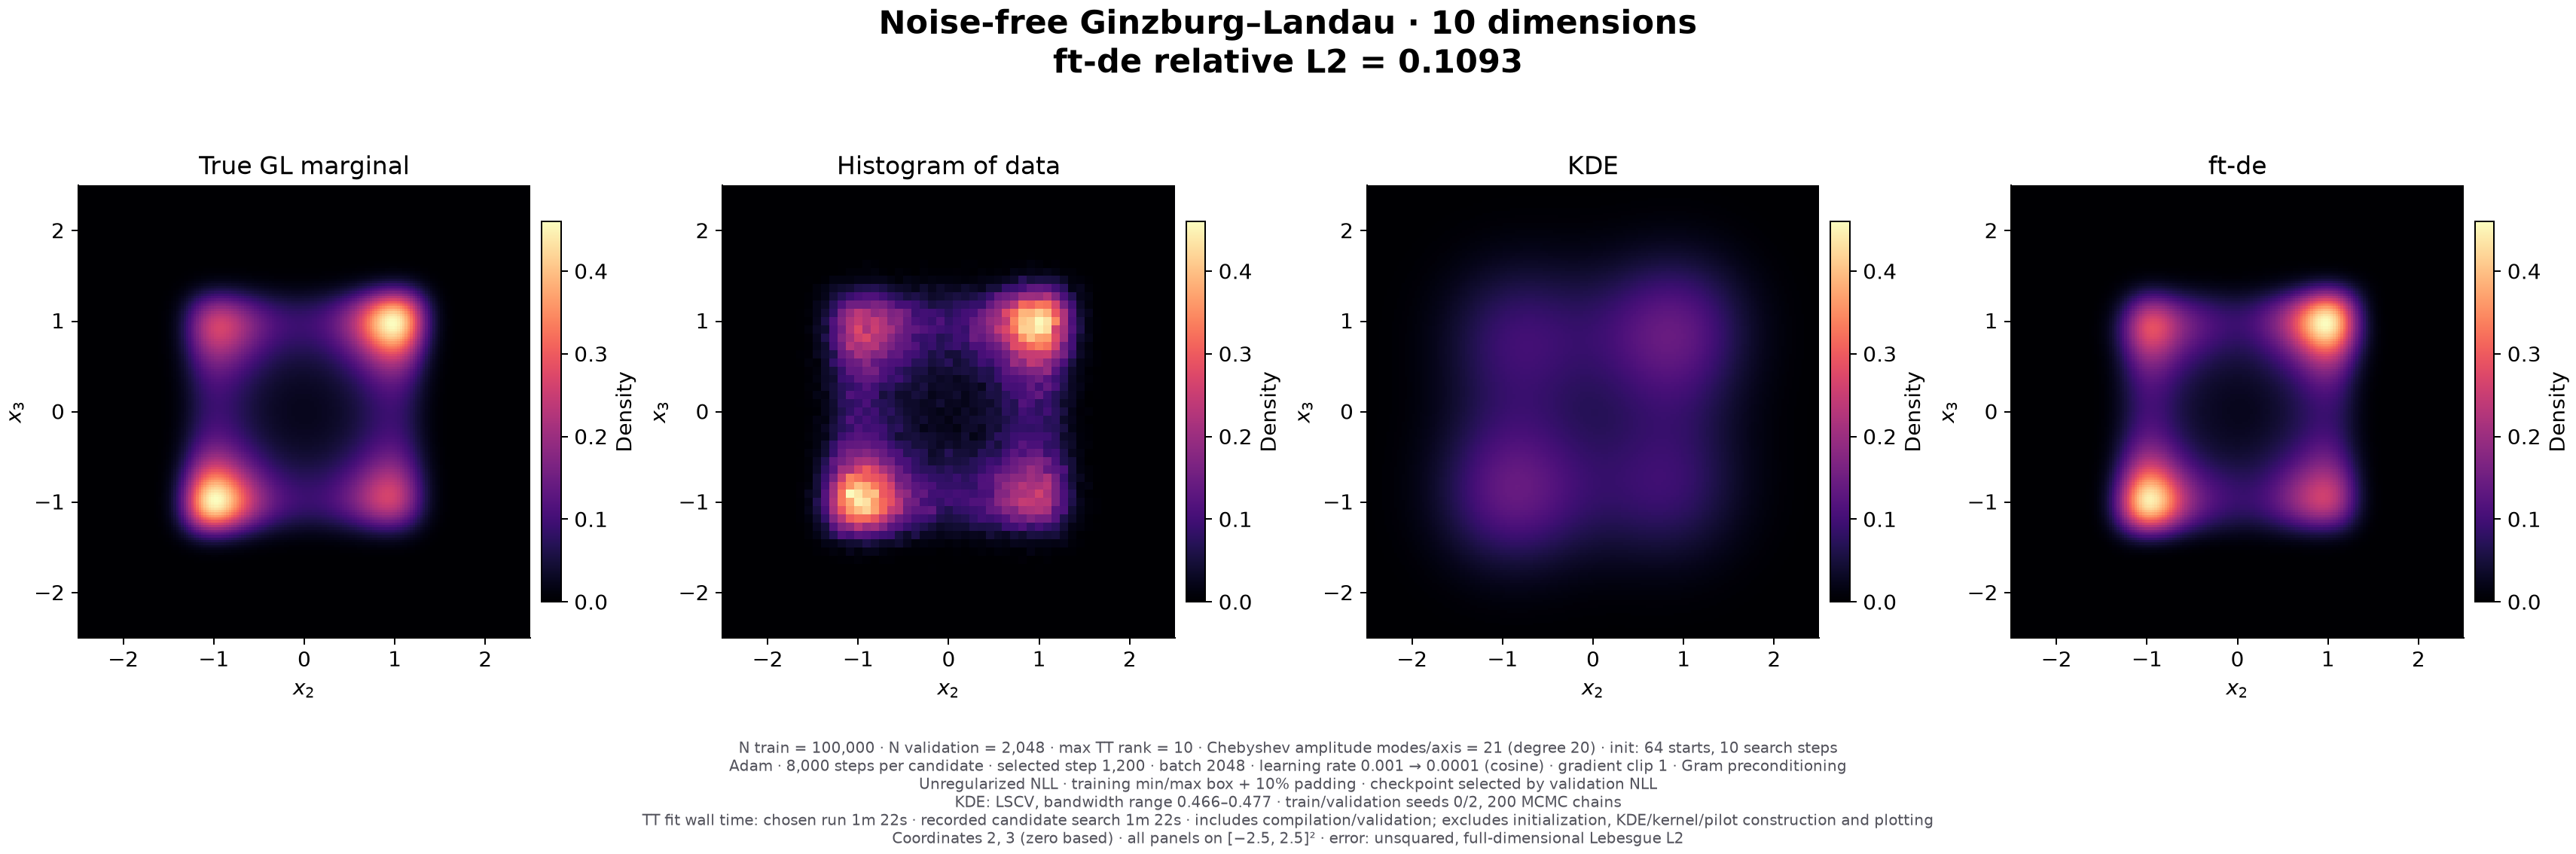
\includegraphics[width=\textwidth]{figures/gl_free_d10_23.png}\\[2mm]
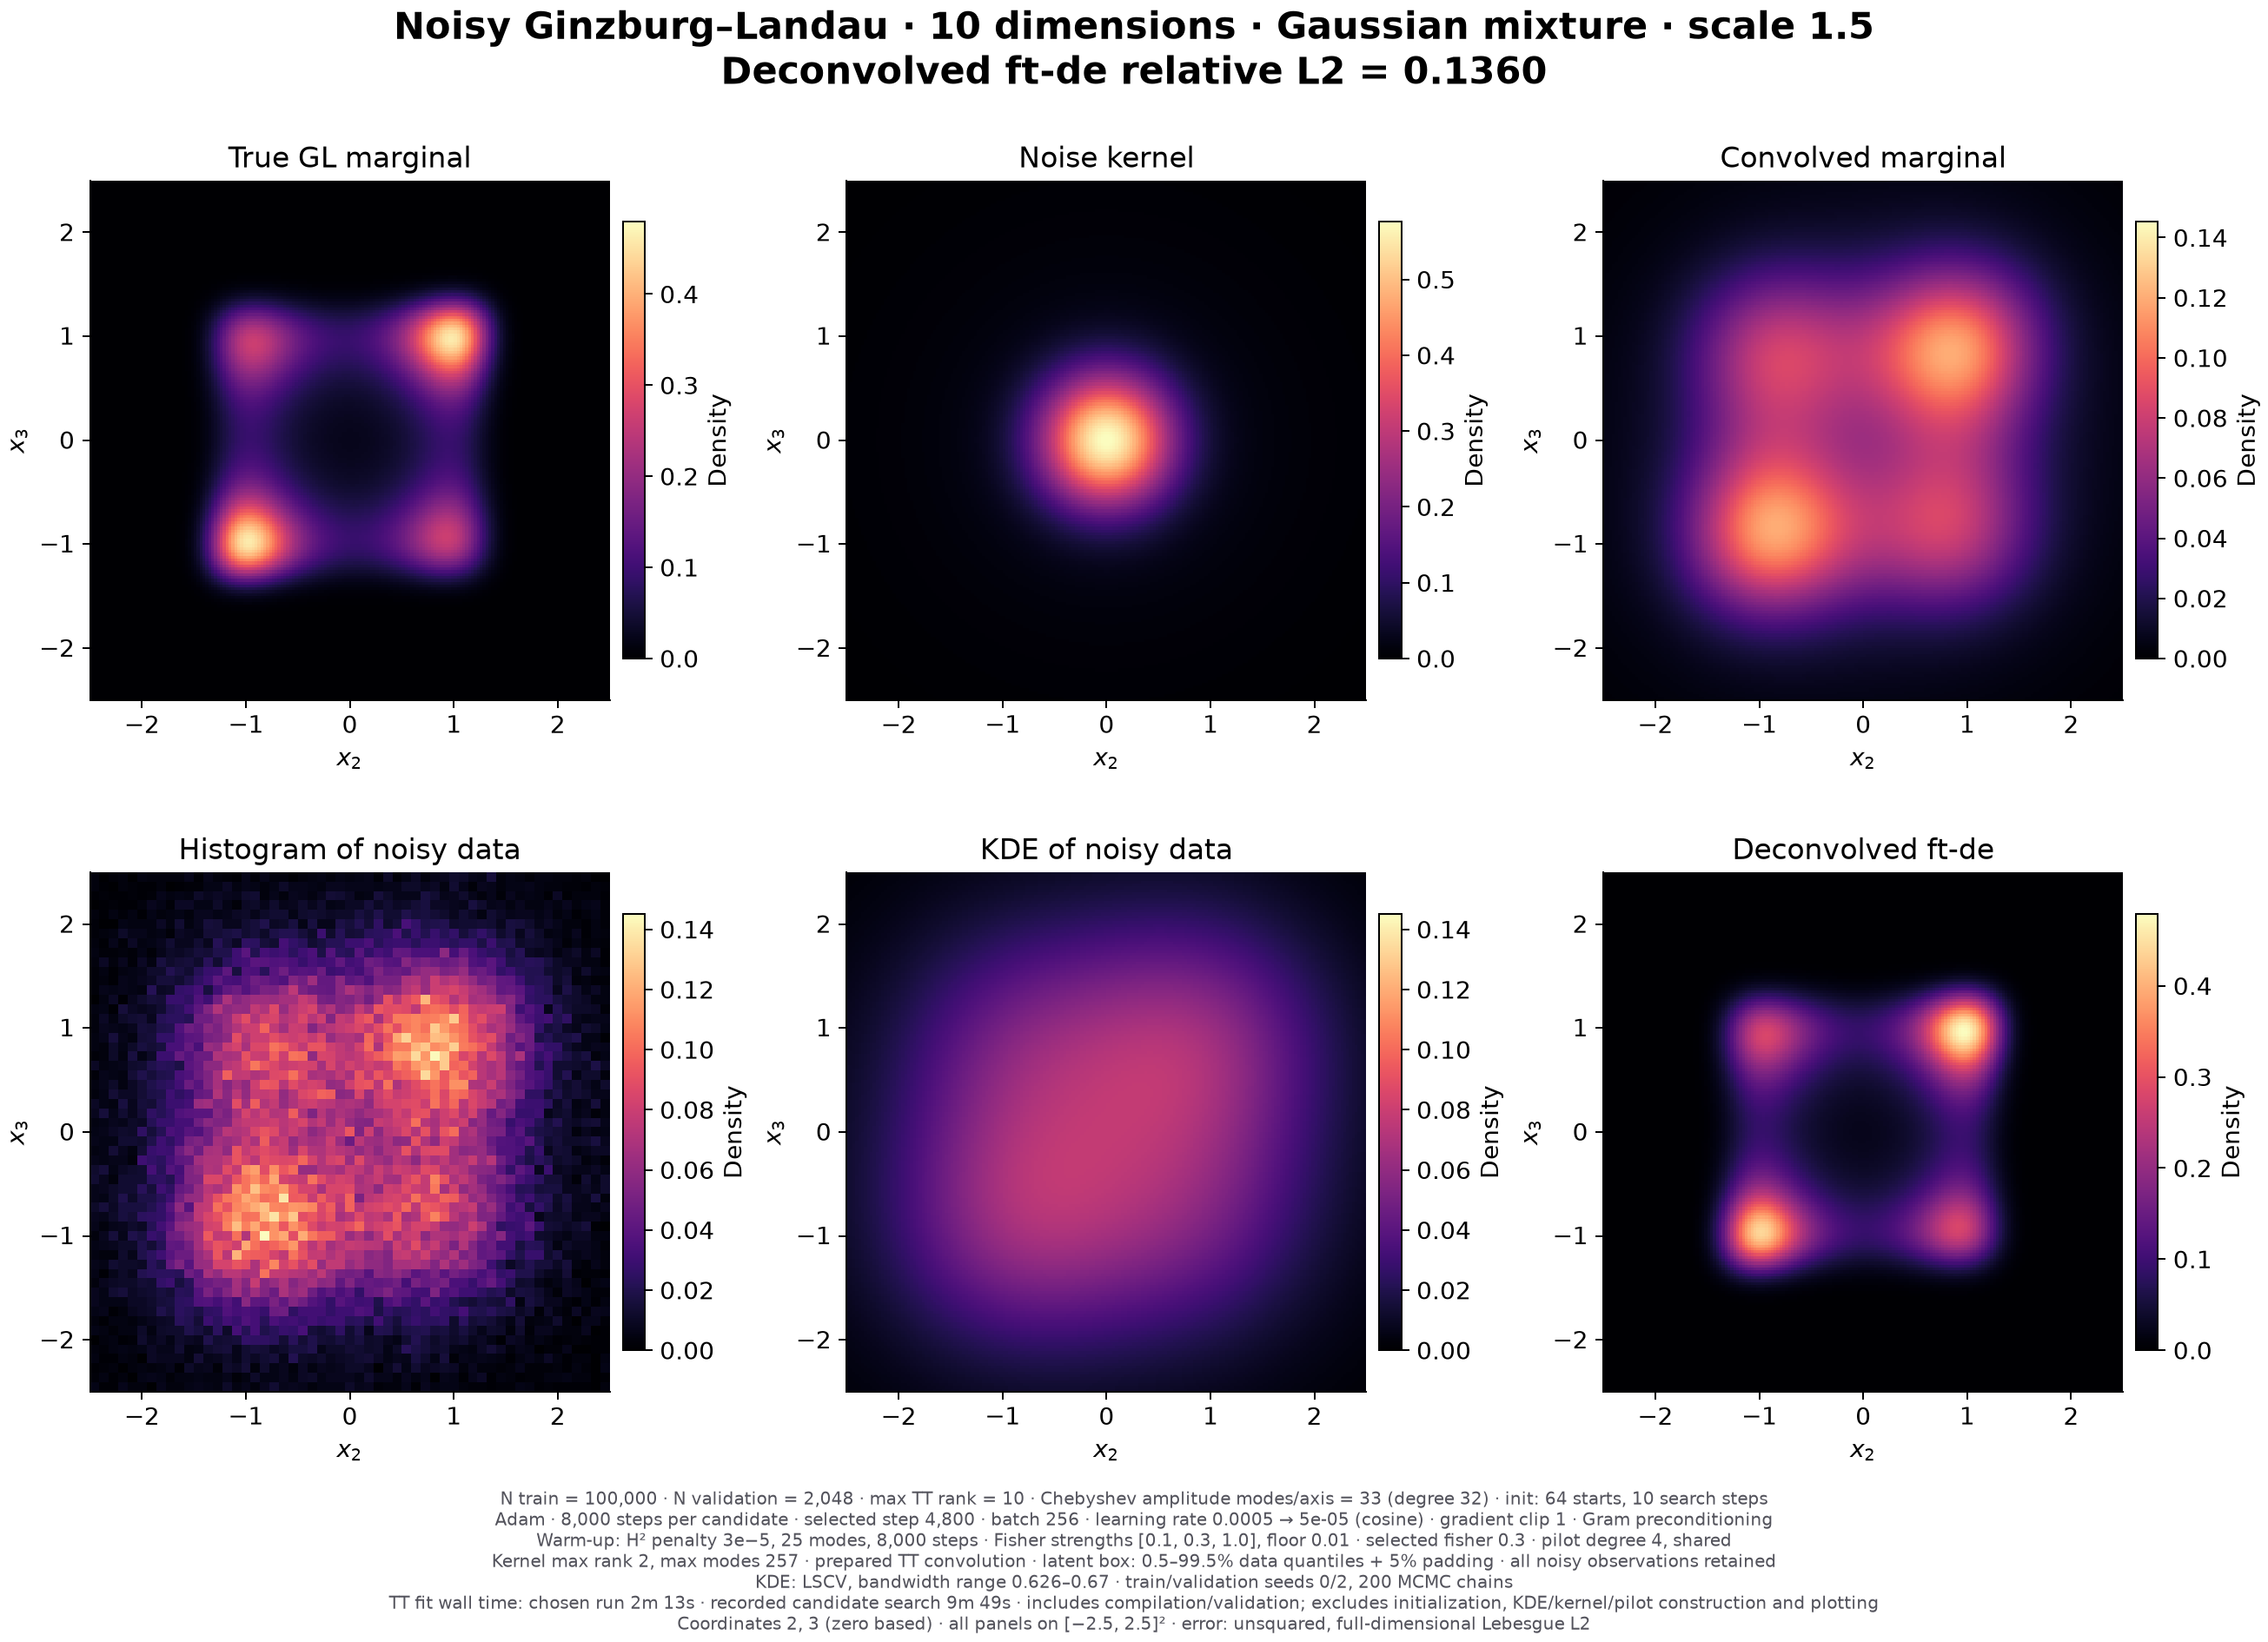
\includegraphics[width=.8\textwidth]{figures/gl_mix_d10_23.png}
\caption{Ginzburg--Landau, $d=10$, coordinates $(2,3)$. Top: noise-free (truth, training histogram, KDE, ft-de). Bottom:
mixture noise. Top row: truth, noise kernel, true convolved marginal. Bottom row: histogram and KDE of the noisy
data, and the deconvolved latent ft-de, with the same color scale as the truth. The recovered density separates the
four wells, including their unequal weights, although the noisy data show only two diffuse lobes.}
\label{fig:gl}
\end{figure}

\begin{figure}[t]
\centering
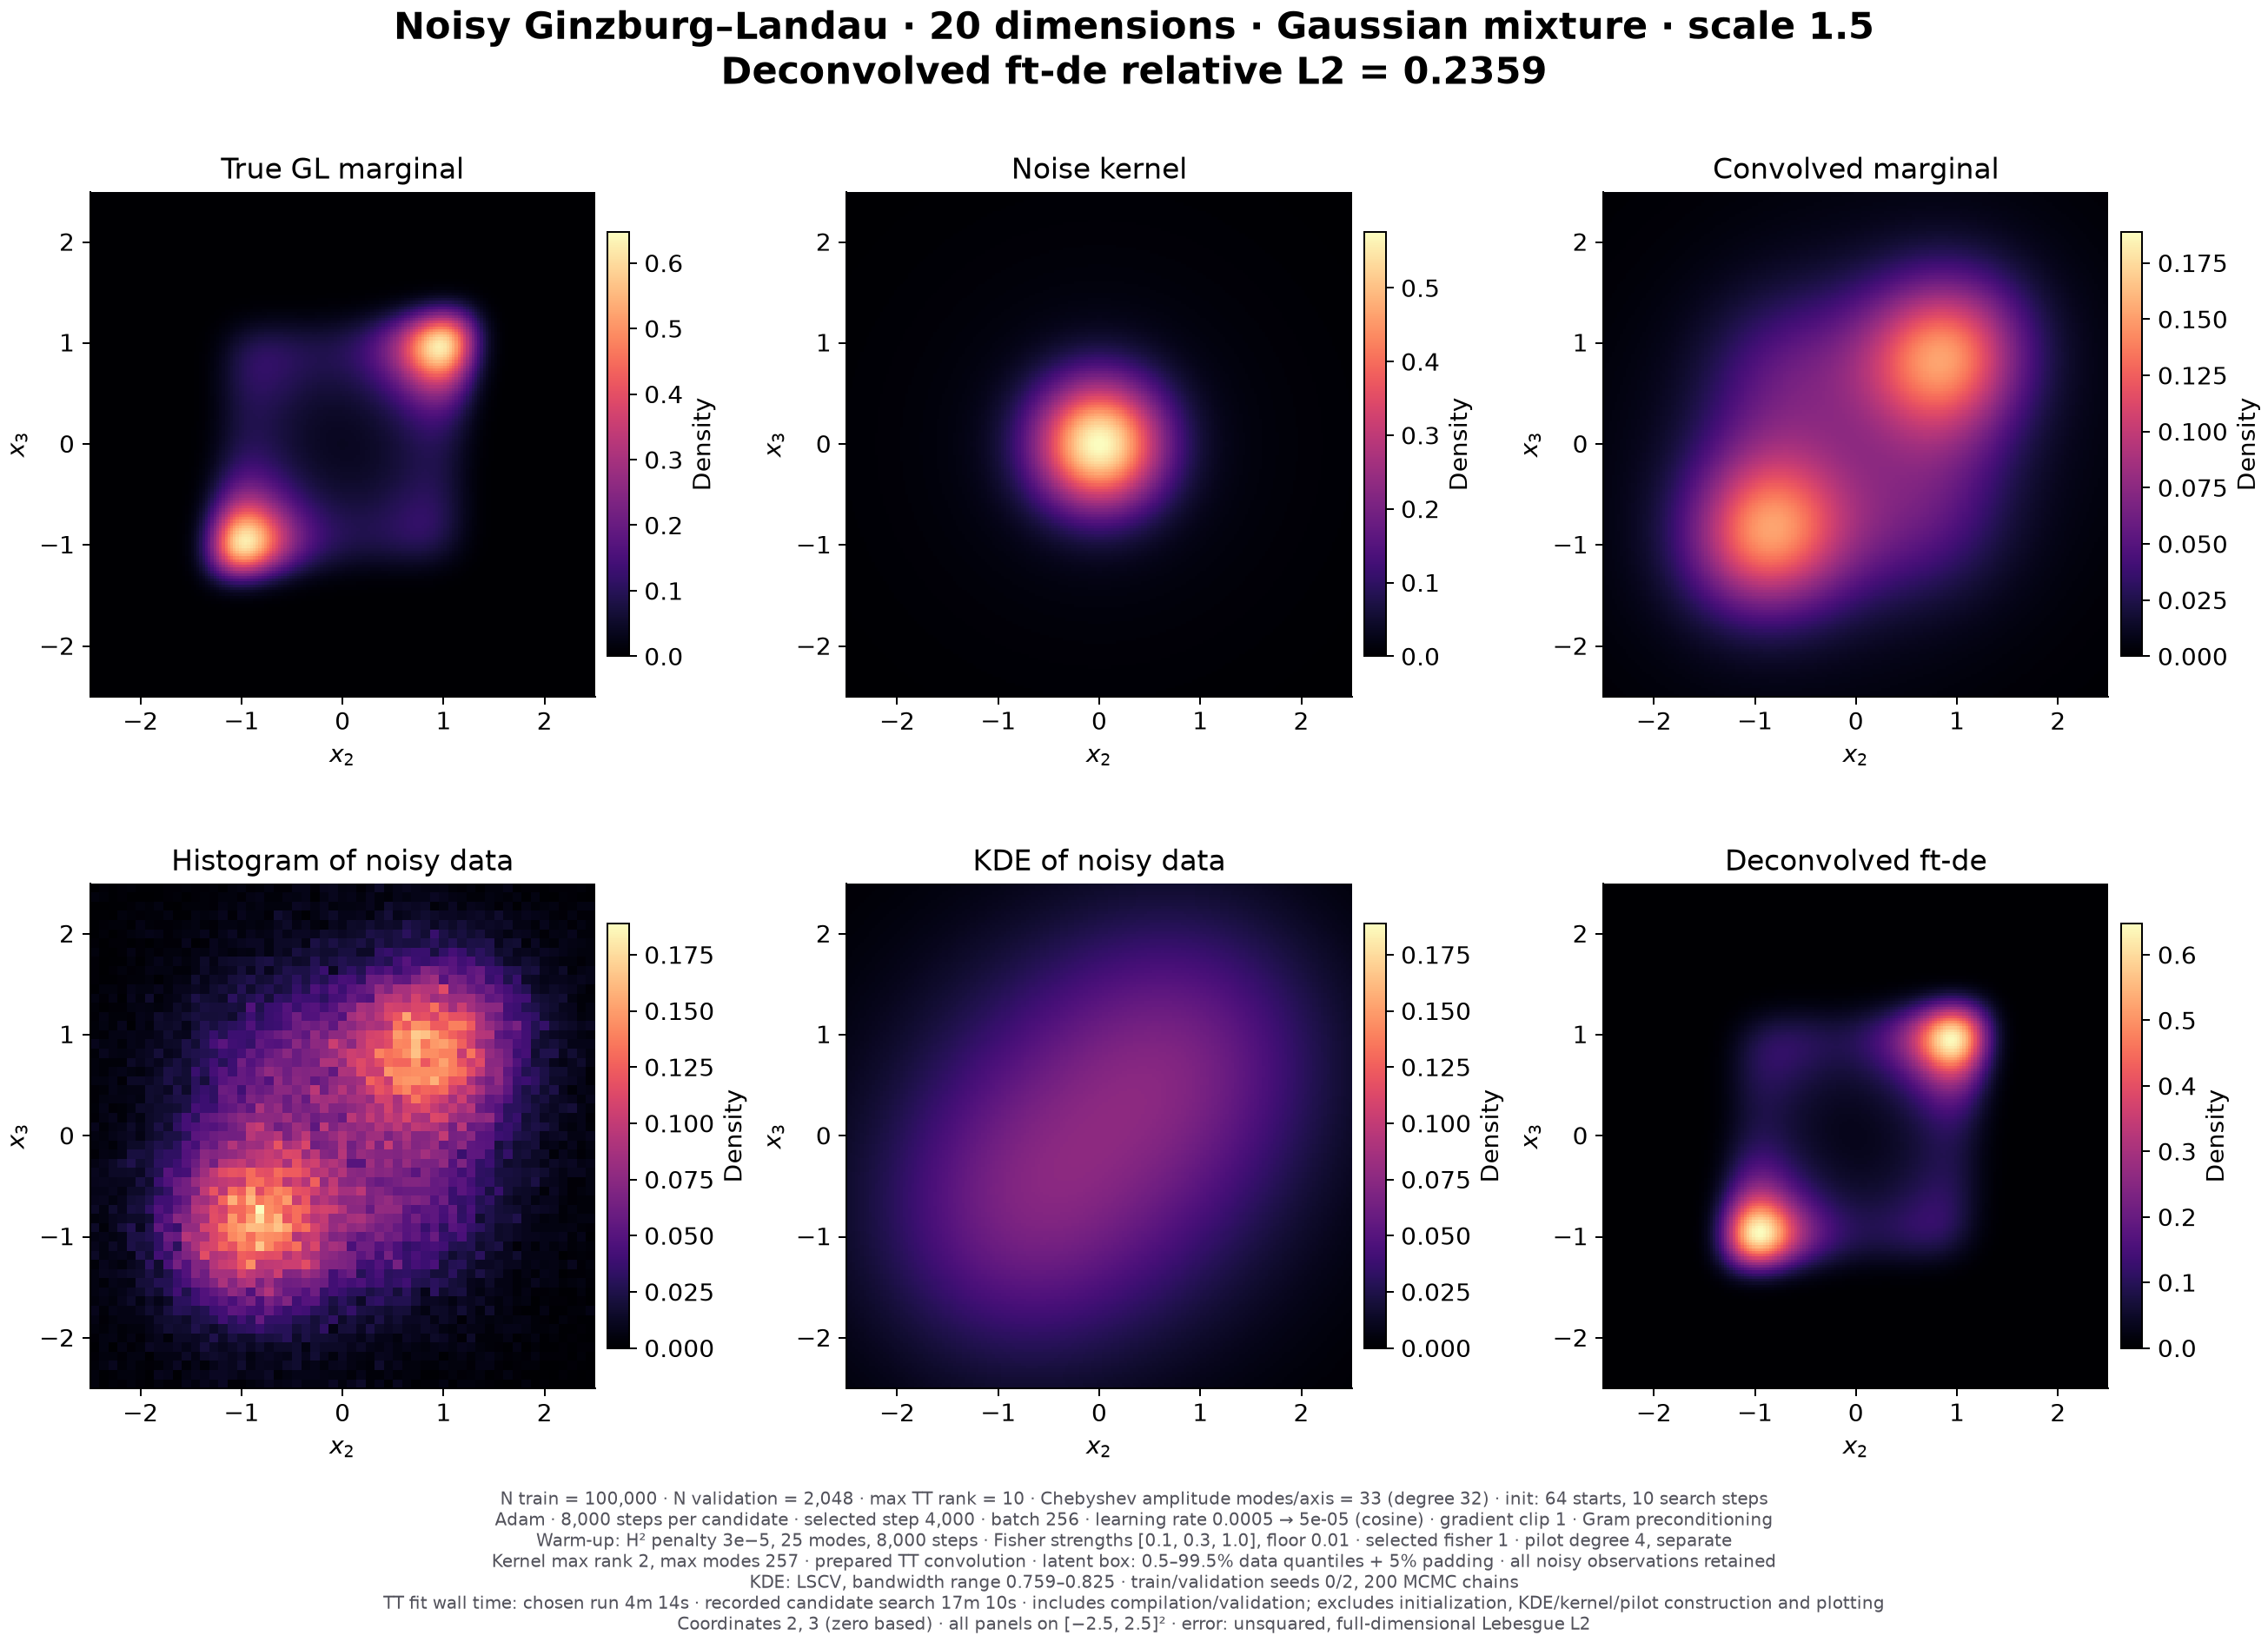
\includegraphics[width=.49\textwidth]{figures/gl_mix_d20_23.png}\hfill
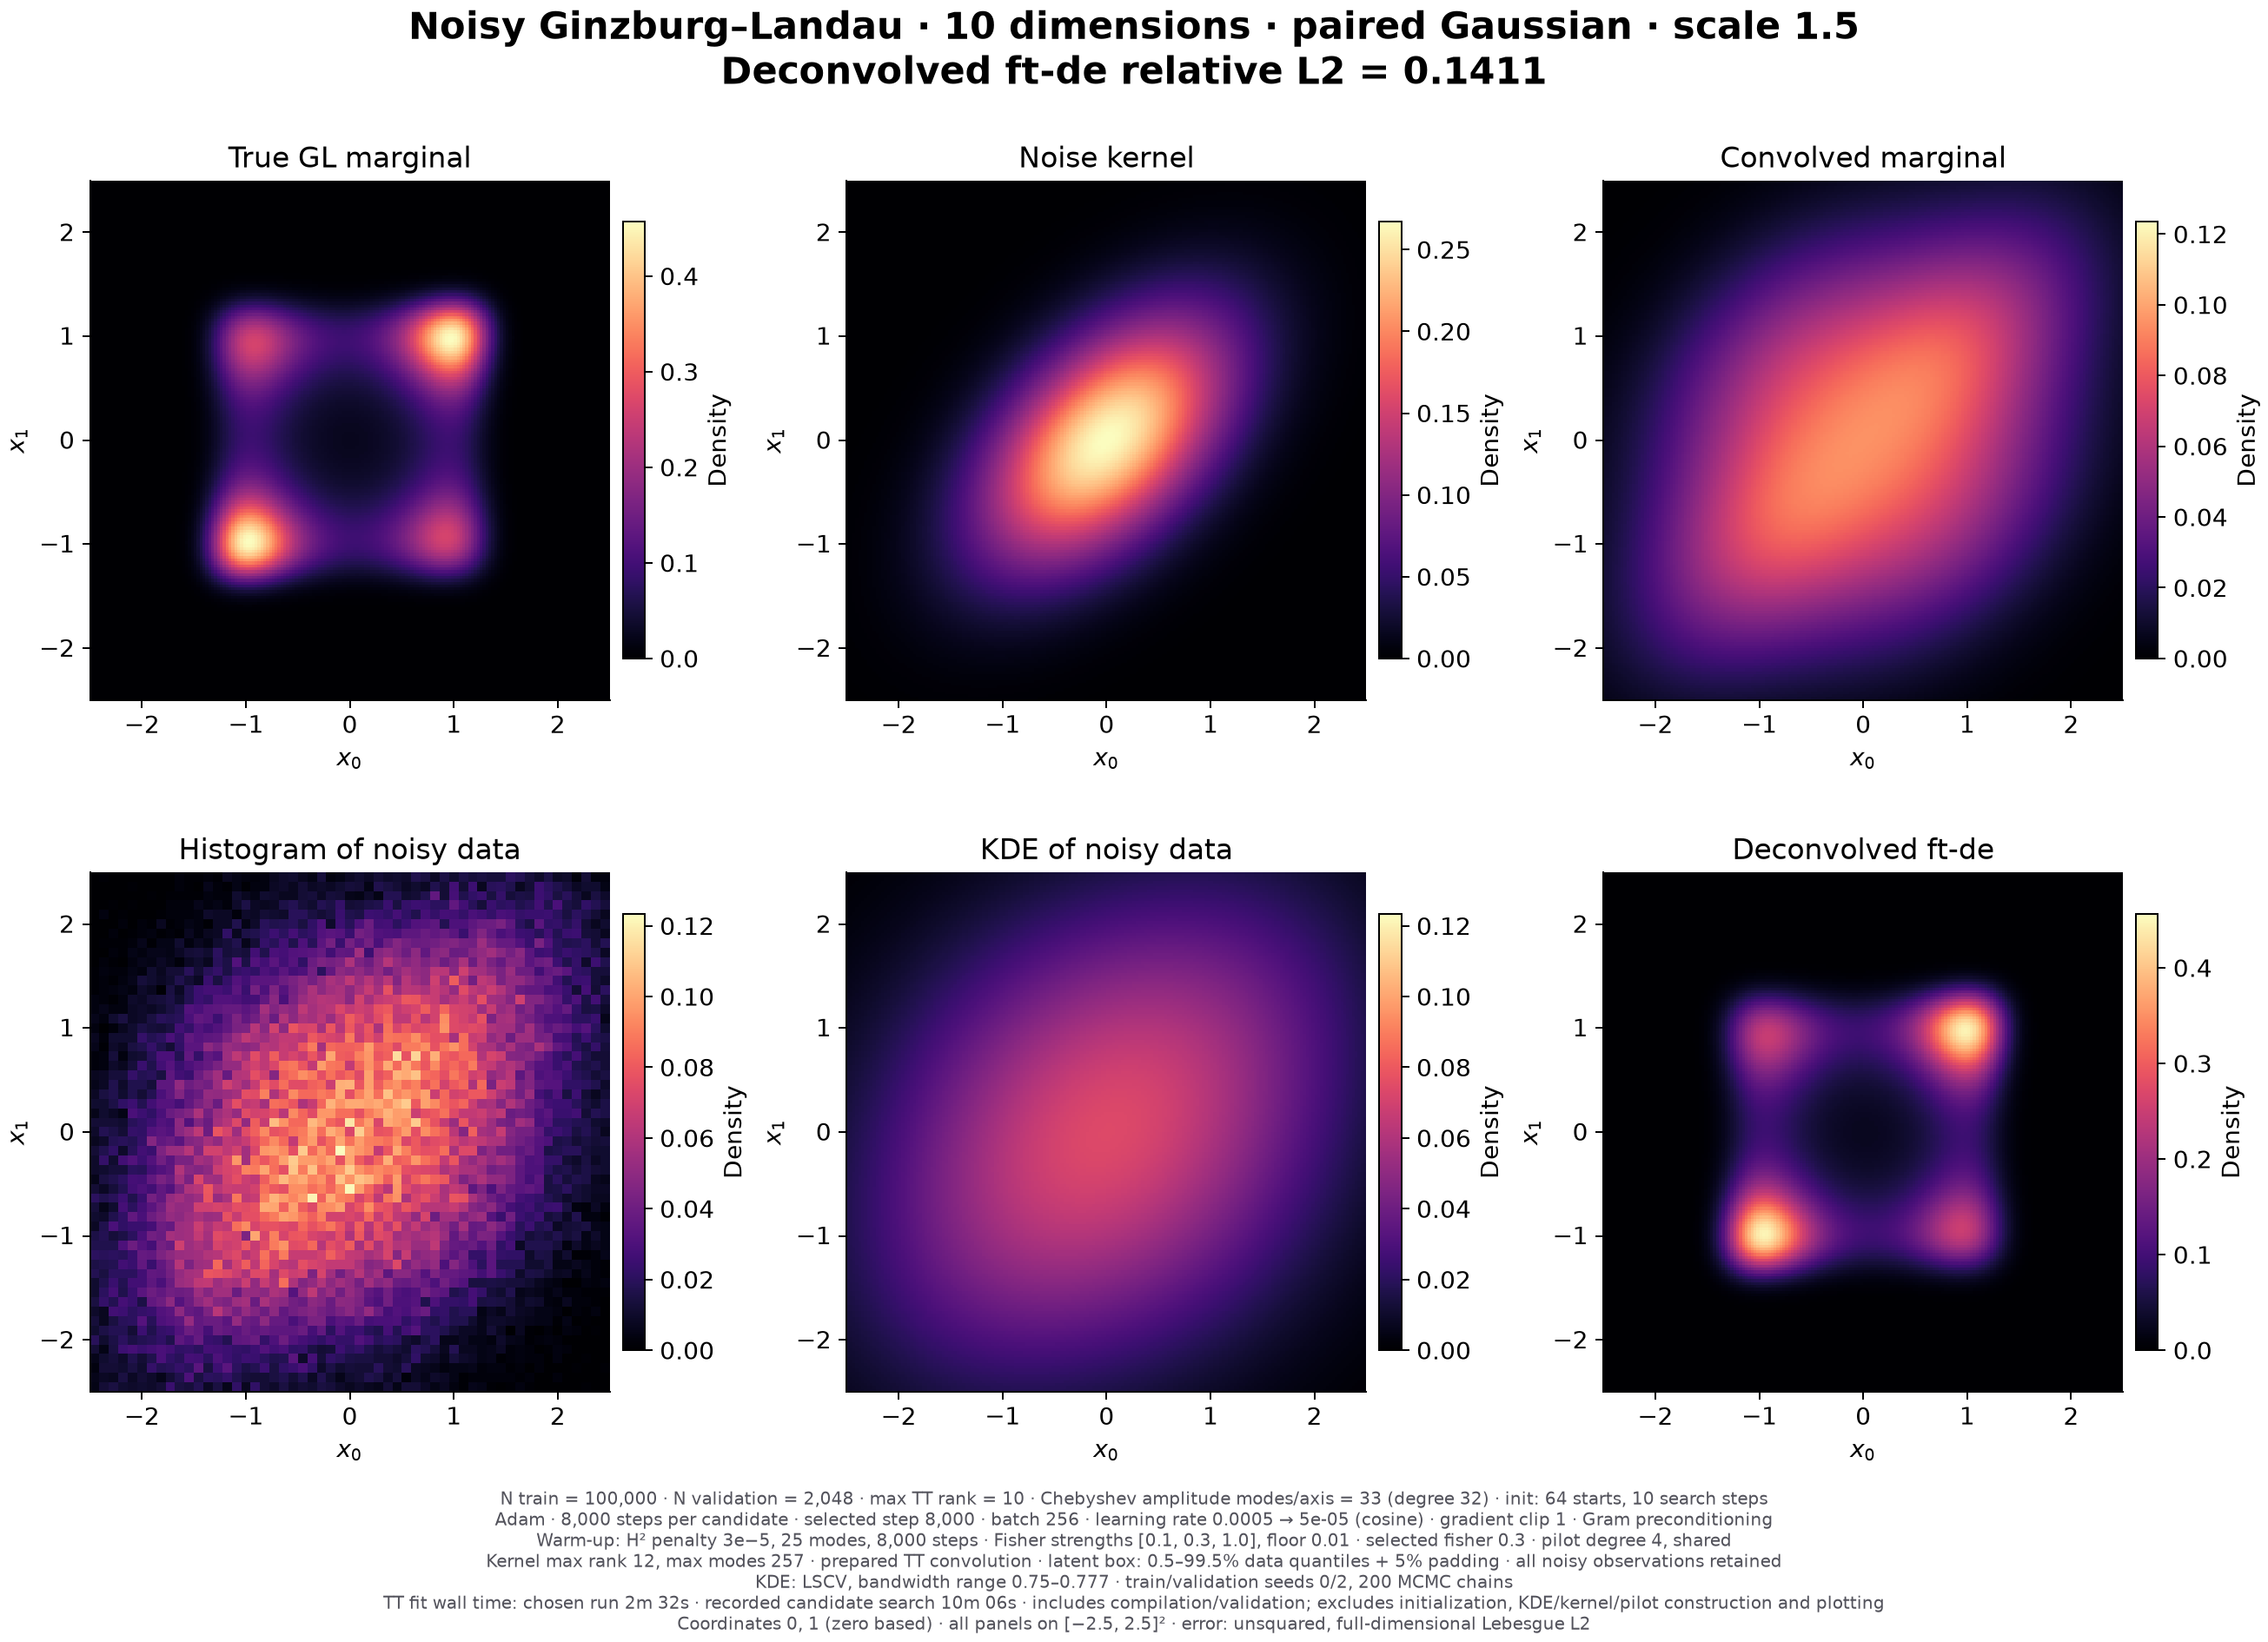
\includegraphics[width=.49\textwidth]{figures/gl_pair_d10_01.png}
\caption{Left: GL, $d=20$, mixture noise ($\relLtwo=0.236$). Right: $d=10$, correlated paired noise ($0.141$).}
\label{fig:gl2}
\end{figure}

The errors in Table~\ref{tab:gl} grow slowly with $d$. Figure~\ref{fig:gl} shows the qualitative behaviour: the deconvolved
estimate recovers four well-separated modes from data in which they are not visible. The GL density is close to
low rank and its pair marginals are nearly separable blobs. These are favourable conditions for a squared
Chebyshev TT, which is why we also test the harder geometry of \S\ref{sec:swirl}.

\paragraph{Fisher-visibility spectra.}
Figure~\ref{fig:fisher} shows the eigenvalues $\lambda_m$ of~\eqref{eq:fisher} for the $d=10$ mixture case. They decay
roughly geometrically, $\lambda\approx 0.63,0.18,0.07,0.02,0.007,\dots$, so on each axis only four or five amplitude
directions are observed above the floor $\alpha=0.01$. The filter leaves those almost free and damps the rest.

\begin{figure}[h]
\centering
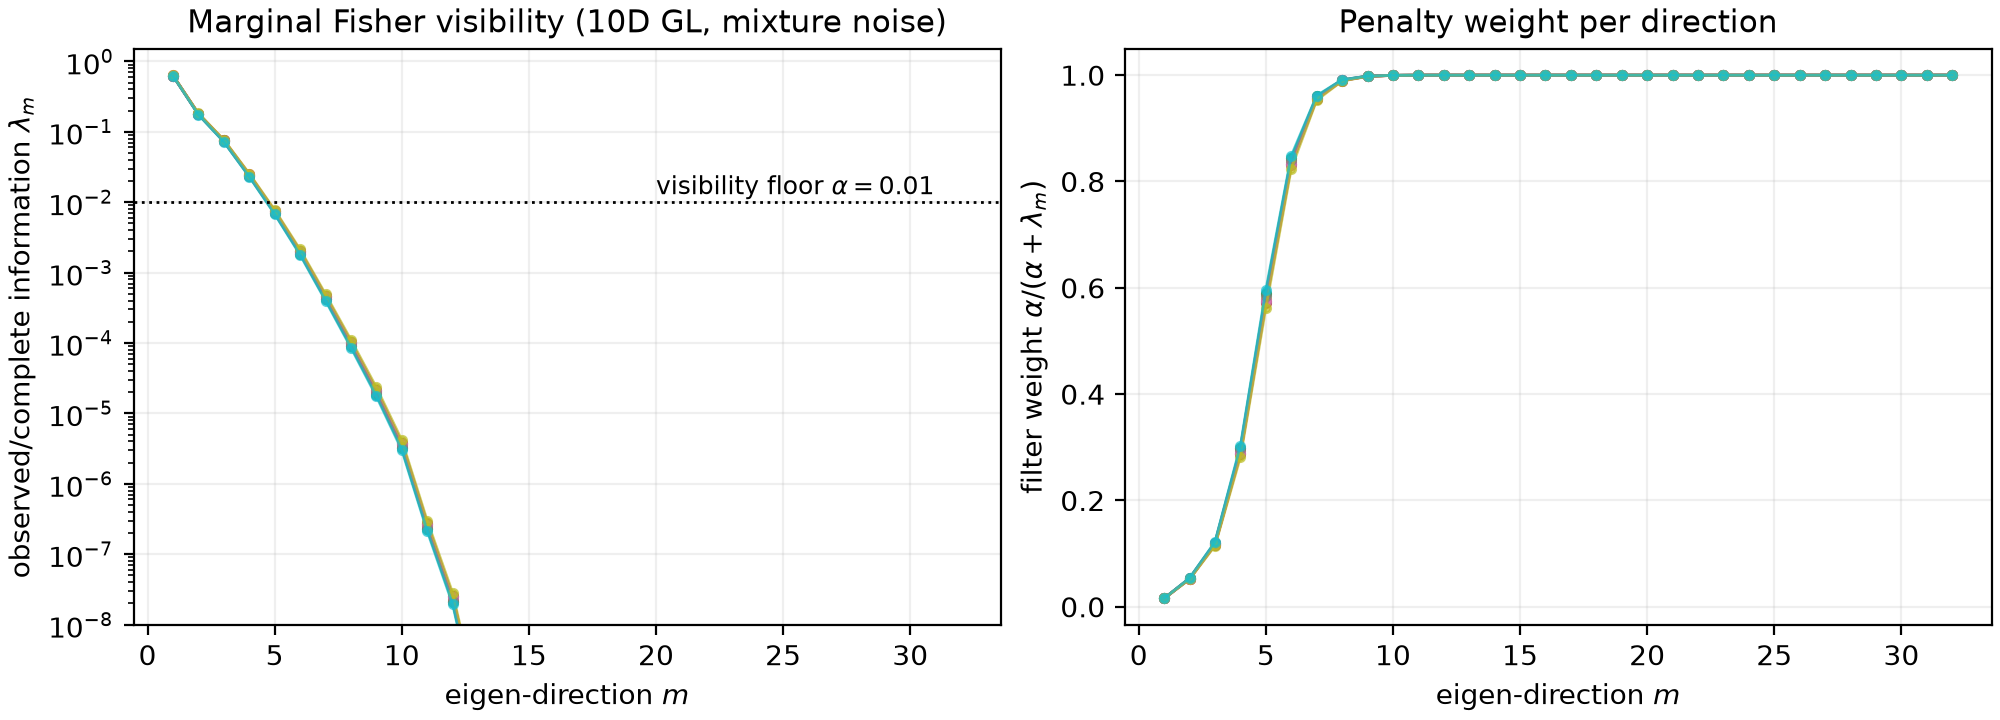
\includegraphics[width=.85\textwidth]{figures/fisher_spectrum.png}
\caption{Marginal Fisher-visibility eigenvalues~\eqref{eq:fisher} (one curve per axis) and the resulting penalty
weights~\eqref{eq:filter}, GL $d=10$ with mixture noise.}
\label{fig:fisher}
\end{figure}

\subsection{Sample-size convergence}
\label{sec:convergence}
To measure the finite-$N$ behaviour we reran the recipes \emph{unchanged} for
$N\in\{10^3,3\cdot10^3,10^4,3\cdot10^4,10^5,3\cdot10^5\}$: GL in $d=10$, noise-free and with mixture noise
(Algorithm~\ref{alg:gl}, training seeds 0 and 1), and the swirl--pretzel in $d=4$, noise-free and noisy
(Algorithm~\ref{alg:hi} with rank-32 continuations only, one seed). Rank, degree, step counts and penalty grids do
not depend on $N$, and the validation sets are fixed (2{,}048 GL and 4{,}096 swirl observations), so this measures
the recipe as used, not an estimator tuned to each $N$. The baseline is a Gaussian KDE whose LSCV bandwidth is
rescaled with Scott's exponent $N^{-1/(d+4)}$. In the noisy cases it is the KDE of the \emph{noisy} observations. It
estimates $q$, not $p$, so it shows what is lost without deconvolution. All errors are full-dimensional $\relLtwo$
against the clean latent density (for the GL KDE, $\int p\,\widehat{p}_{\rm KDE}$ is a Monte Carlo estimate over 200{,}000 exact
samples, with standard error below $10^{-3}$).

\begin{figure}[t]
\centering
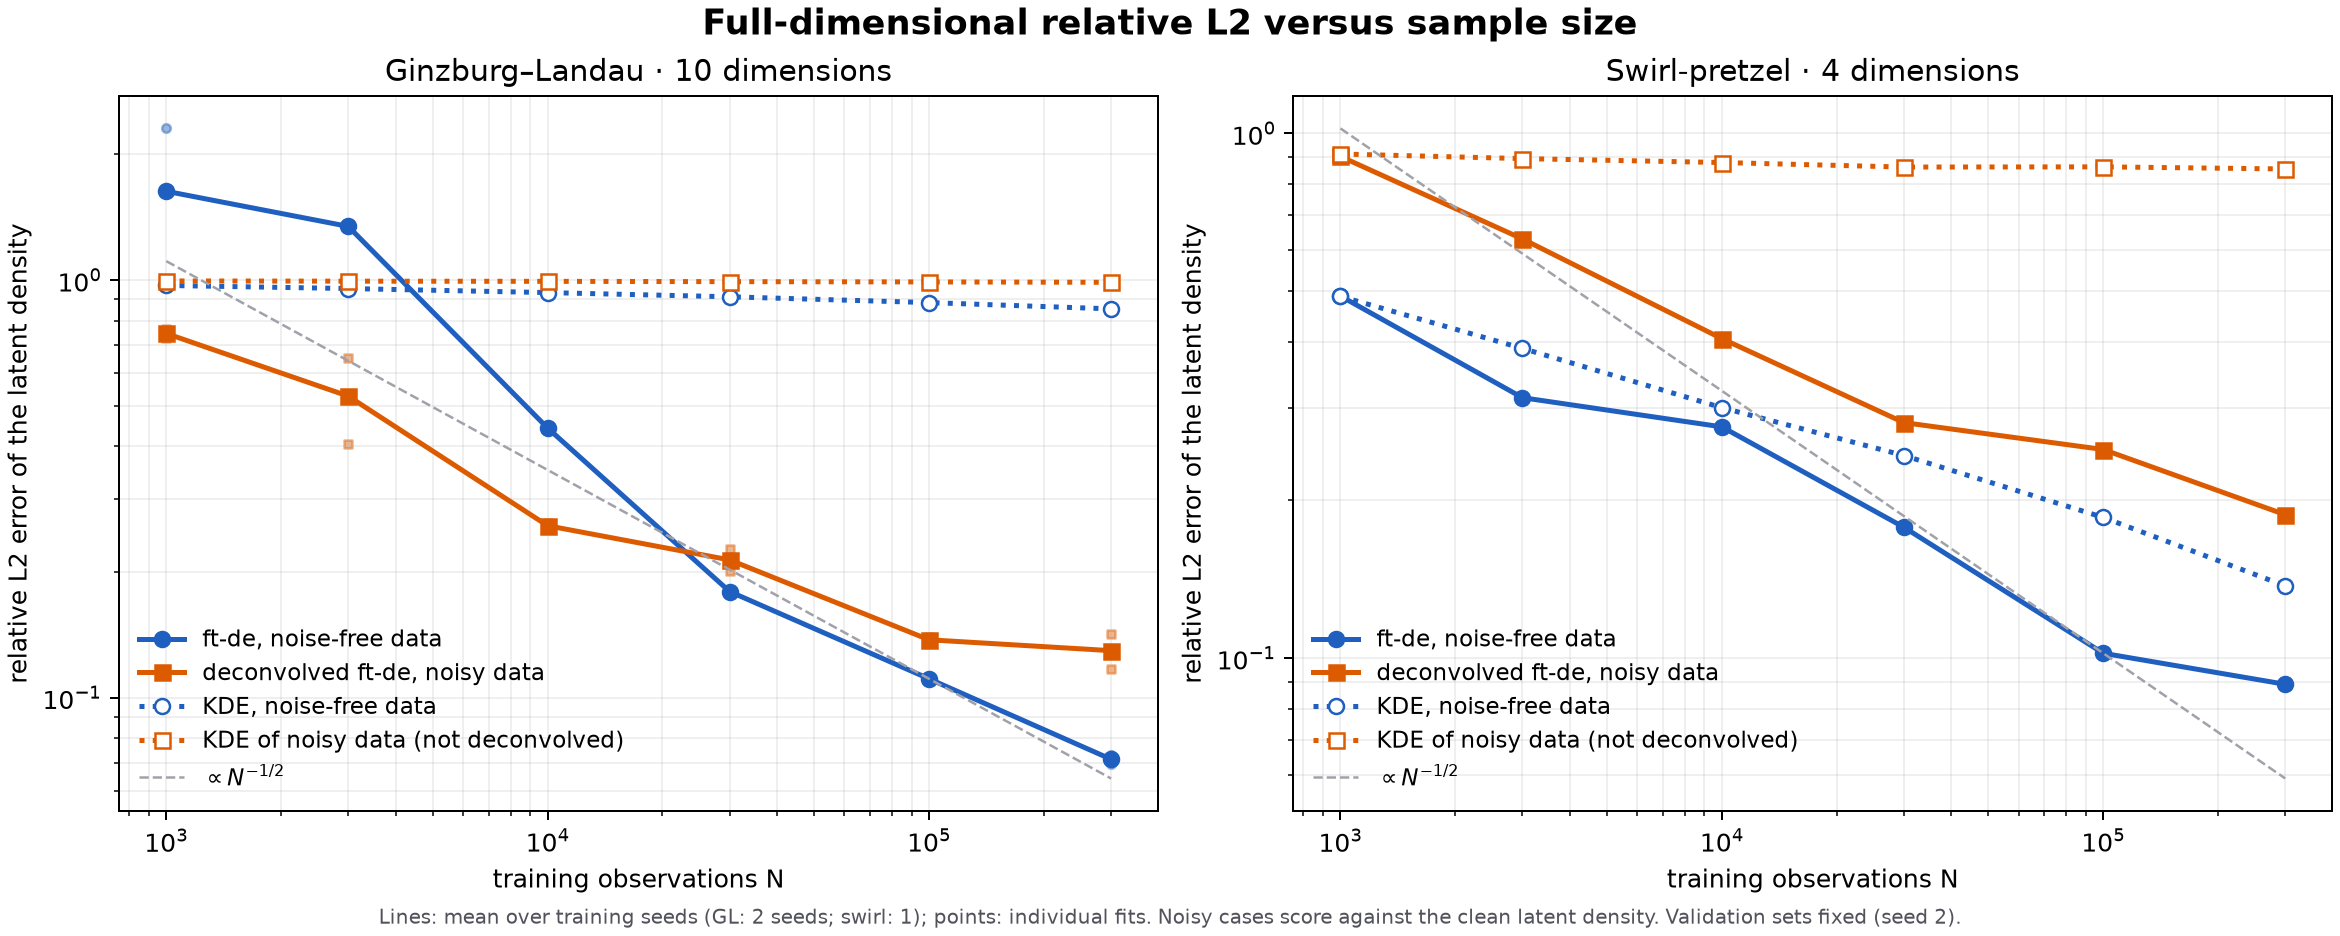
\includegraphics[width=\textwidth]{figures/convergence.png}
\caption{Full-dimensional $\relLtwo$ of the latent density against the number of training observations (log--log).
Solid: ft-de; dotted: Gaussian KDE (in the noisy cases, of the noisy data). Lines are means over training seeds, points
individual fits. The dashed guide has slope $-\tfrac12$, anchored at the noise-free fit at $N=10^5$.}
\label{fig:convergence}
\end{figure}

\begin{table}[h]
\centering
\small
\begin{tabular}{lcccccc}
\toprule
$N$ & $10^{3}$ & $3\cdot10^{3}$ & $10^{4}$ & $3\cdot10^{4}$ & $10^{5}$ & $3\cdot10^{5}$ \\
\midrule
GL, noise-free (ft-de) & 1.633 & 1.345 & 0.442 & 0.180 & 0.111 & 0.071 \\
GL, noise-free (KDE) & 0.971 & 0.955 & 0.934 & 0.912 & 0.884 & 0.854 \\
\addlinespace
GL, mixture noise (ft-de) & 0.746 & 0.528 & 0.258 & 0.214 & 0.138 & 0.130 \\
GL, mixture noise (KDE) & 0.996 & 0.995 & 0.994 & 0.992 & 0.990 & 0.988 \\
\addlinespace
swirl, noise-free (ft-de) & 0.490 & 0.314 & 0.276 & 0.178 & 0.102 & 0.089 \\
swirl, noise-free (KDE) & 0.489 & 0.390 & 0.300 & 0.243 & 0.186 & 0.137 \\
\addlinespace
swirl, noisy (ft-de) & 0.904 & 0.630 & 0.407 & 0.281 & 0.250 & 0.188 \\
swirl, noisy (KDE) & 0.914 & 0.896 & 0.880 & 0.863 & 0.864 & 0.856 \\
\bottomrule
\end{tabular}

\caption{Data of Figure~\ref{fig:convergence}: $\relLtwo$, mean over training seeds (two for GL, one for the swirl).}
\label{tab:convergence}
\end{table}

\begin{enumerate}[leftmargin=2em,itemsep=2pt]
\item \emph{Every ft-de curve decreases monotonically in $N$} (Figure~\ref{fig:convergence},
Table~\ref{tab:convergence}). The log--log slopes between $N=10^4$ and $3\cdot10^5$ are $-0.54$ (GL, noise-free), $-0.20$ (GL, noisy),
$-0.33$ (swirl, noise-free) and $-0.23$ (swirl, noisy). Over the last interval, $10^5$ to $3\cdot10^5$, they are
$-0.40$, $-0.05$, $-0.12$ and $-0.26$: the noisy GL and noise-free swirl curves level off, the other two do not.
\item \emph{Noise-free GL} follows the $N^{-1/2}$ guide from $10^4$ to $3\cdot10^5$ (0.44 to 0.071). The KDE barely moves
(0.97 to 0.85, slope $-0.03$), well below even the asymptotic kernel rate $N^{-2/(d+4)}=N^{-1/7}$: in ten
dimensions it is still pre-asymptotic. For $N\le3\cdot10^3$ the unregularized noise-free recipe is worse than
the zero function ($\relLtwo=1.3$--$2.3$): with about $1.7\cdot10^4$ coefficients, checkpointing by validation NLL
does not prevent overfitting. The overfitted fits are too peaked rather than misplaced: $\int\hat p^2$ is
$2.7$--$6$ times $\int p^2$, while $\int p\hat p\approx\int p^2$. A penalty or a smaller rank at small $N$ would be needed.
\item \emph{Noisy GL.} The deconvolved estimate beats the KDE of \emph{clean} data at every $N$, and at $N\le3\cdot10^3$
it also beats the noise-free ft-de fit, presumably because the noisy recipe is regularized. Its error falls from 0.75 to 0.13
but levels off above $10^5$ (0.138 and 0.130; seeds 0.142 and 0.117 at $3\cdot10^5$). We cannot say from this sweep whether the floor is statistical
or computational. The step budget is fixed (8{,}000 steps of 256 observations, about seven passes over the data at
$N=3\cdot10^5$), and so are the rank (10) and the penalty grid.
\item \emph{Noise-free swirl.} ft-de and KDE tie at $N=10^3$ (0.49). At every larger $N$ ft-de is more accurate, by a
factor of 1.1--1.8 (largest at $10^5$), and it reaches 0.089 at $3\cdot10^5$. The flattening between $10^5$ and $3\cdot10^5$ (0.102 to 0.089) is
consistent with a rank-32 capacity floor (the remark in \S\ref{sec:swirl} predicts that ranks of several tens are
needed), but the sweep did not try other ranks.
\item \emph{Noisy swirl.} Deconvolution gains nothing at $N=10^3$ (0.90 against the noisy KDE's 0.91). After that, the error
falls to 0.19 at $3\cdot10^5$, while the noisy KDE stays at 0.86--0.90. Noise costs roughly a factor of ten in
sample size here: the deconvolved fit at $3\cdot10^5$ matches the noise-free fit at about $3\cdot10^4$. The sweep's
value at $N=10^5$ (0.250) is above the 0.216 of Table~\ref{tab:swirl} because the sweep does not try rank 64.
\end{enumerate}
These slopes are empirical and cover only two and a half decades. They are not in conflict with the logarithmic
minimax rate for supersmooth noise~\cite{fan1991optimal}. That rate is a worst case over a smoothness class, whereas
both targets are close to low rank and analytic, and at fixed capacity the relevant question is how fast the variance
of a finite-dimensional fit decays.

%----------------------------------------------------------------------
\subsection{A continuous benchmark: the swirl--pretzel tube}
\label{sec:swirl}
The deconvolved cryo-EM marginals (\S\ref{sec:cryo}) look \emph{beaded}: bright blobs strung along curved arms. To test whether the
estimator fragments continuous ridges, we built a target whose truth is a continuous, curved ridge with the same
noise-to-width ratio as cryo-EM. A latent path parameter $t\in[0,1]$ with density $w(t)\propto 1+0.6\sin(4\pi t+0.4)$
is embedded as
\[
  X=\gamma(t)+0.14\,\xi,\qquad \xi\sim\mathcal N(0,I_d),
\]
where $(\gamma_0,\gamma_1)$ is an Archimedean spiral (1.6 turns; the \emph{swirl}), $(\gamma_2,\gamma_3)$ a trefoil with
three self-crossings (the \emph{pretzel}), and $\gamma_k$ for $k\ge4$ are slow sinusoids plus drift. This is the continuous
analogue of the cryo-EM latent space, one path in $\R^d$, but without discrete states. Its density
$p(x)=\int_0^1w(t)\prod_k\mathcal N(x_k;\gamma_k(t),0.14^2)\dd t$, pair marginals, $\int p^2$ (a double path
integral), and the exact noisy density (the path integral of Gaussians with covariance $\Sigma_c+0.14^2I$) are all
computed by path quadrature with error $\approx10^{-10}$. For $\int p\hat p$ we use
$\int w(t)\int\hat g^2(x)\prod_k\mathcal N(x_k;\gamma_k(t),0.14^2)\dd x\dd t$. For each path node the inner integral
is a product of Gaussian-weighted polynomials, exact under Gauss--Hermite quadrature, so it is a transfer
contraction as in~\eqref{eq:transfer}. We cross-checked it against 200{,}000-sample Monte Carlo.

\begin{remark}[Rank of a tube, and why beads are the signature of too little rank]
For every split $x=(x_{\le k},x_{>k})$,
$p(x)=\int_0^1 w(t)\,a_k(x_{\le k};t)\,b_k(x_{>k};t)\dd t$ with $a_k,b_k$ products of Gaussians centred on the path.
Every unfolding of $p$ is therefore a continuous superposition of rank-one terms indexed by $t$. A rank-$r$ TT is
akin to an $r$-node quadrature of this integral. It is accurate once the nodes are closer than the tube width
along the path, i.e.\ $r\gtrsim L_k/(0.14)$, where $L_k$ is the length of the path projected onto the smaller of the two
coordinate blocks. For the spiral alone $L\approx14$, so ranks of several tens are needed. Squaring changes the
constants but not the picture. With too little effective rank, the fit resembles a quadrature with too few
nodes: about $r$ blobs strung along the ridge, i.e.\ beads. Separable pieces aligned with the axes produce the
straight segments seen below. This is a heuristic explanation, not a theorem, but it predicts what we observe: beads
appear where information is weakest (faint path segments, noisy data) and in higher $d$, where the path is longer
in every unfolding.
\end{remark}

The noise is a sum of three Gaussians: $0.5\,\mathcal N(0,0.22^2I)+0.3\,\mathcal N(0,\mathrm{diag}(0.45^2,0.25^2,\dots))
+0.2\,\mathcal N(0,\Sigma_\rho)$, where $\Sigma_\rho$ has $2\times2$ blocks $0.5^2\bigl[\begin{smallmatrix}1&\pm0.6\\\pm0.6&1\end{smallmatrix}\bigr]$.
Its kernel TT has ranks 30 within pairs and 3 between pairs. The per-axis noise standard deviation (0.30--0.37) is
about $2.5\times$ the tube width, the same ratio as the cryo-EM oracle below. The spiral's turns are $2.7$--$3.3$
noise standard deviations apart. There are $N=100{,}000$ i.i.d.\ training and 4{,}096 validation samples, and the
fits use Algorithm~\ref{alg:hi}.

\begin{table}[h]
\centering
\begin{tabular}{llcccc}
\toprule
 & $d$ & selected & $\relLtwo$ & NLL gap to truth (nats) & ripple (0,1) / (2,3) \\
\midrule
noise-free & 4  & rank 32 & 0.102 & $0.033\pm0.004$ & 0.015 / 0.032 \\
           & 10 & rank 32 & 0.221 & $0.129\pm0.007$ & 0.018 / 0.024 \\
           & 20 & rank 64 & 0.373 & $0.388\pm0.013$ & 0.015 / 0.028 \\
\midrule
noisy      & 4  & rank 64, $\lambda=10^{-4}$ & 0.216 & $0.0021\pm0.0010$ & 0.023 / 0.062 \\
           & 10 & rank 64, $\lambda=10^{-4}$ & 0.488 & $0.0157\pm0.0027$ & 0.046 / 0.183 \\
           & 20 & rank 32, $\lambda=3\cdot10^{-4}$\,$^\dagger$ & 0.866 & $0.160\pm0.008$ & 0.032 / 0.088 \\
\bottomrule
\end{tabular}
\caption{Swirl--pretzel results. The \emph{NLL gap} is the paired mean, on held-out observations (noisy ones in the noisy
rows), of $\log q_{\rm true}-\log q_{\rm fit}$. It is a reference that fitting can approach but not beat in
expectation. \emph{Ripple} isolates bead-like errors. The estimate minus the truth is evaluated along the projected
true path, high-pass filtered (Gaussian filter in $t$, width $0.012$, about 1.5 tube widths), and its norm is divided
by that of the true profile. Sharp features of the truth itself (crossings, fold caustics) cancel in the difference.
$^\dagger$In $d=20$ the rank-64 noisy continuations were omitted for compute (an estimated $\approx 6$\,h each on a
shared GPU), so selection is among the base fit and two rank-32 fits.}
\label{tab:swirl}
\end{table}

\begin{figure}[p]
\centering
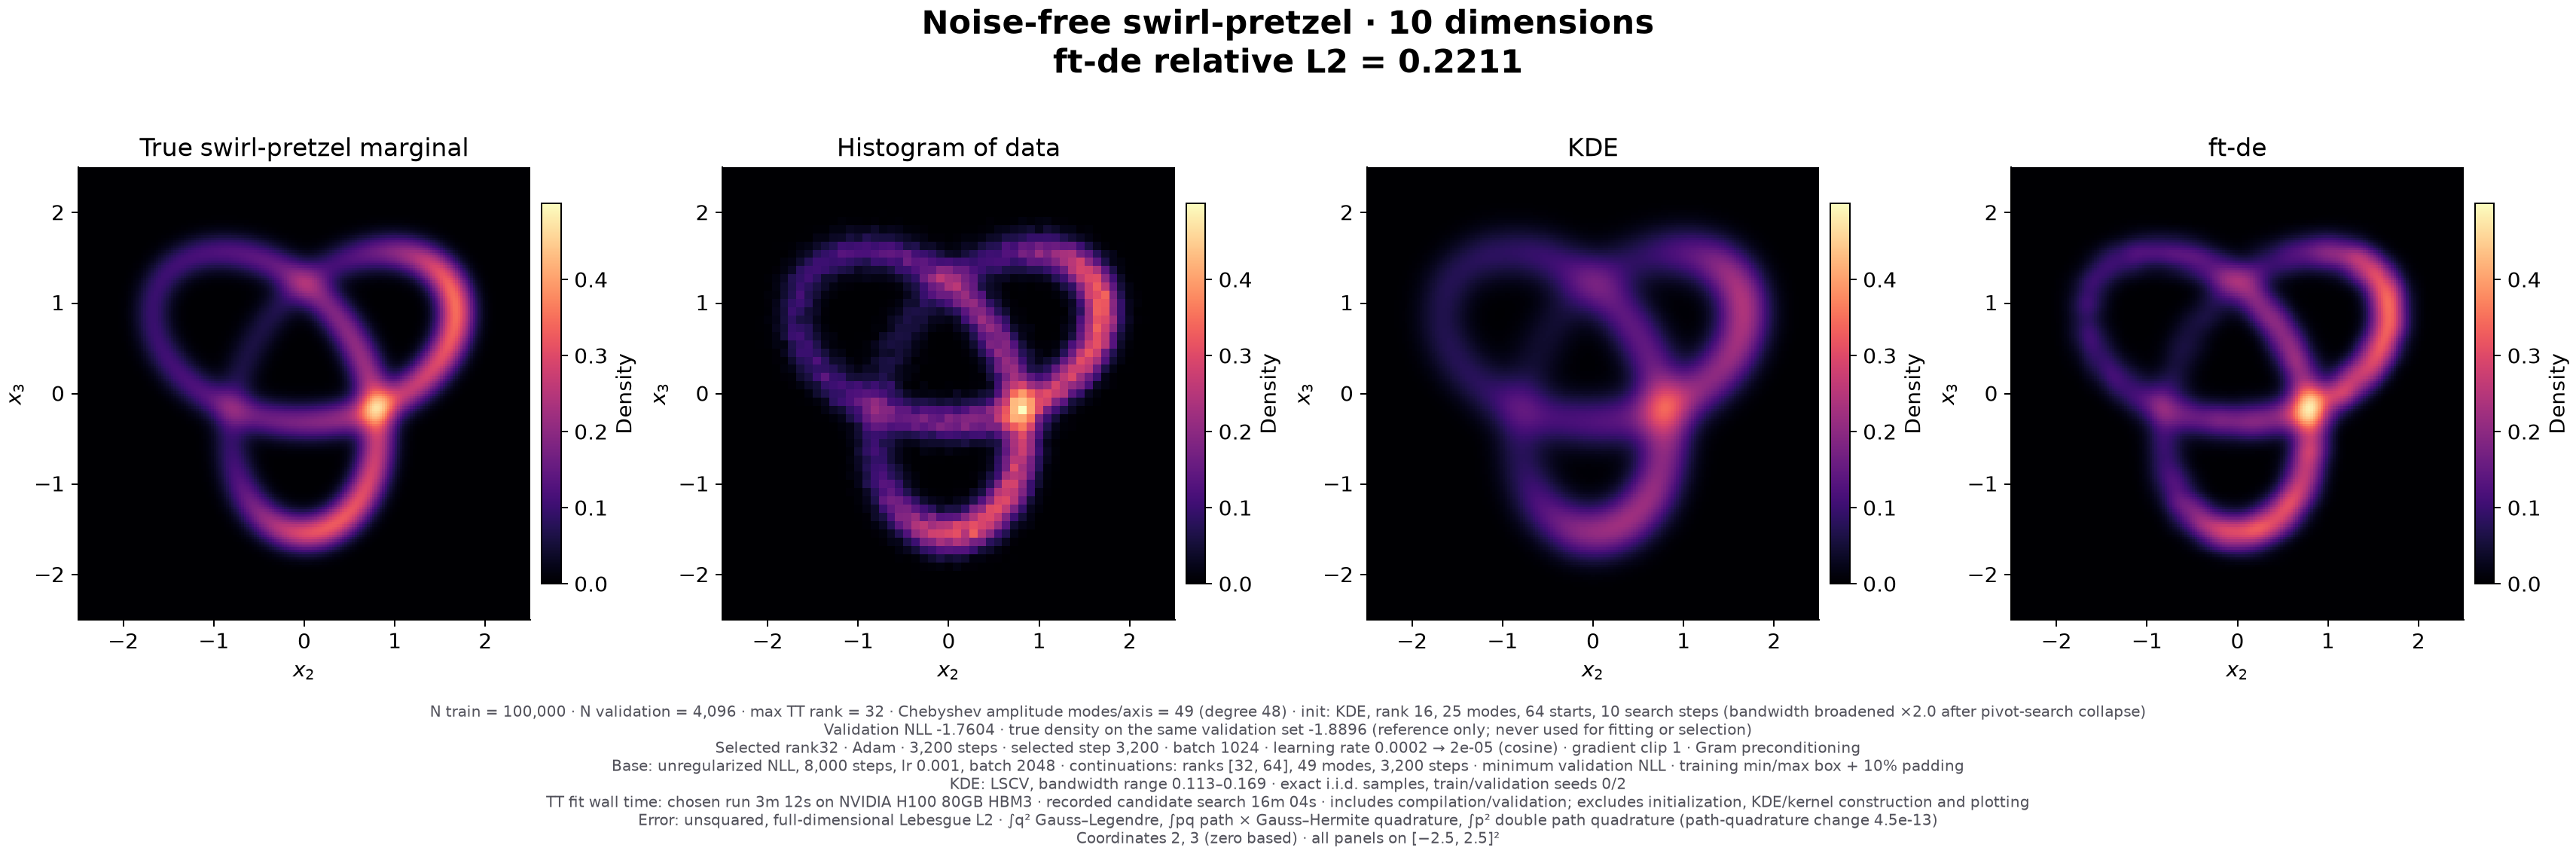
\includegraphics[width=\textwidth]{figures/sw_free_d10_23.png}\\[1mm]
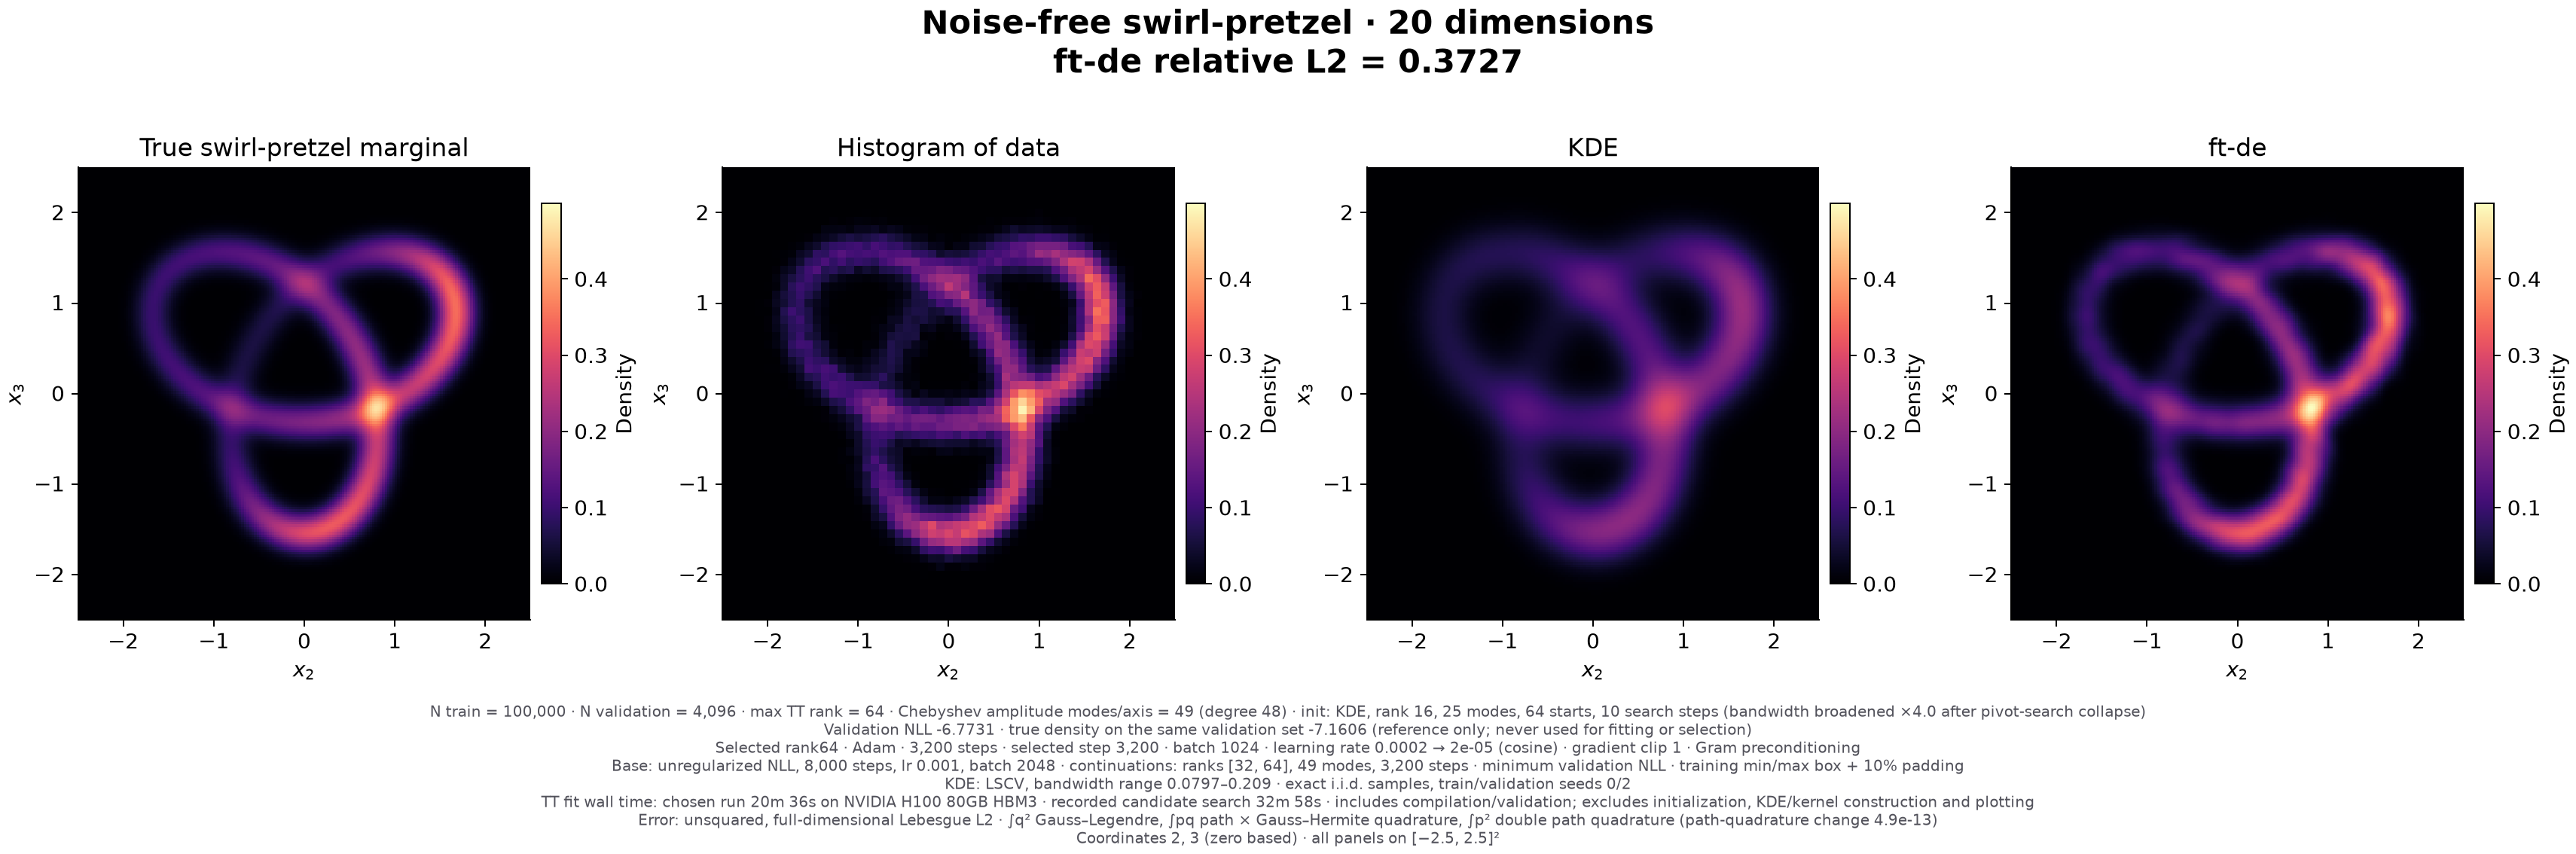
\includegraphics[width=\textwidth]{figures/sw_free_d20_23.png}
\caption{Noise-free swirl--pretzel, pretzel coordinates, $d=10$ (top) and $d=20$ (bottom). The recovered ridge is
continuous, with no beads, and sharper than the KDE.}
\label{fig:swirl-free}
\end{figure}

\begin{figure}[p]
\centering
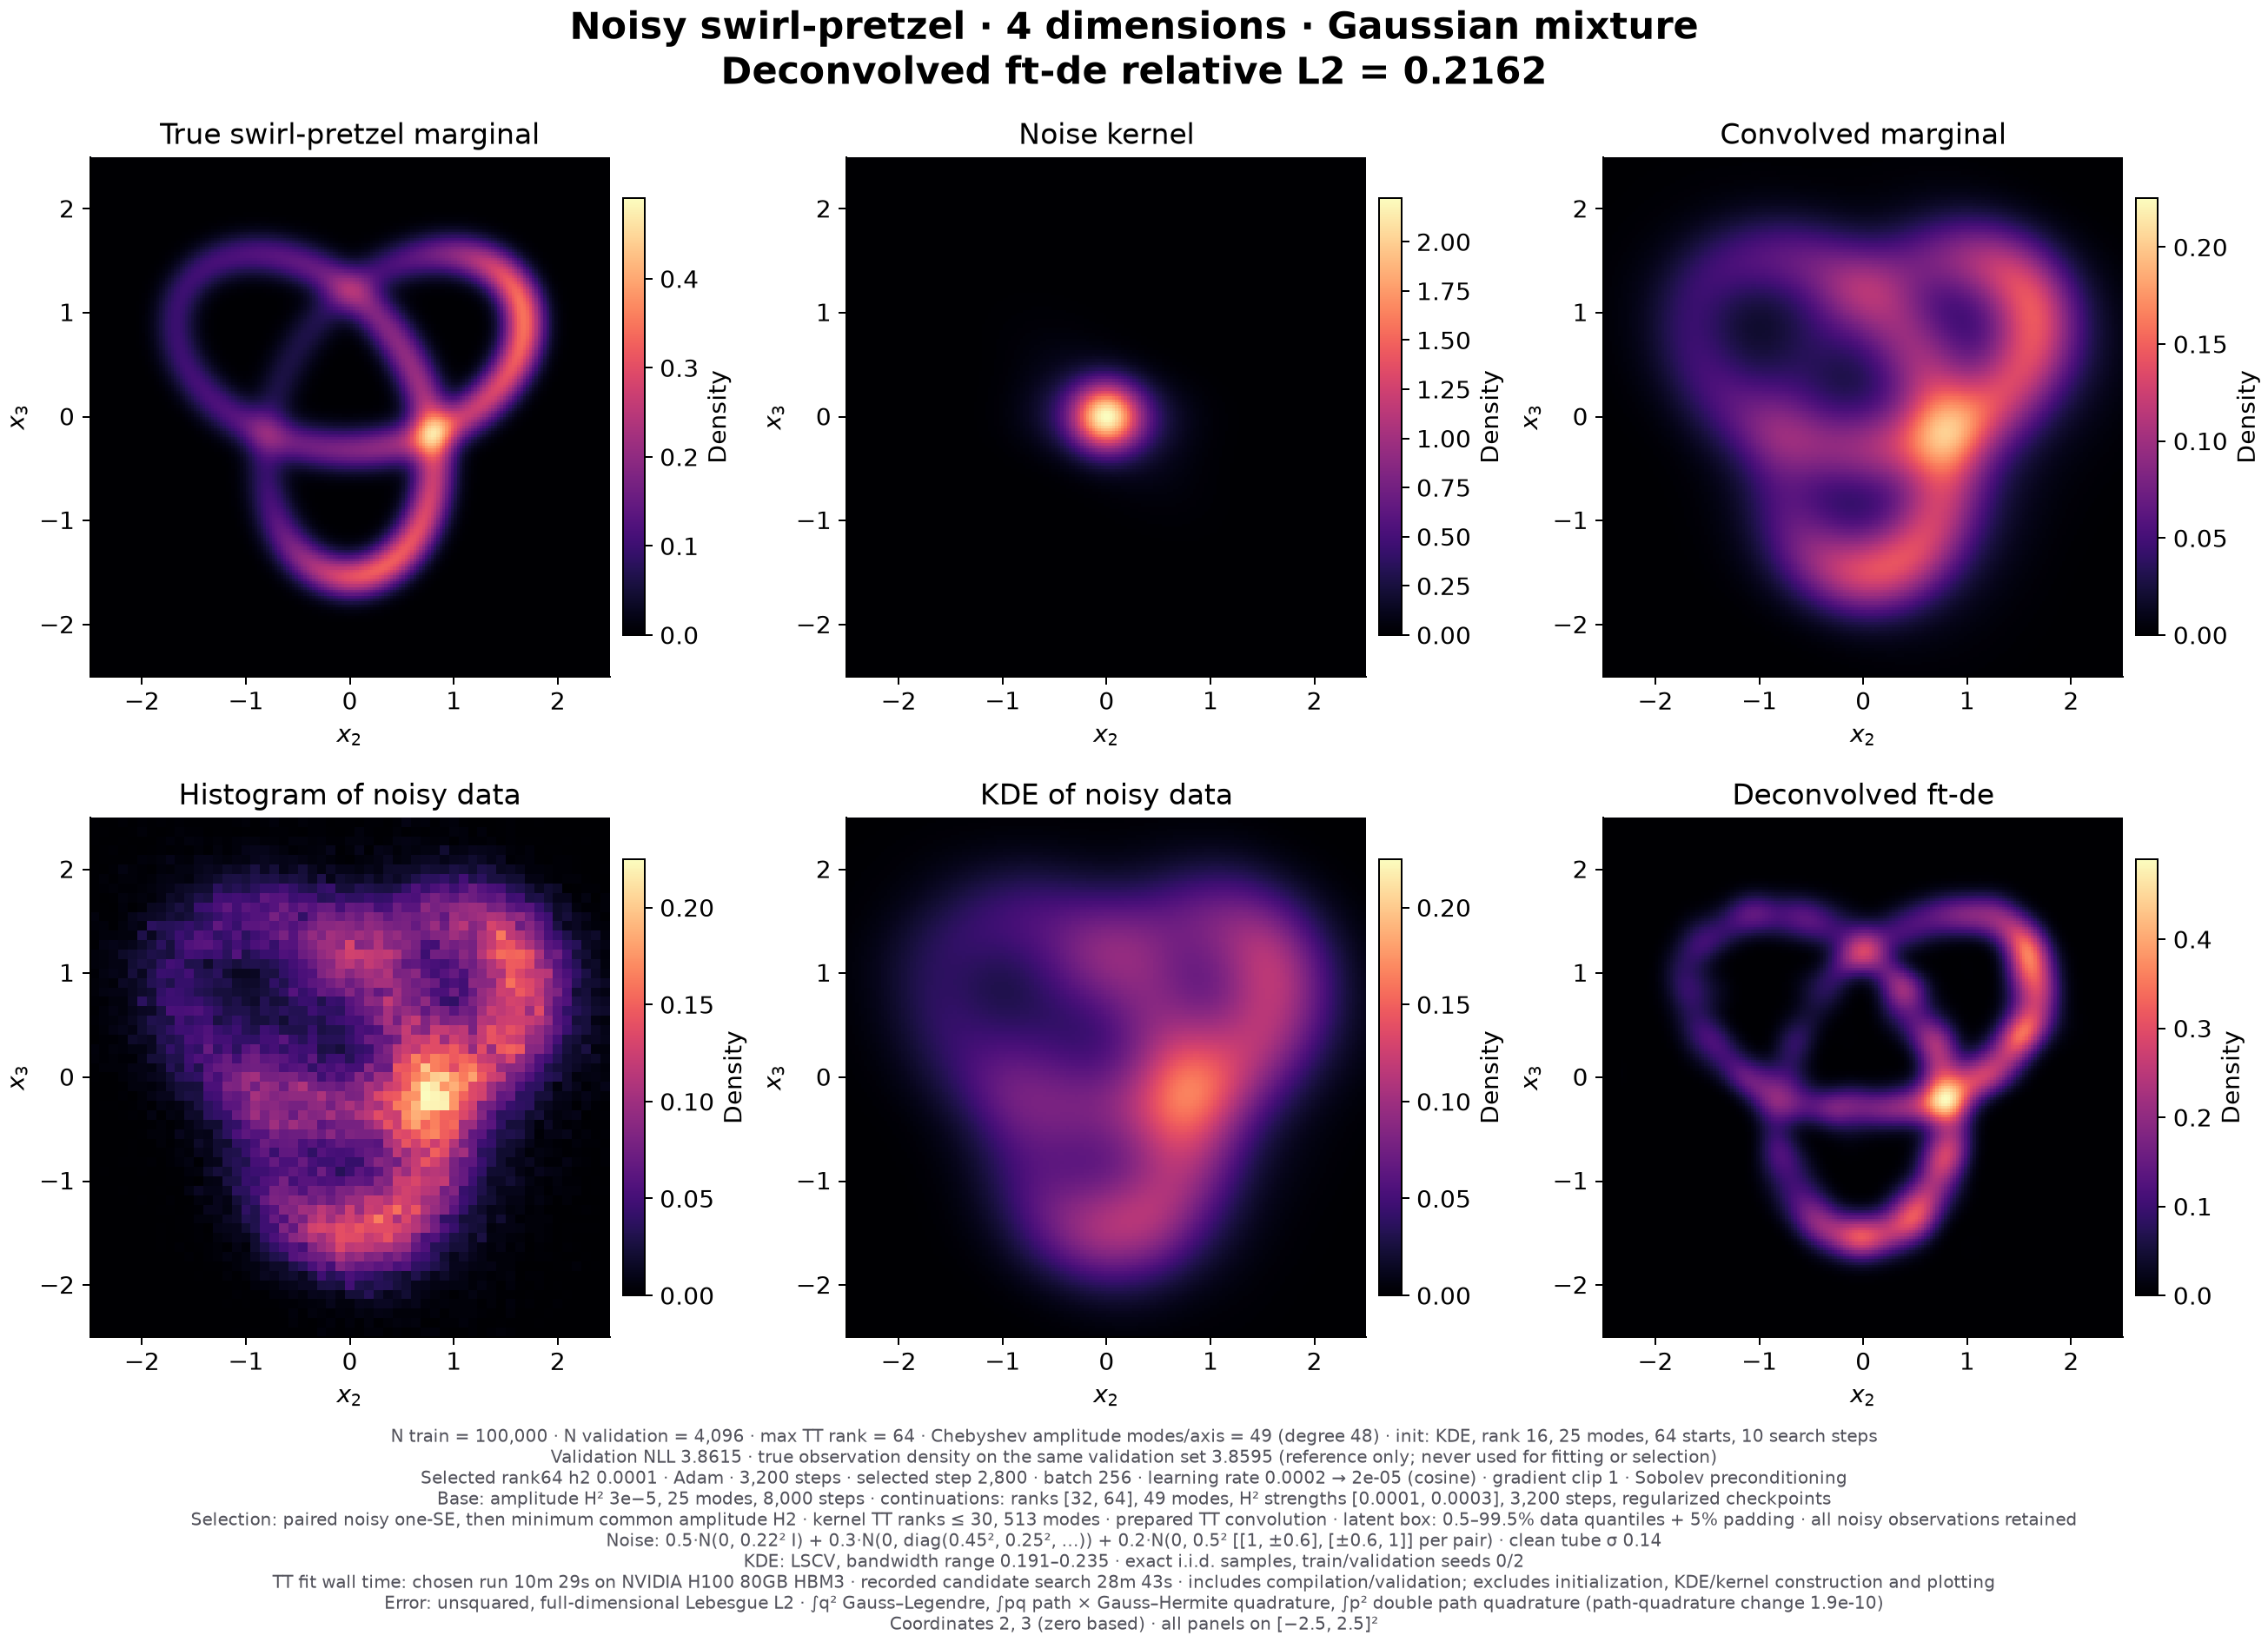
\includegraphics[width=.49\textwidth]{figures/sw_noisy_d4_23.png}\hfill
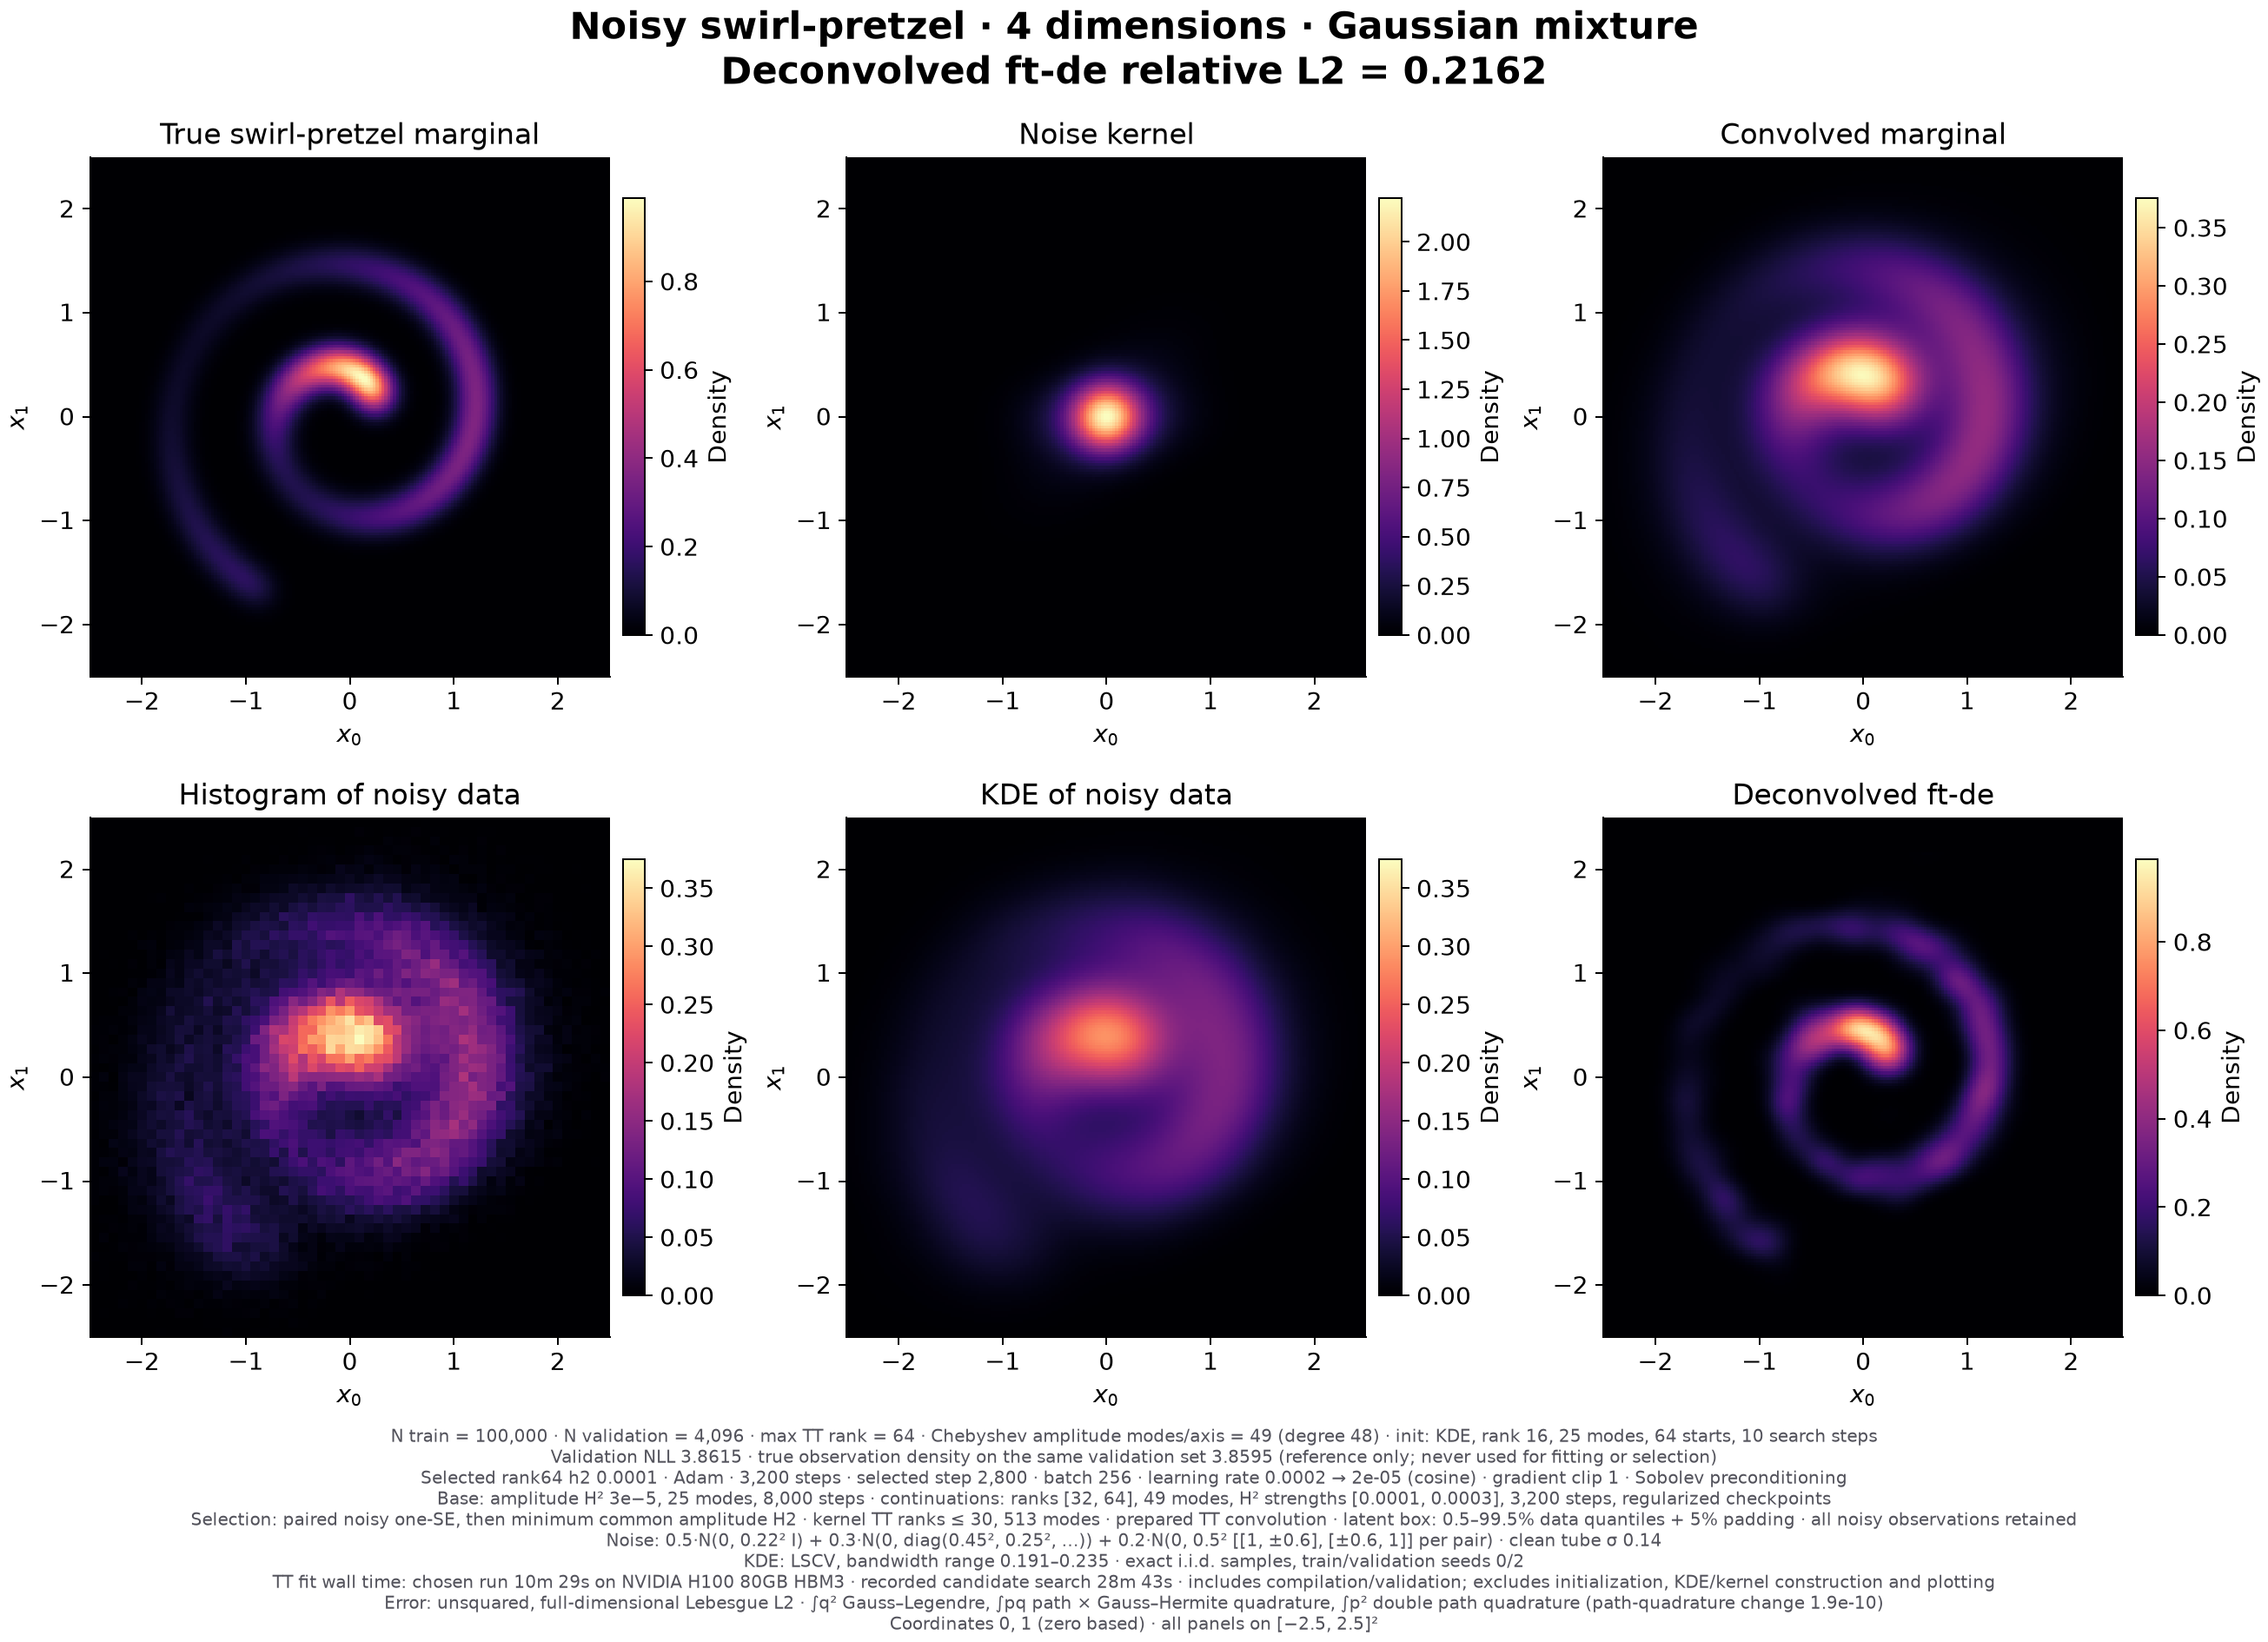
\includegraphics[width=.49\textwidth]{figures/sw_noisy_d4_01.png}\\[2mm]
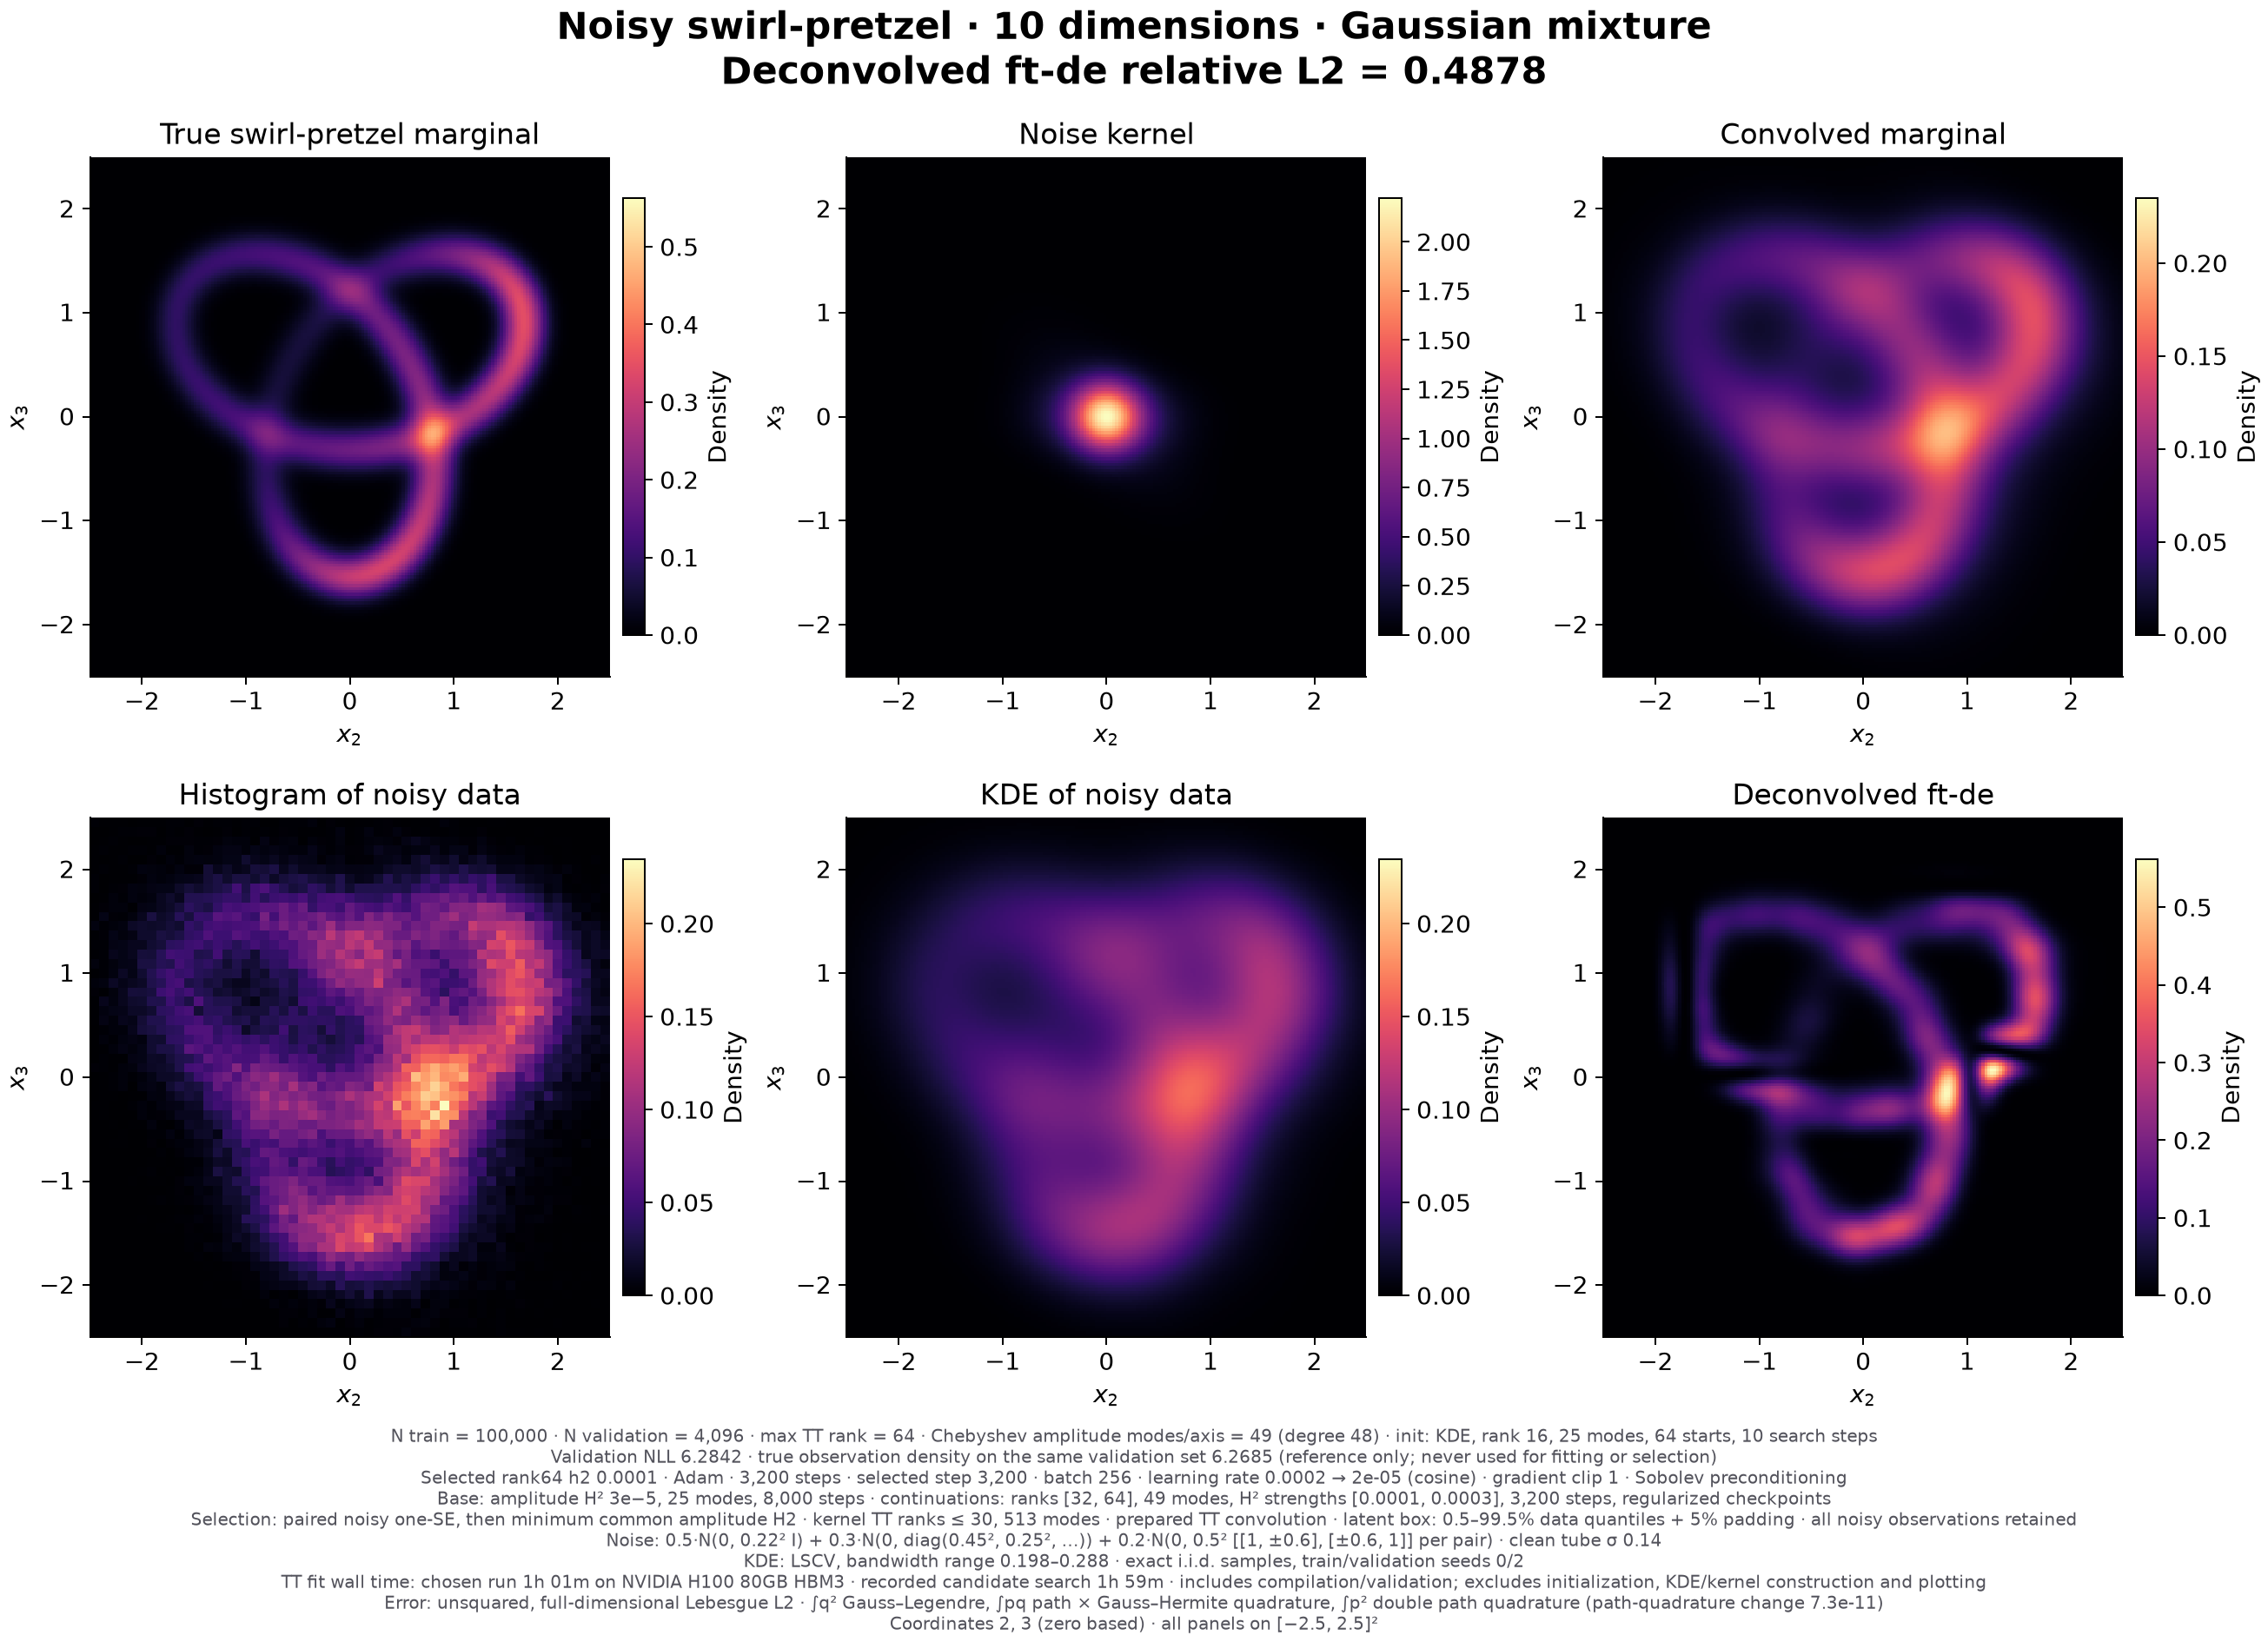
\includegraphics[width=.49\textwidth]{figures/sw_noisy_d10_23.png}\hfill
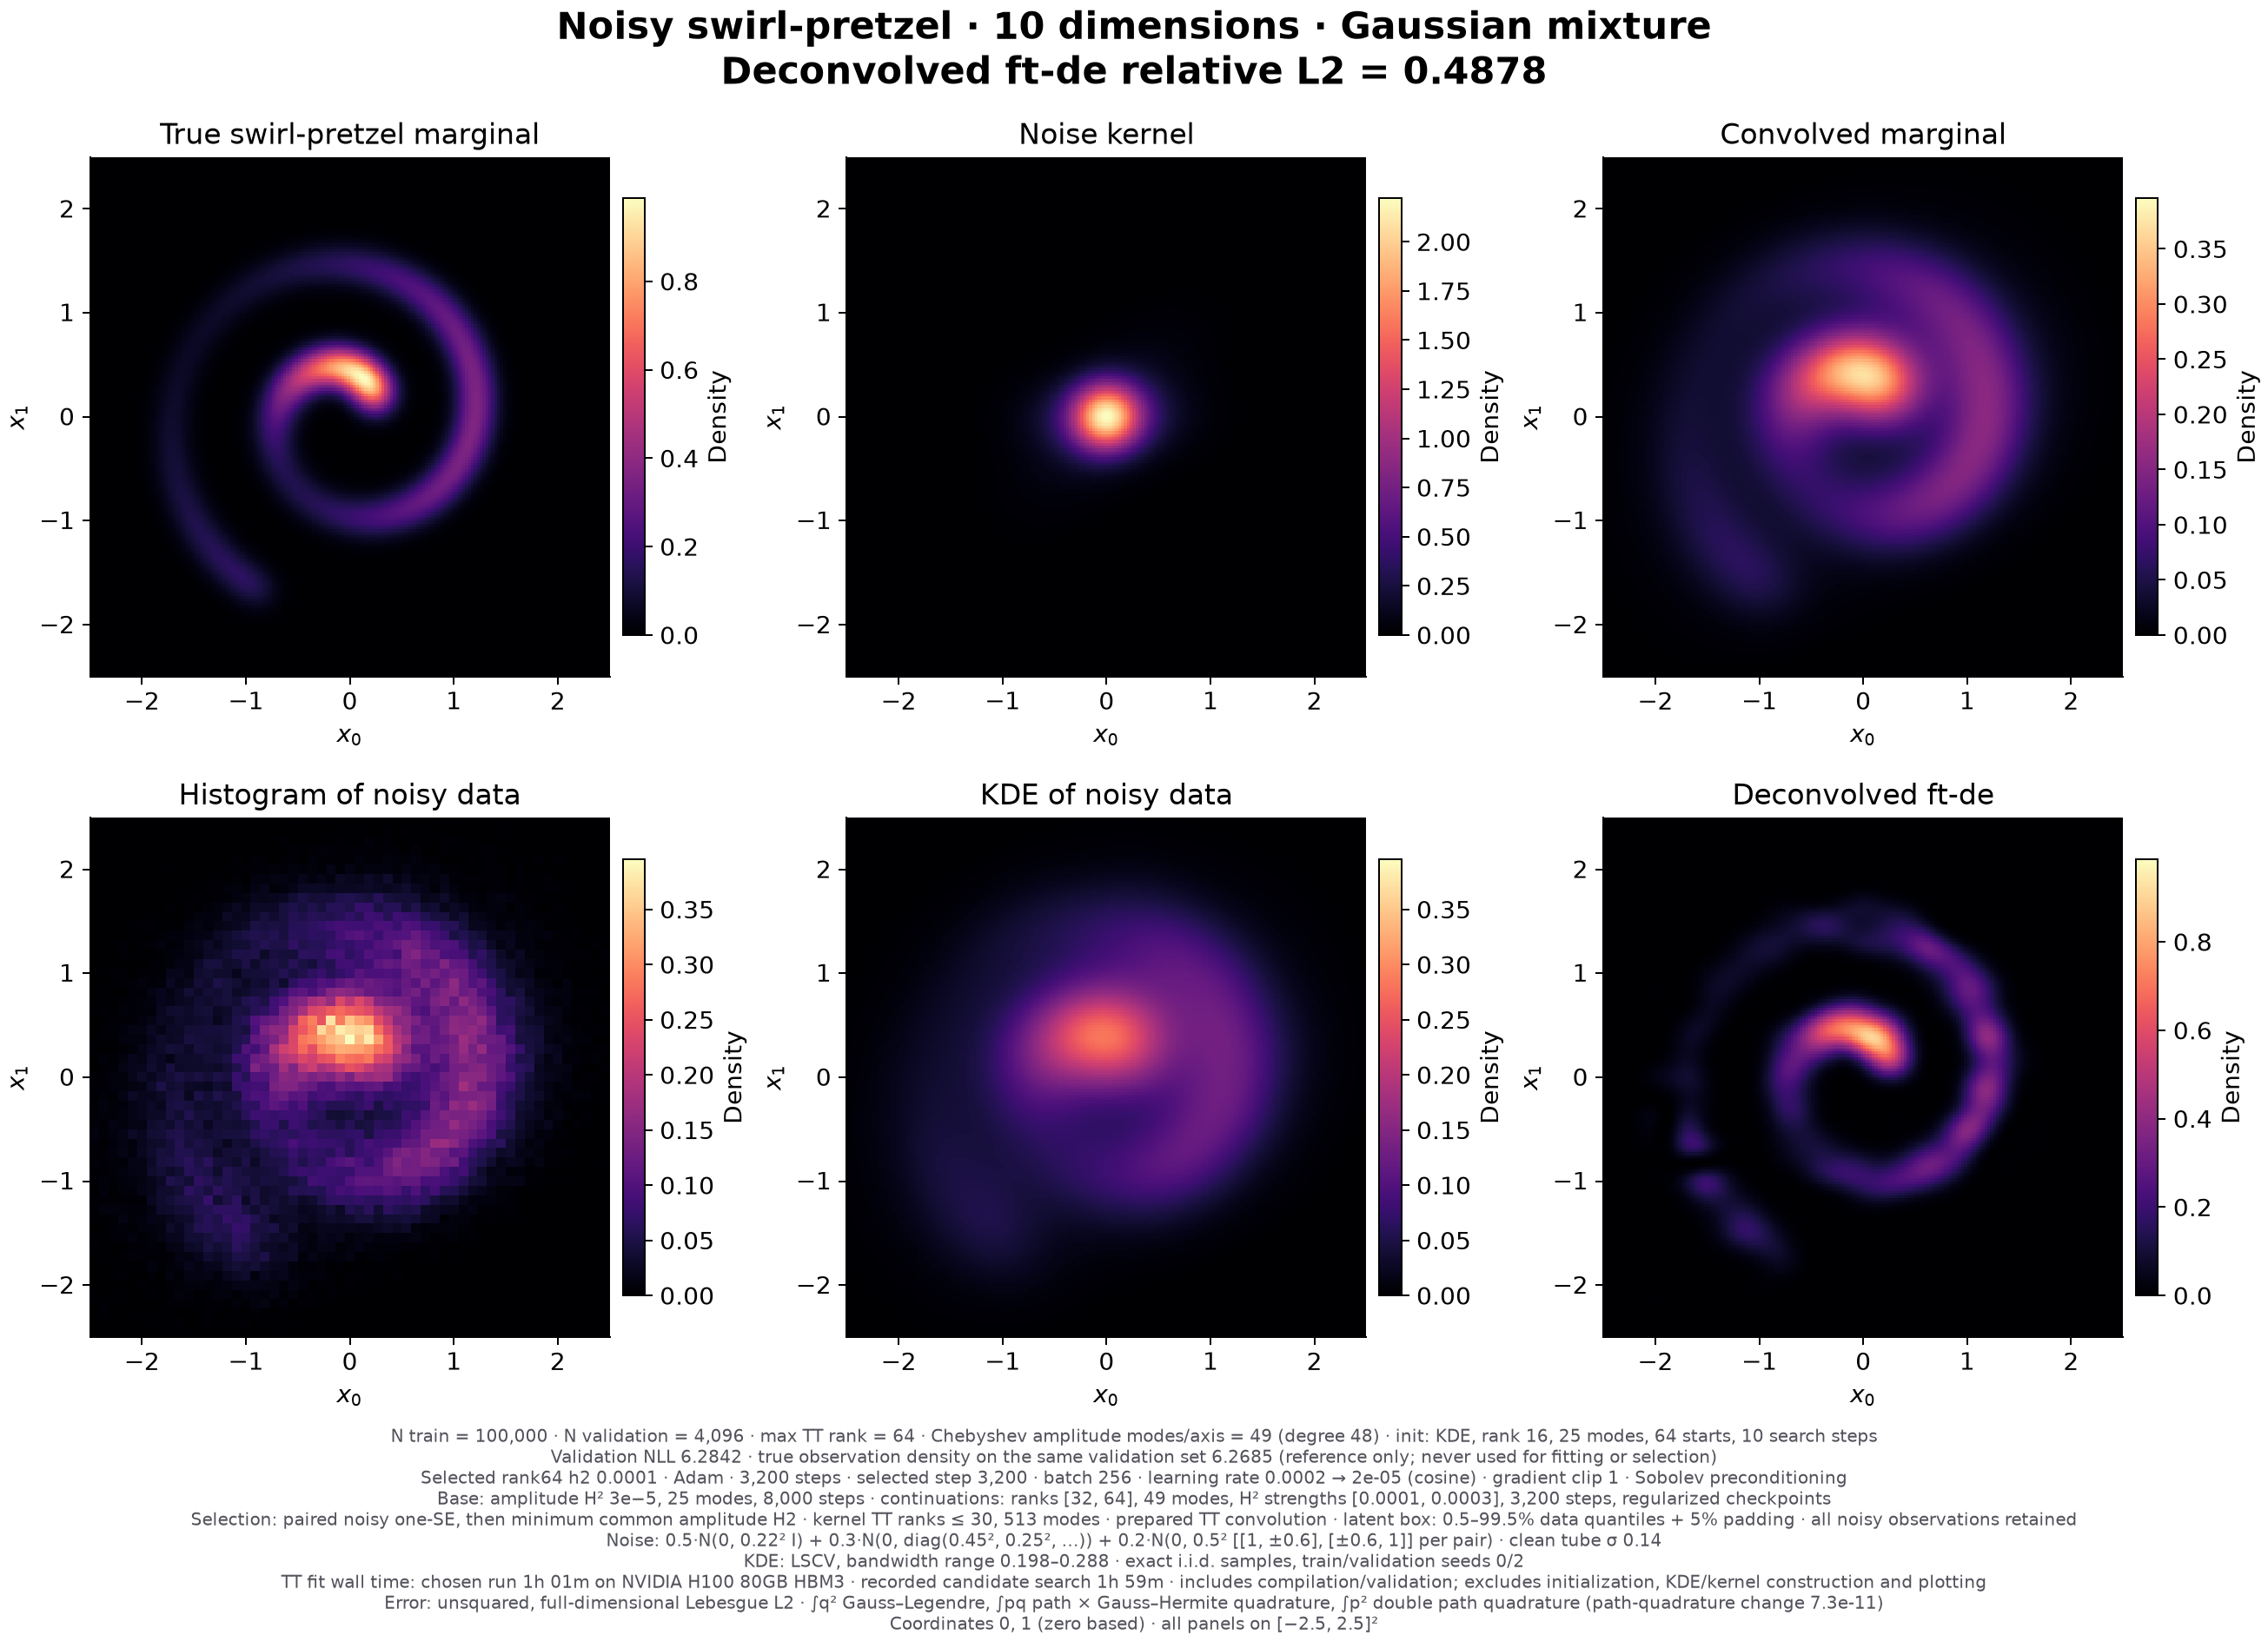
\includegraphics[width=.49\textwidth]{figures/sw_noisy_d10_01.png}
\caption{Noisy swirl--pretzel. Top: $d=4$; the deconvolved density (bottom right of each panel) recovers the
trefoil and the spiral, including the inner lobes that are invisible in the noisy histogram and KDE, with only faint
ripples. Bottom: $d=10$. The spiral's faint outer arm breaks into beads, and the pretzel has straight
axis-aligned segments, a spurious detached blob near $(1.3,0.1)$ and a missing crossing.}
\label{fig:swirl-noisy}
\end{figure}

\paragraph{Findings.}
\begin{enumerate}[leftmargin=2em,itemsep=2pt]
\item \emph{No noise, no beads.} In all dimensions the noise-free fits are continuous (Figure~\ref{fig:swirl-free}), with
ripple at most $3.7\%$ for every searched candidate. Representation and optimization alone do not fragment
ridges. Rank-64, 49-mode fits show faint ripple along the ridge from the global Chebyshev basis, far below bead
contrast.
\item \emph{Deconvolution in $d=4$ is nearly as good as the data allow.} The selected fit is within
$0.0021\pm0.0010$ nats of the true noisy density, and its marginals are continuous
(Figure~\ref{fig:swirl-noisy}, top).
\item \emph{Deconvolution in $d=10$ fragments ridges} (Figure~\ref{fig:swirl-noisy}, bottom; ripple on the pretzel
$16$--$19\%$). The artifacts are already present in the rank-16 base fit, and every continuation inherits them
(Figure~\ref{fig:cand10}). The noisy likelihood \emph{does} detect that this fit is wrong: the truth scores
$0.0157\pm0.0027$ nats better, about six standard errors. The failure is therefore not an identifiability limit
at this $N$. The optimizer is stuck in a worse basin. Figure~\ref{fig:seeds} repeats the $d=10$ fit (rank 32, $\lambda=3\cdot10^{-4}$) from three chebdGE initializations
(different KDE subsamples and pivot searches). All three reach the same noisy NLL within noise (gaps to the truth
$0.030$, $0.033$, $0.031$, each $\pm0.004$) and the same latent error ($\relLtwo=0.588,0.588,0.600$). The artifacts, however,
sit in \emph{different places}: a detached blob, vertical and horizontal streaks, or a broken spiral arm. The
normalized-density average of the three has the same noisy NLL as its best member ($\Delta=0.0003\pm0.0007$), yet
its pretzel marginal is markedly closer to the truth (2D relative $L^2$ $0.18$ against $0.21$--$0.26$). Artifact
\emph{locations} are therefore basin-dependent and invisible to the noisy likelihood. Agreement across independent
initializations is a diagnostic the likelihood cannot provide.
\item \emph{In $d=20$} the pretzel marginal is again mostly continuous, with a broken upper-left lobe
(Figure~\ref{fig:swirl20}), but the fit is far from the truth in full dimension ($\relLtwo=0.87$; NLL gap
$0.160\pm0.008$ nats). With a fixed budget of steps and rank, the gap to the truth grows with $d$ both with and without
noise (Table~\ref{tab:swirl}).
\item \emph{Held-out noisy NLL tracks latent error} (Figure~\ref{fig:gap}). Across every searched candidate, in every
dimension, a smaller gap to the true observation density goes with a smaller latent $\relLtwo$. The only inversion,
between the two rank-32 fits in $d=10$, is within one standard error. The
one-standard-error rule therefore selects sensibly among the candidates it is offered. Its weakness is that it only
chooses among fits that share the base fit's topology.
\item \emph{Smoothing trades beads for bias} (Figure~\ref{fig:h2}). Raising the amplitude-$H^2$ strength in $d=10$
from $10^{-4}$ to $10^{-2}$ removes the spiral beads (ripple $0.050\to0.008$) and halves the pretzel ripple
($0.19\to0.10$). But $\relLtwo$ rises from $0.55$ to $0.90$ and the NLL gap from $0.030$ to $0.109$ nats. The
pretzel's misplaced segments remain, only blurred. Beads are a visible but minor part of the error.
\end{enumerate}

\begin{figure}[t]
\centering
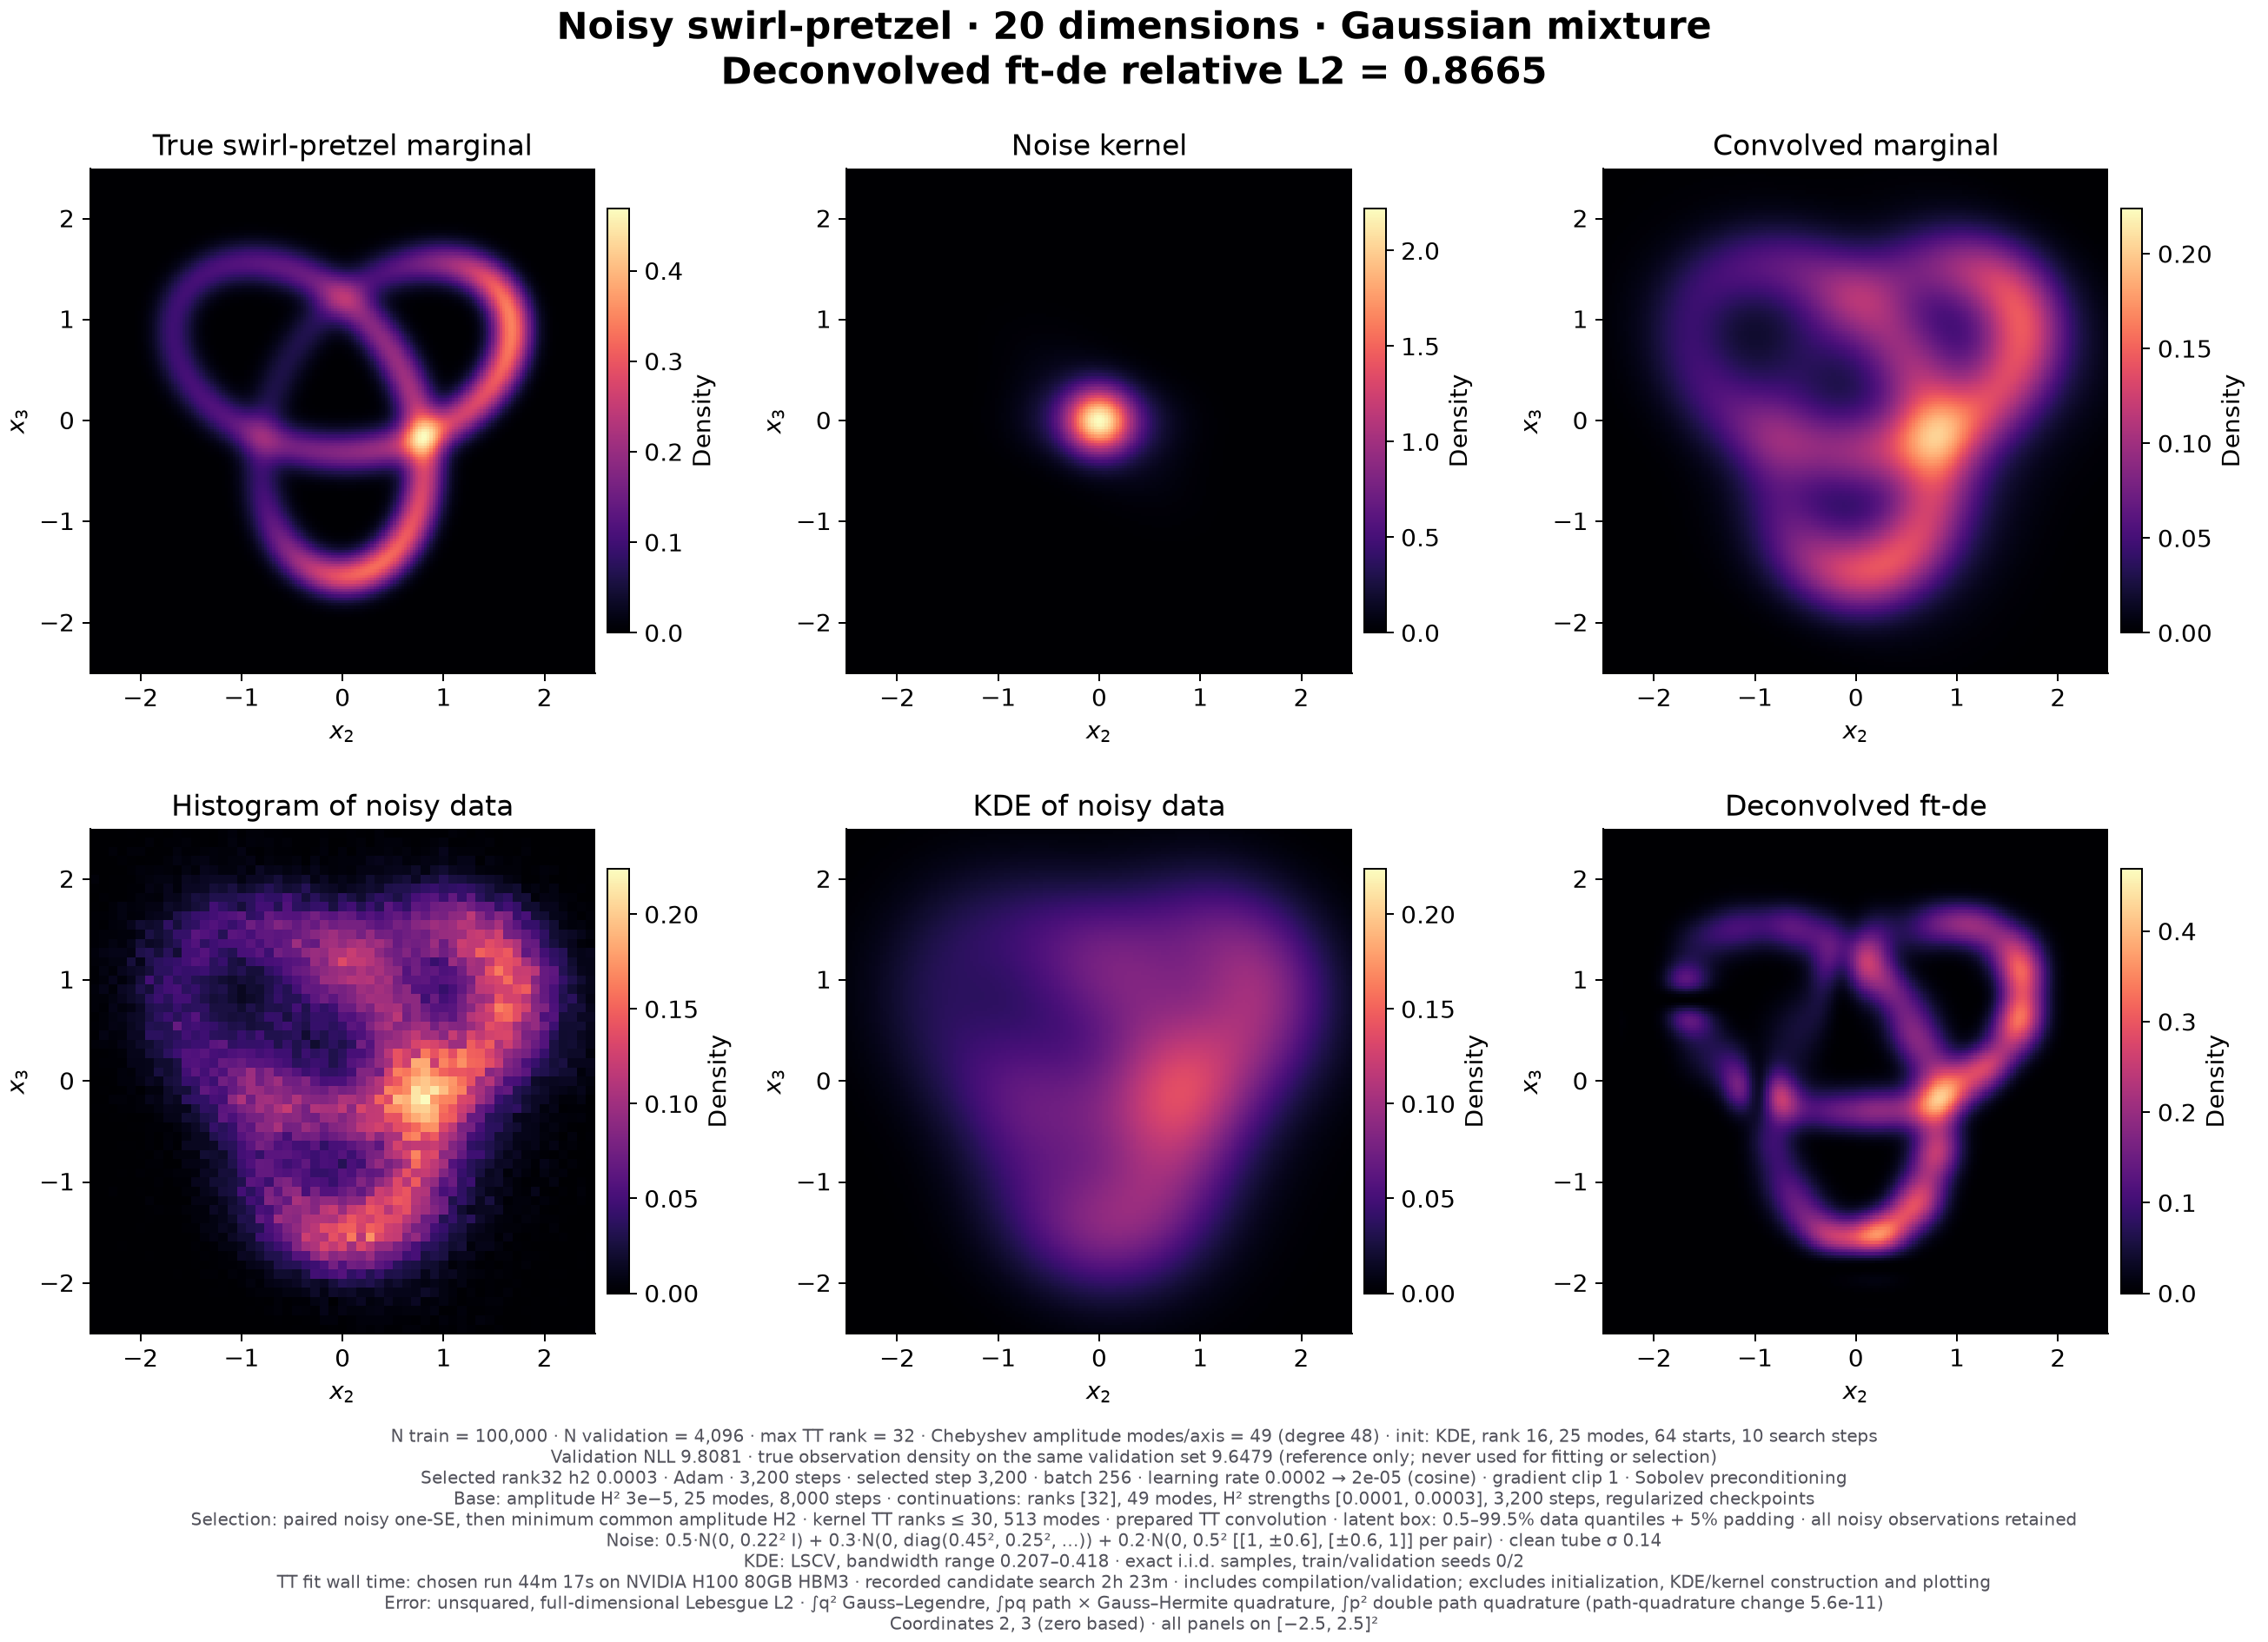
\includegraphics[width=.49\textwidth]{figures/sw_noisy_d20_23.png}\hfill
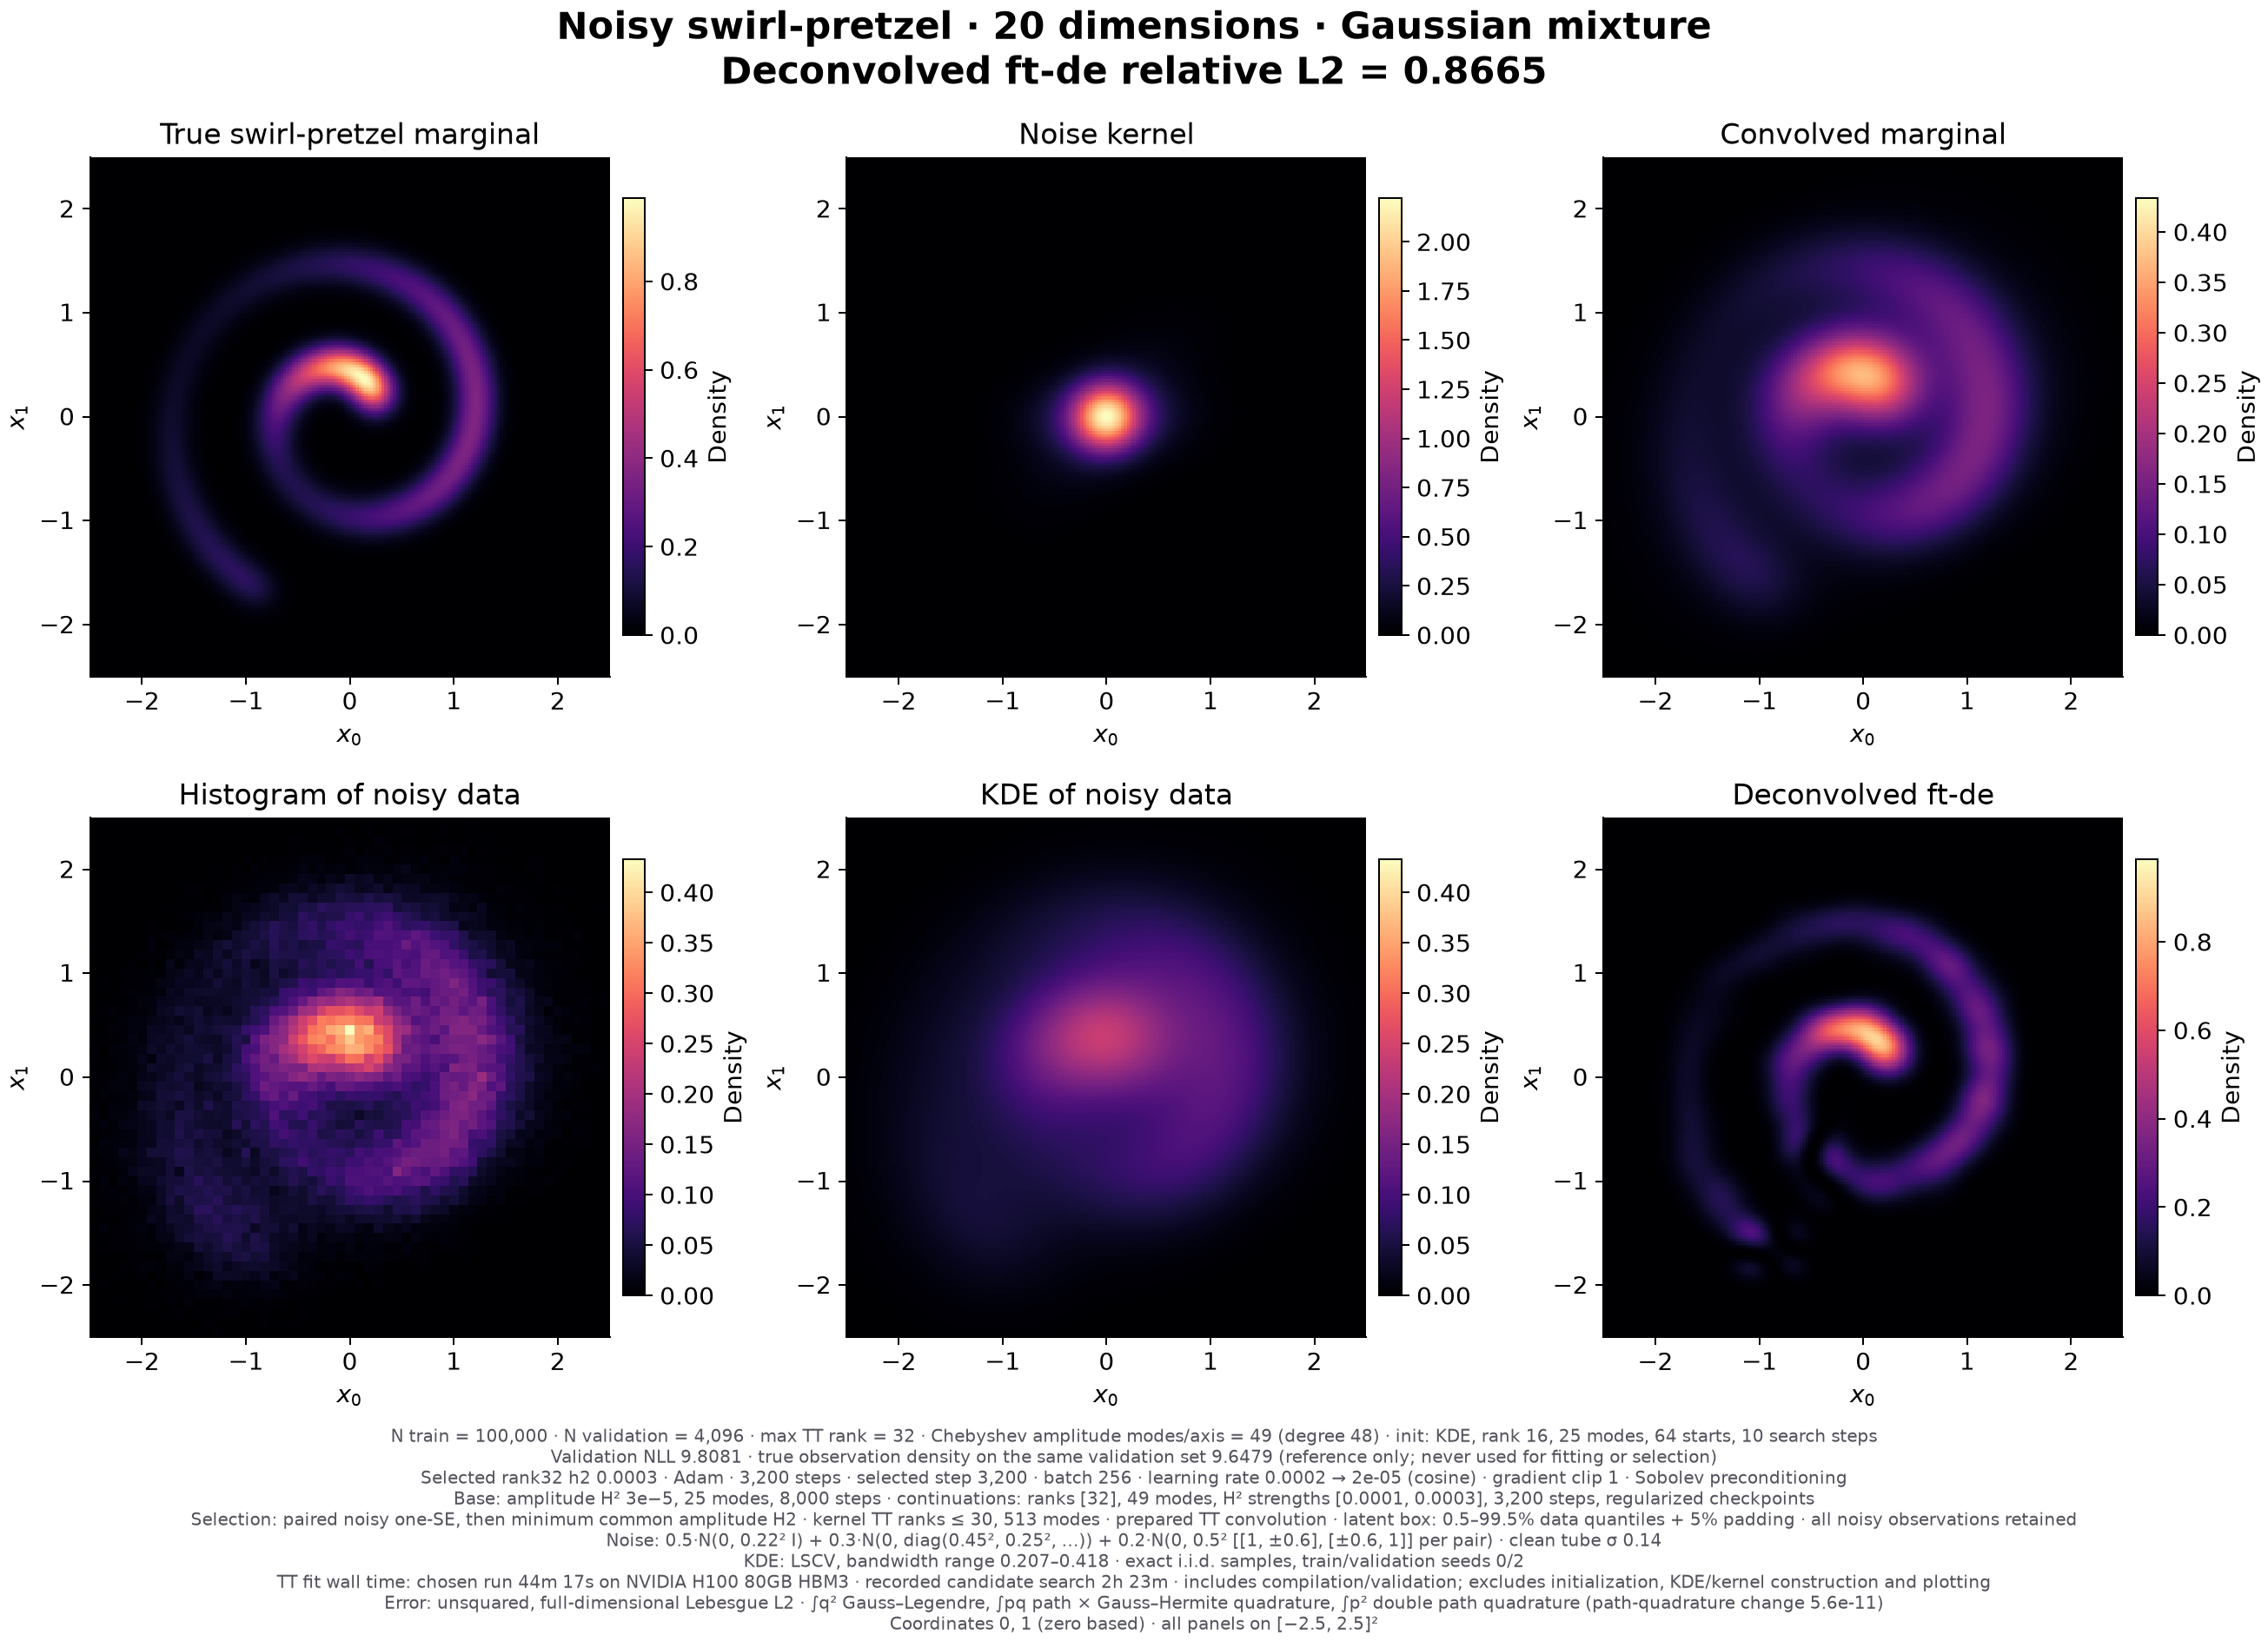
\includegraphics[width=.49\textwidth]{figures/sw_noisy_d20_01.png}
\caption{Noisy swirl--pretzel, $d=20$ (rank 32, $\lambda=3\cdot10^{-4}$).}
\label{fig:swirl20}
\end{figure}

\begin{figure}[p]
\centering
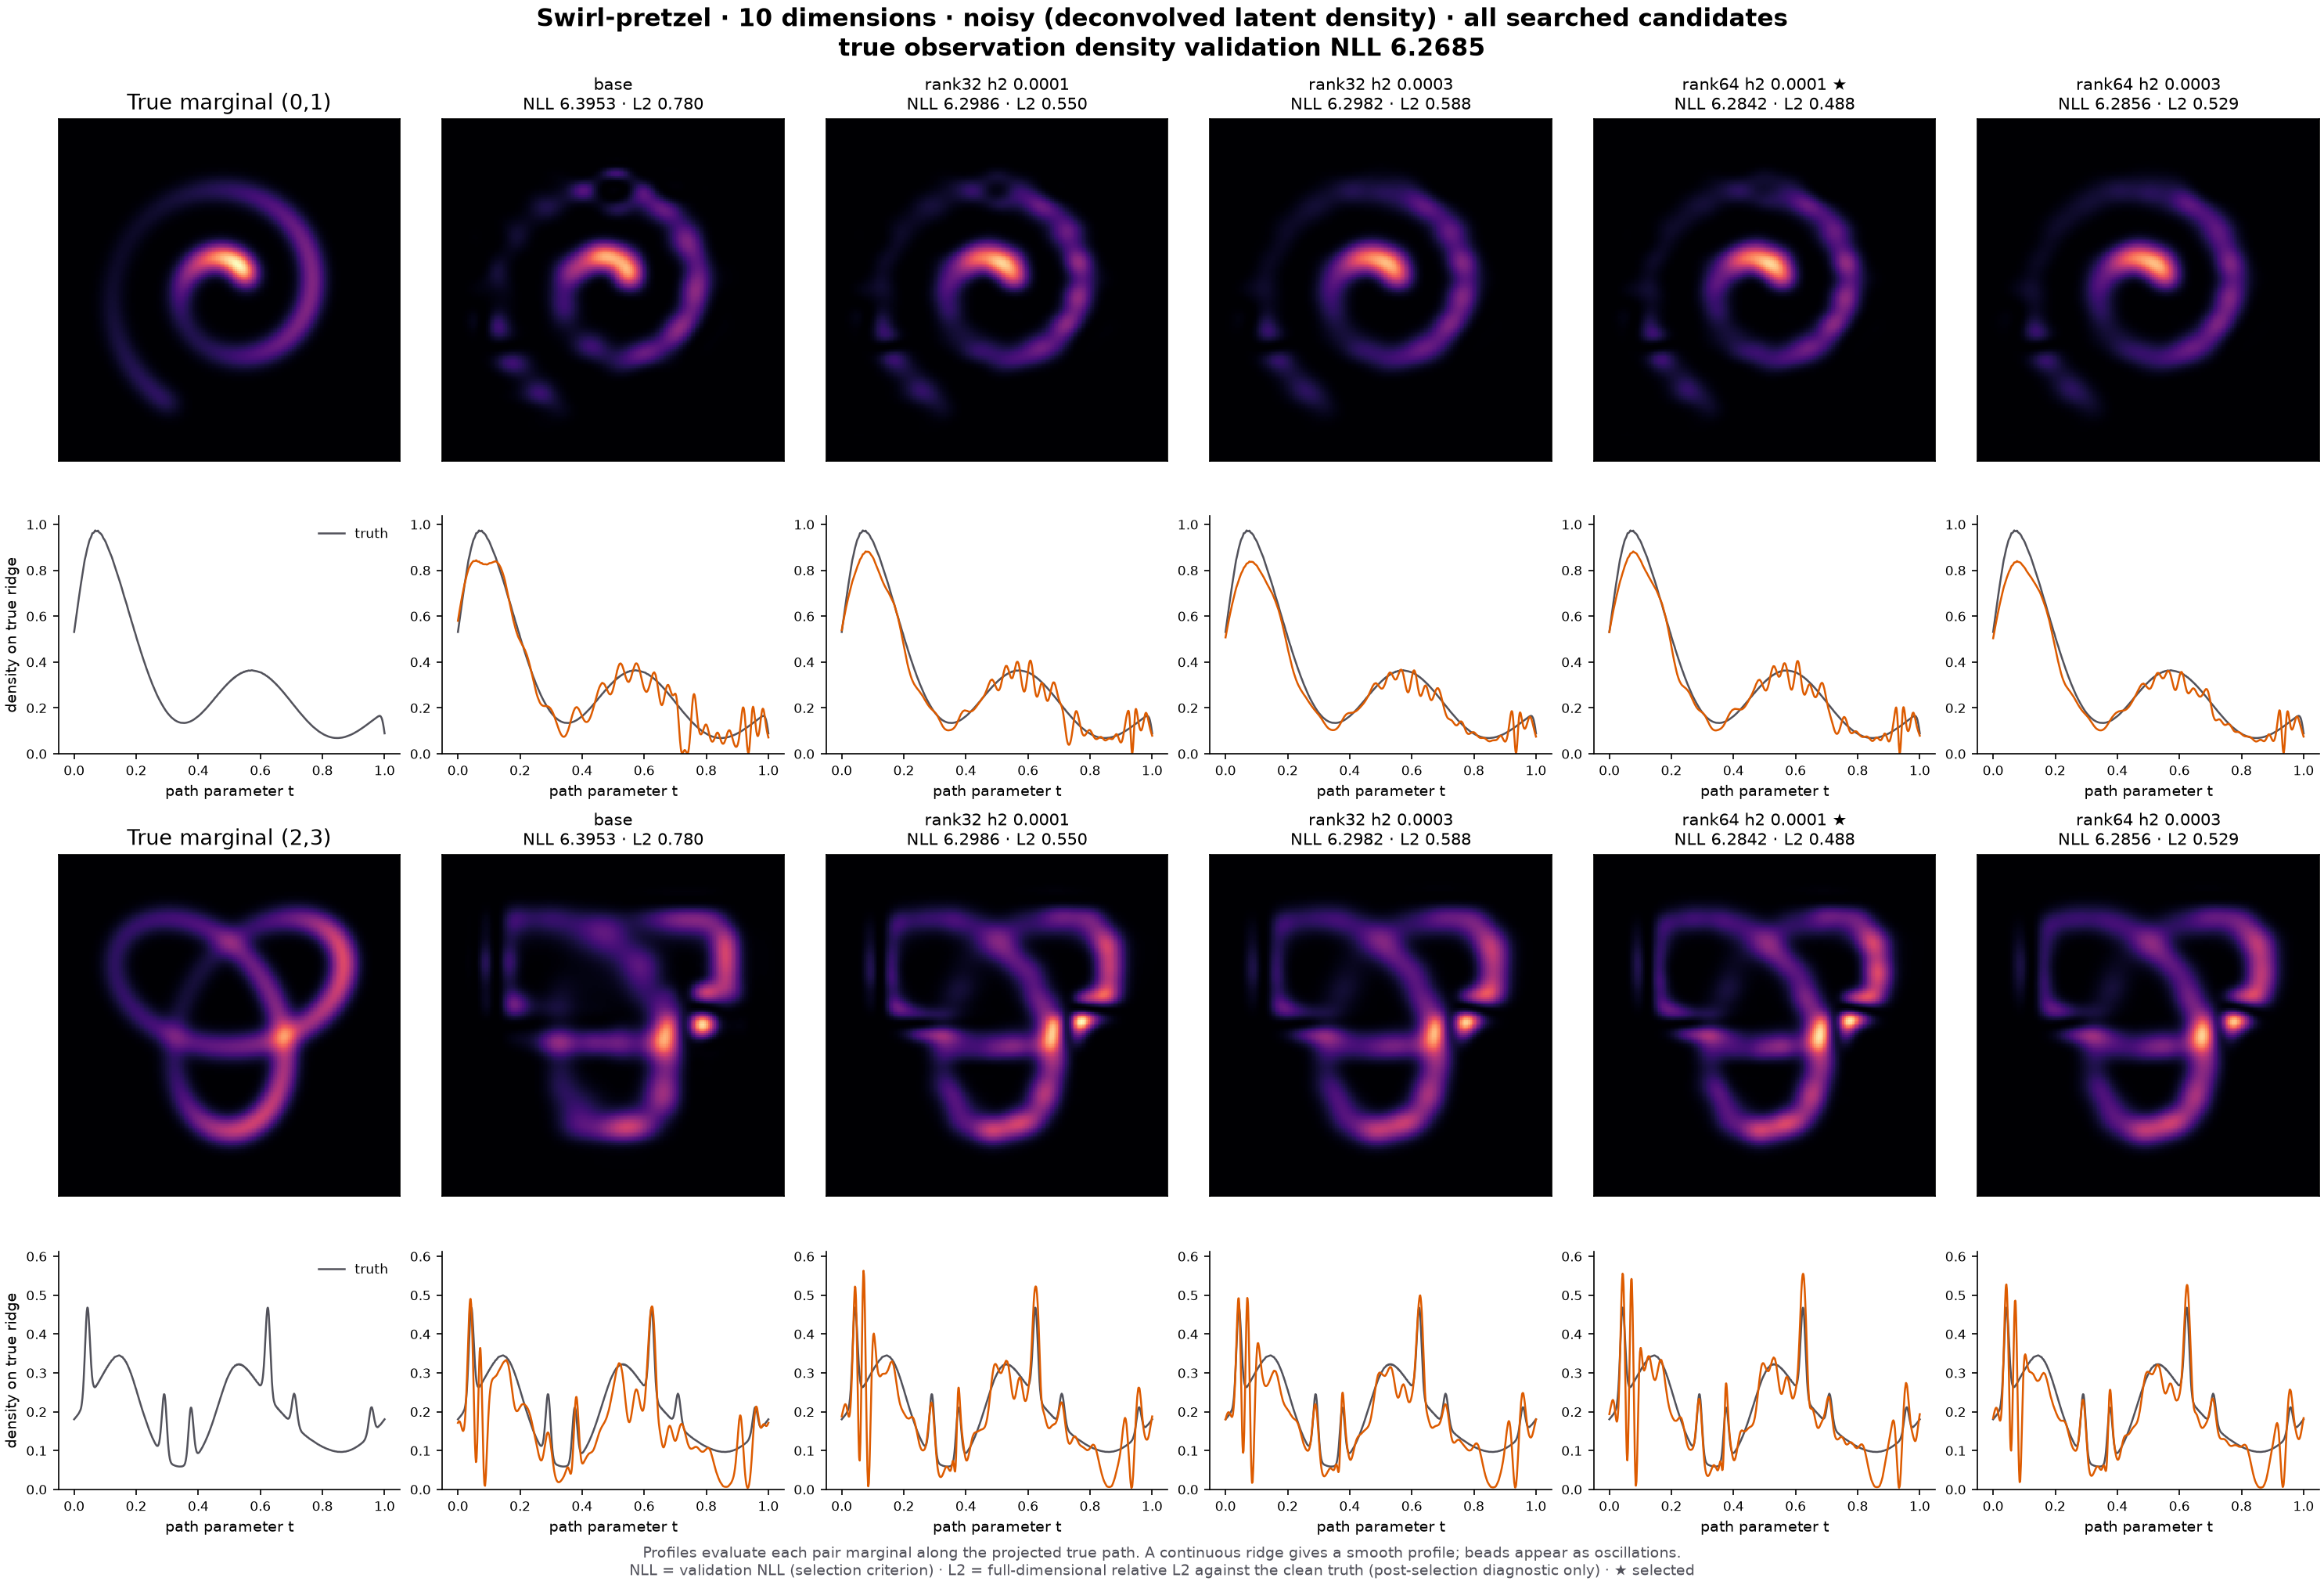
\includegraphics[width=\textwidth]{figures/sw_cand_noisy_d10.png}
\caption{Every searched candidate for the $d=10$ noisy swirl--pretzel (base, rank 32 and 64, $H^2$ strengths
$10^{-4}$ and $3\cdot10^{-4}$). The profiles underneath evaluate each pair marginal along the projected true path
(gray: truth; orange: estimate). The pretzel's spurious blob and straight segments are present in the base fit and
in every continuation.}
\label{fig:cand10}
\end{figure}

\begin{figure}[t]
\centering
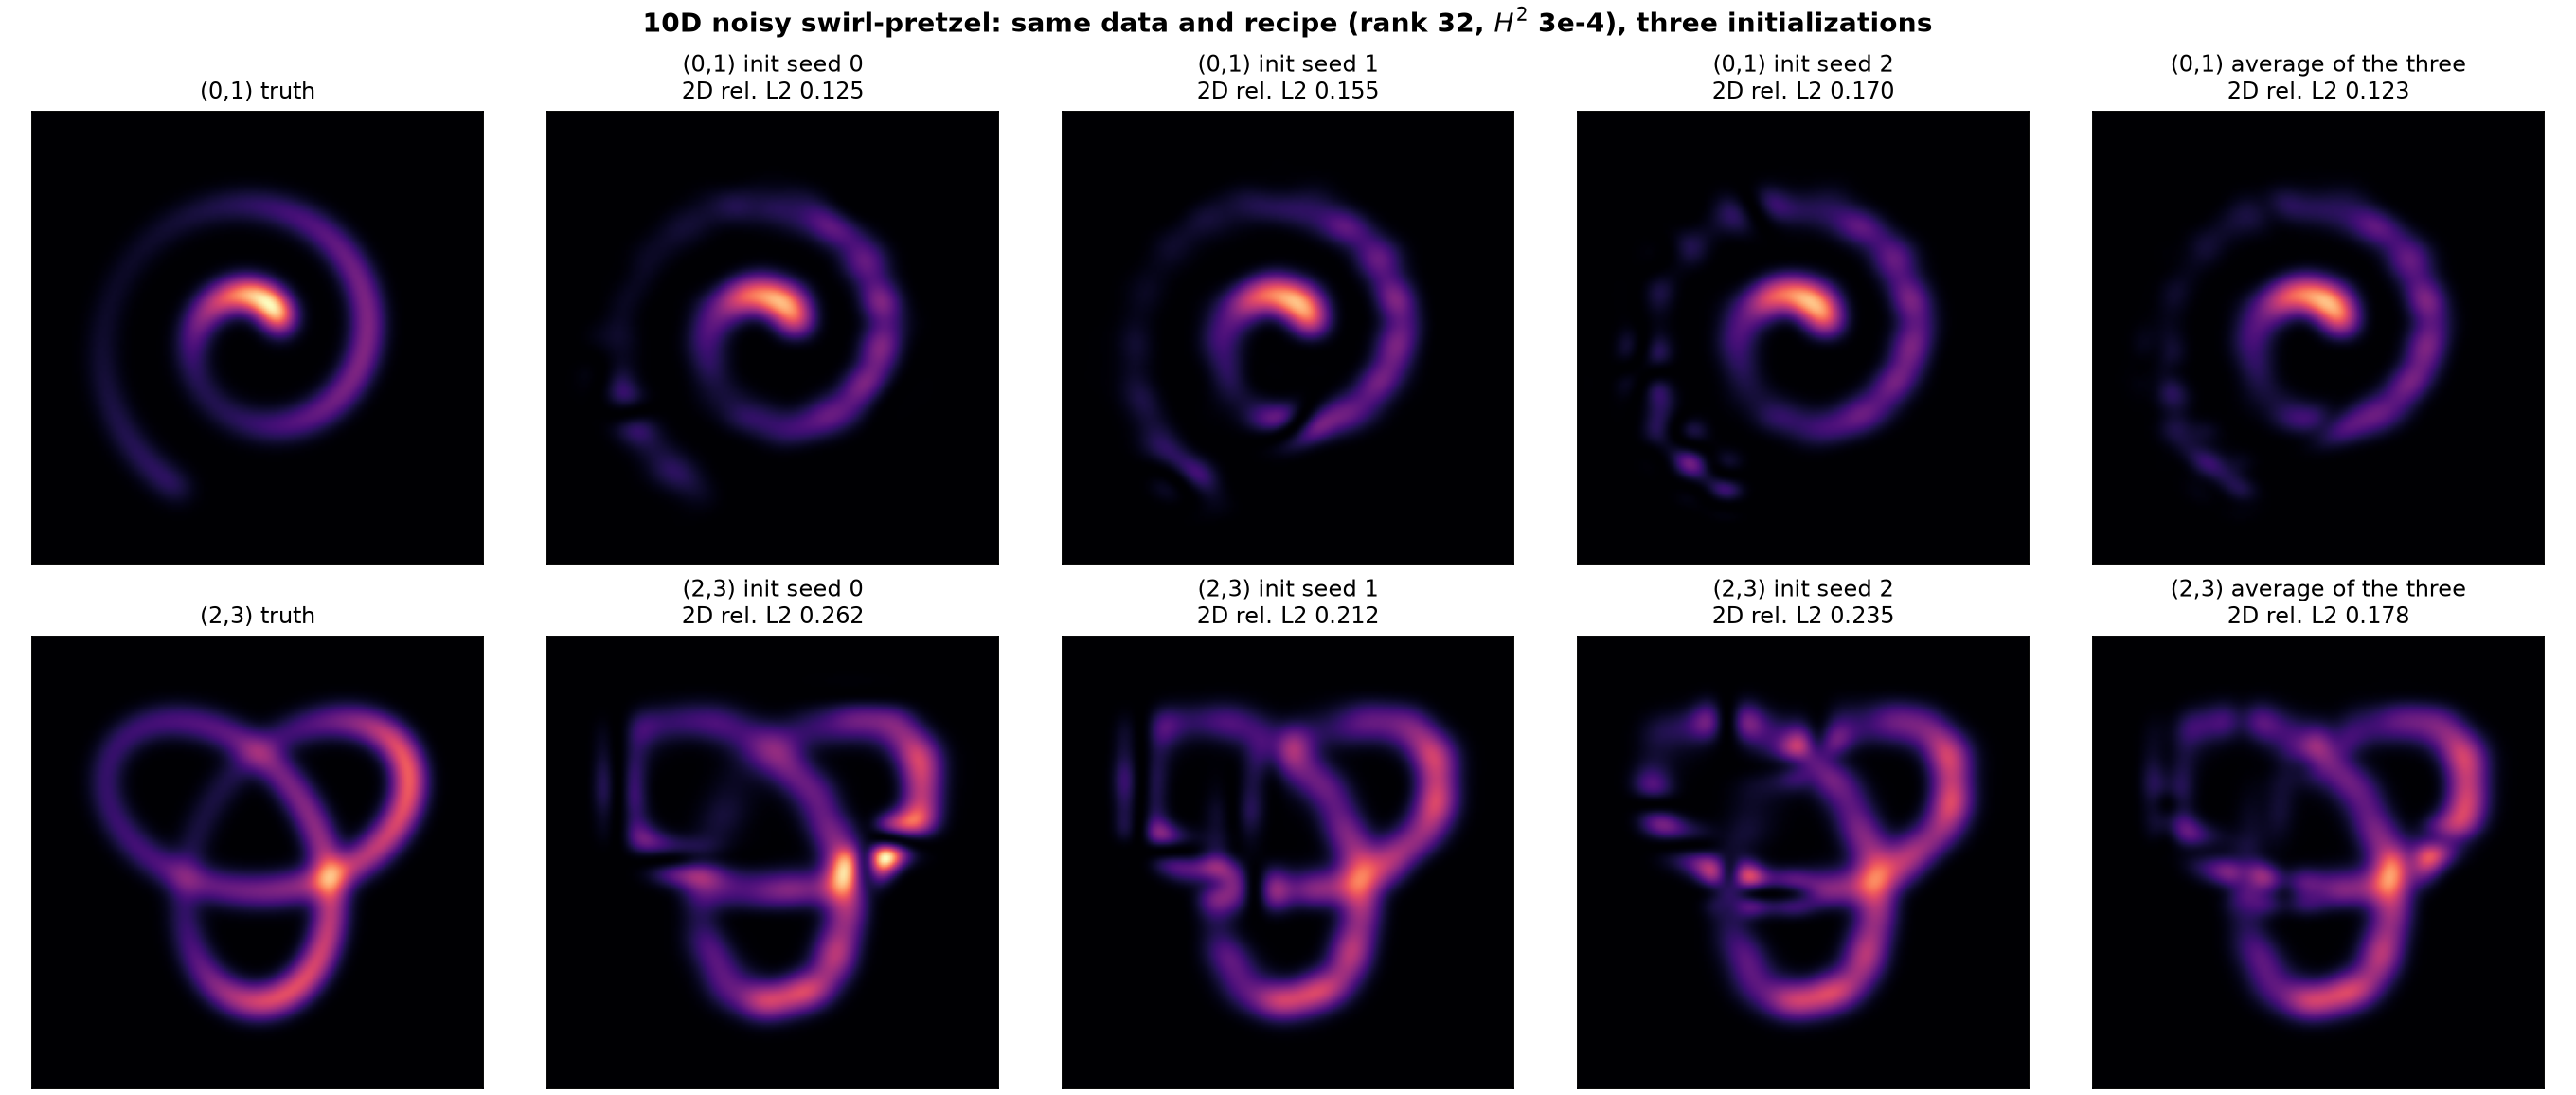
\includegraphics[width=\textwidth]{figures/init_seeds.png}
\caption{$d=10$ noisy swirl--pretzel: the same data and recipe from three chebdGE initializations, and the average of
their normalized densities. The noisy validation NLL cannot distinguish the four (gaps to the truth
$0.030$--$0.033\pm0.004$ nats), but the artifacts move between initializations and partly cancel in the average.}
\label{fig:seeds}
\end{figure}

\begin{figure}[t]
\centering
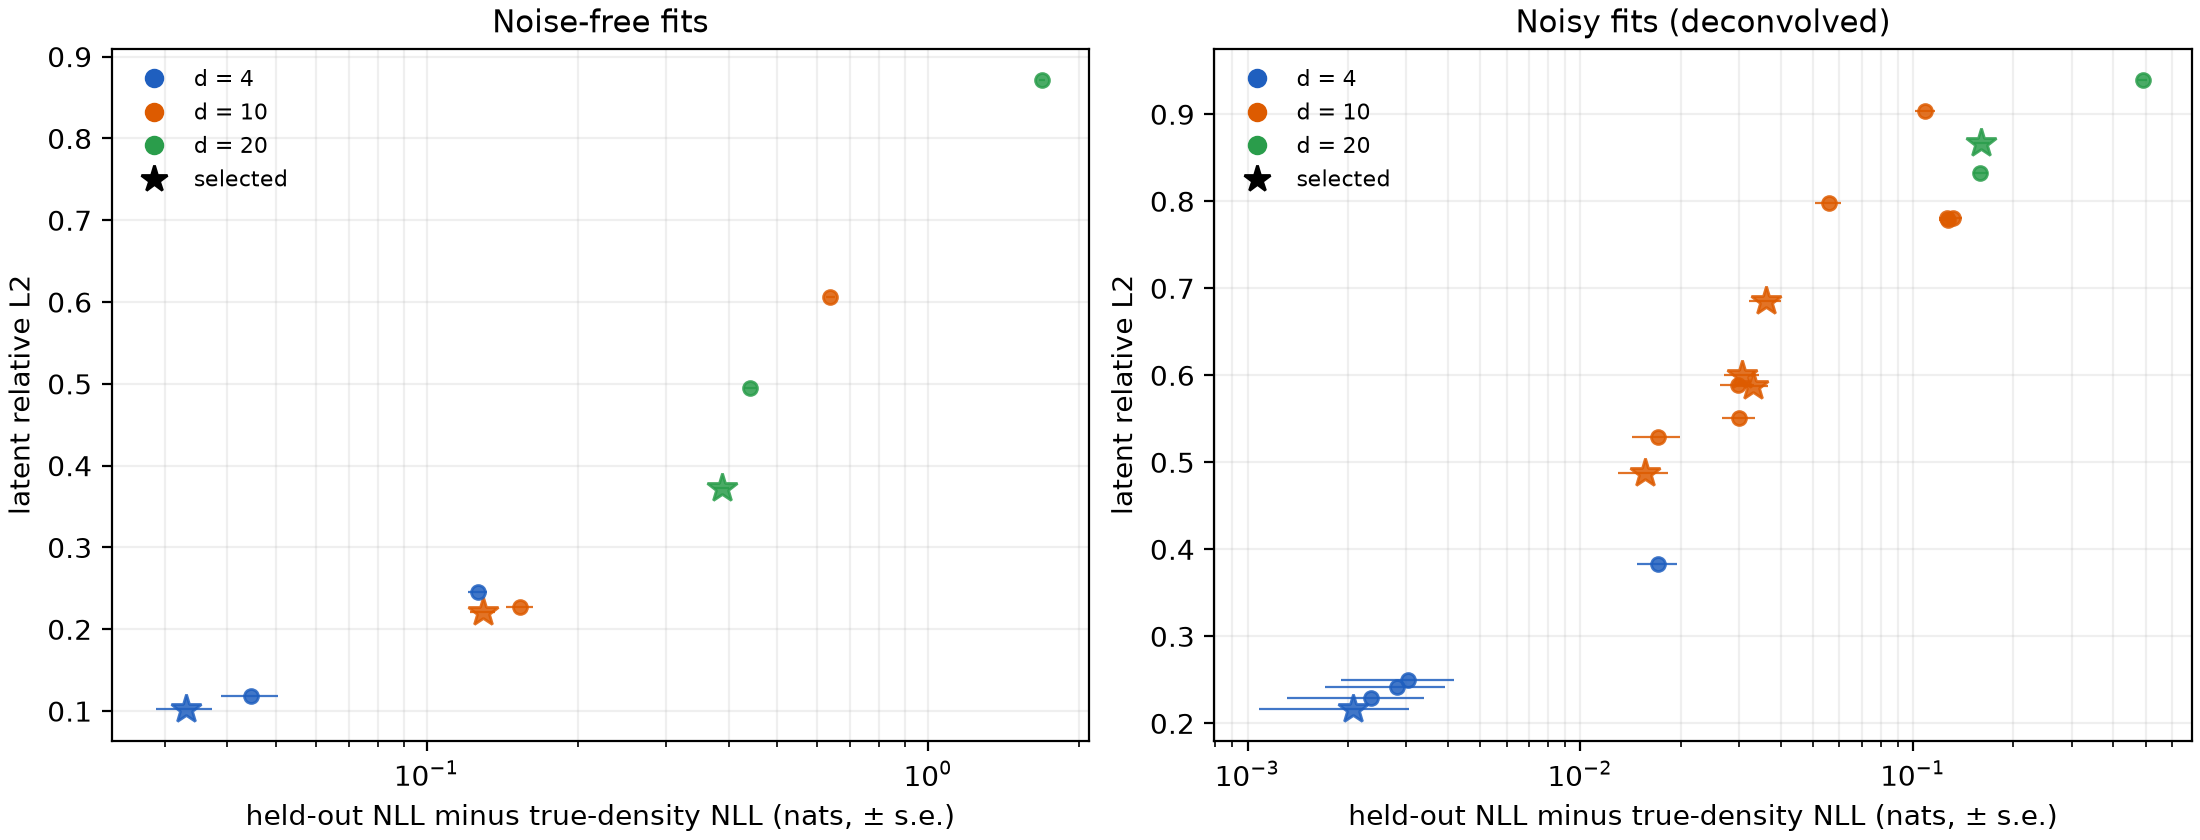
\includegraphics[width=\textwidth]{figures/nll_gap_vs_l2.png}
\caption{Held-out NLL minus the NLL of the true (observation) density against latent $\relLtwo$, for every searched
swirl--pretzel candidate. Stars mark the selected candidates.}
\label{fig:gap}
\end{figure}

\begin{figure}[t]
\centering
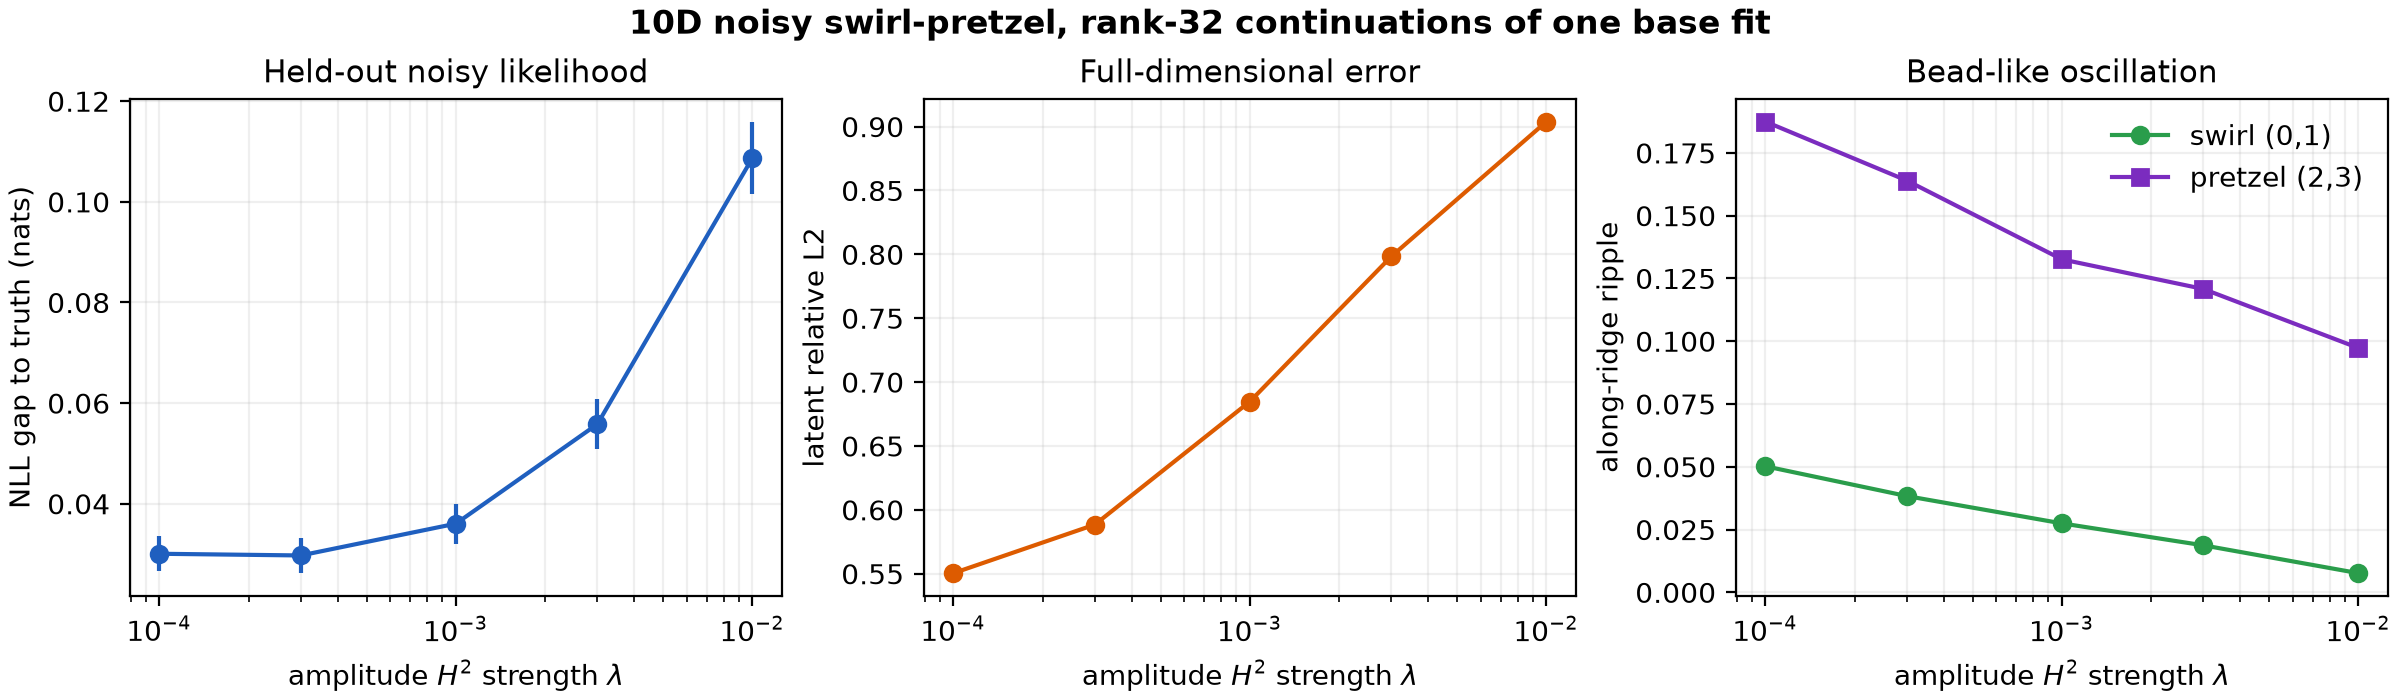
\includegraphics[width=\textwidth]{figures/h2_tradeoff.png}
\caption{Stronger amplitude smoothing in the $d=10$ noisy swirl--pretzel (rank-32 continuations of one base fit):
the ripple falls, while the latent error and the noisy-likelihood gap rise.}
\label{fig:h2}
\end{figure}

%----------------------------------------------------------------------
\subsection{Cryo-EM latent space}
\label{sec:cryo}
The data are RECOVAR~\cite{gilles2025recovar} latent embeddings of a simulated heterogeneous dataset, in 4, 10 and 20
dimensions (separately fitted embeddings), together with per-image posterior covariances. After dropping the 1\% of
images with the largest covariance trace, 99{,}000 remain: 94{,}904 for training and 4{,}096 for validation. Coordinates
are standardized, and plots map back with the Jacobian. The prescribed noise is a 4-component mixture of diagonal
Gaussians obtained by $k$-means clustering of the log per-image variances. It uses only the supplied metadata,
never positions or labels. The current fits come from Algorithm~\ref{alg:hi} continued from earlier
gallery fits: ranks 32 (4D), 64 (10D) and 48 (20D), 49 modes, $H^2$ strength $10^{-4}$ (4D) or $3\cdot10^{-4}$
(10D and 20D), Sobolev preconditioning. Held-out noisy NLLs are 3.531, 9.857 and 24.657.

\begin{figure}[t]
\centering
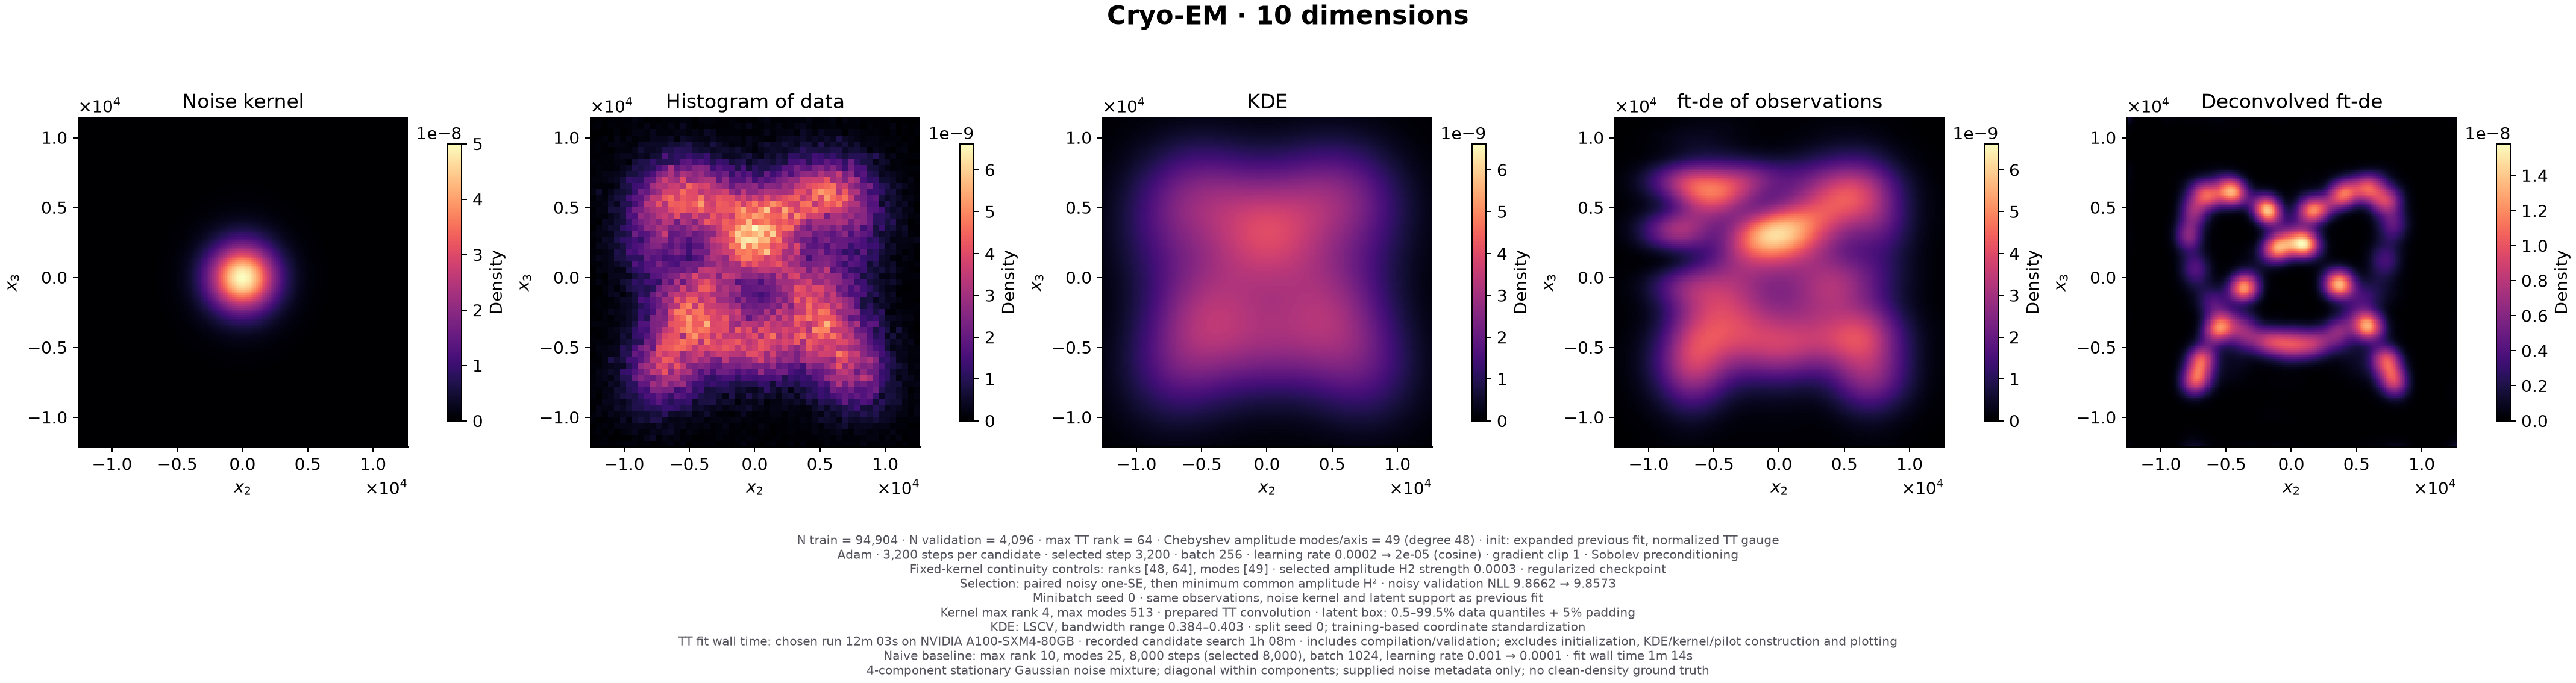
\includegraphics[width=\textwidth]{figures/cryo_d10_23.png}\\
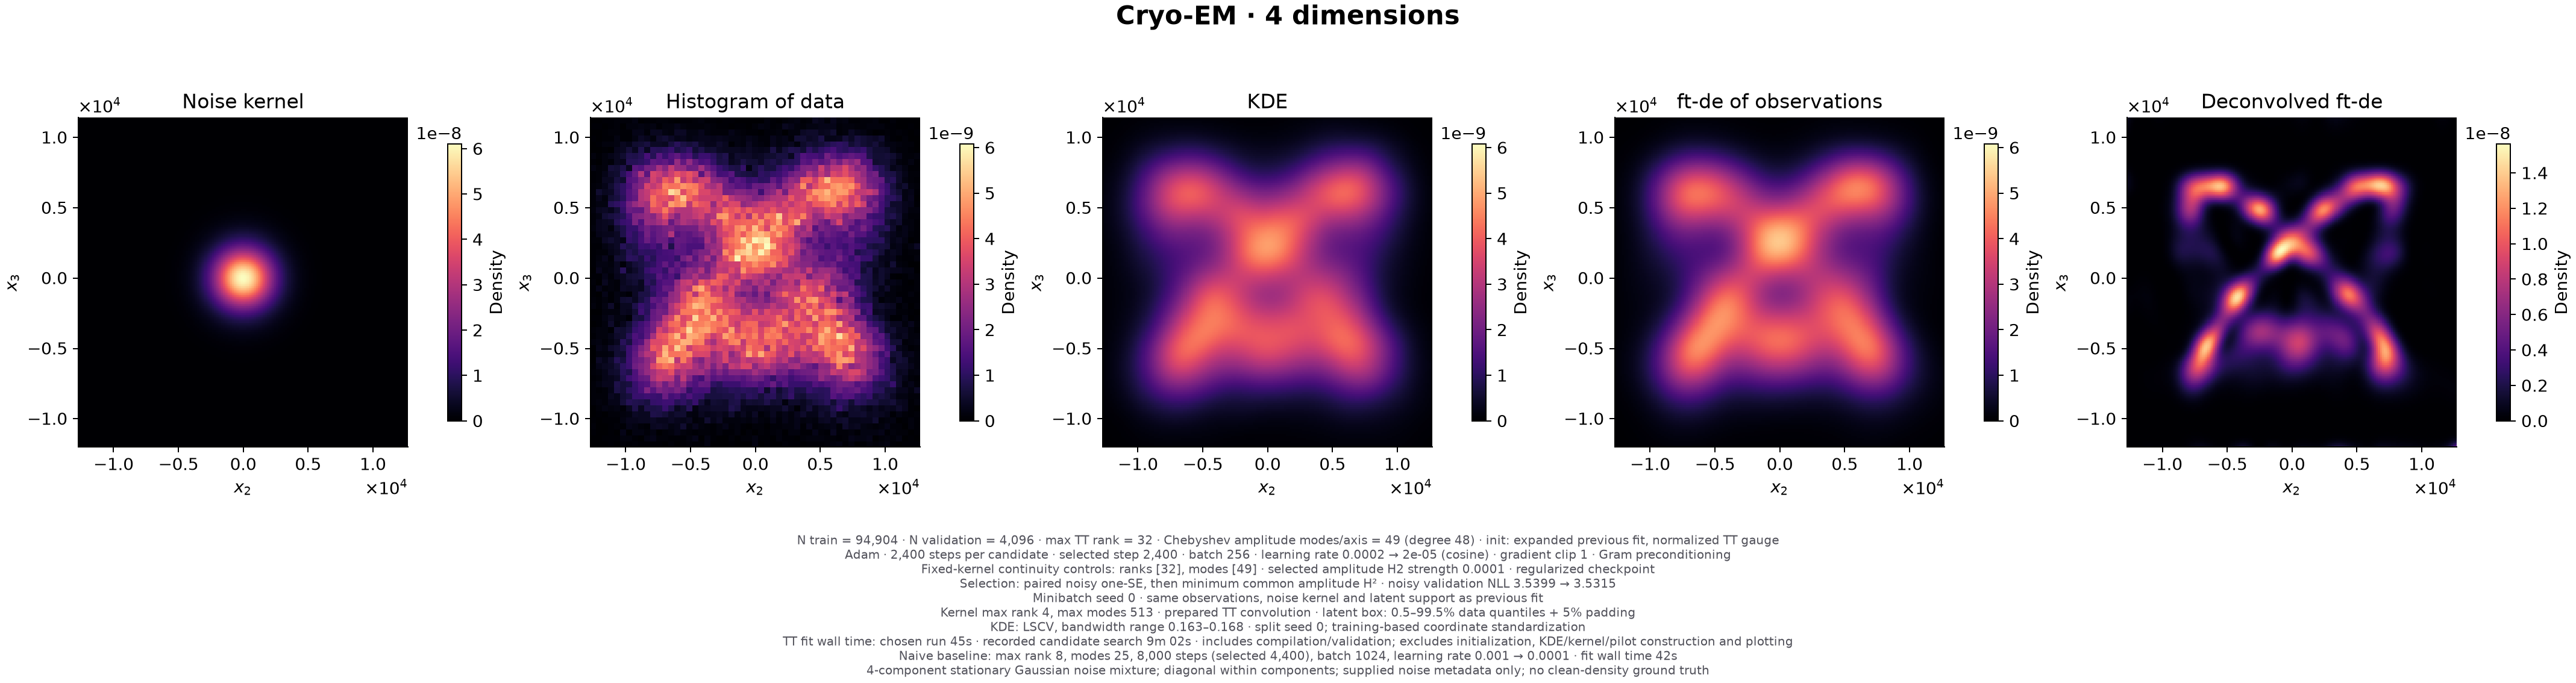
\includegraphics[width=\textwidth]{figures/cryo_d4_23.png}
\caption{Cryo-EM, coordinates $(2,3)$ of the 10D (top) and 4D (bottom) embeddings: supplied noise kernel, data
histogram, KDE, a TT fitted to the observations (no deconvolution), and the deconvolved ft-de.}
\label{fig:cryo}
\end{figure}

\paragraph{Is the clean density beaded?}
The deconvolved marginals in Figure~\ref{fig:cryo} are beaded. The simulation assigns every image to one of
\emph{50 discrete conformational states} (between 20 and about 4{,}900 images each), and these labels can be used, after all fitting, to build
an oracle. For each state we take the mean of its noisy embeddings and the PSD part of
(within-state covariance $-$ mean supplied noise covariance). The oracle clean density is the resulting
50-component Gaussian mixture. We compare it with a \emph{continuous-path counterfactual}: consecutive state
means joined by segments, with interpolated weights and covariances. The oracle convolved with the noise
reproduces the observation-space TT fit to 2D relative $L^2$ between $0.02$ and $0.14$, which validates both the oracle
and the supplied noise model.

\begin{table}[h]
\centering
\begin{tabular}{lccc}
\toprule
embedding & consecutive-state spacing & clean state s.d. & within-state s.d.\\
\midrule
4D  & 1.24 & 0.65 & 1.19\\
10D & 2.16 & 0.43 & 1.08\\
20D & 2.05 & 0.41 & 1.07\\
\bottomrule
\end{tabular}
\caption{Cryo-EM label oracle, in units of the supplied noise standard deviation (medians over states and axes).}
\label{tab:oracle}
\end{table}

\begin{figure}[t]
\centering
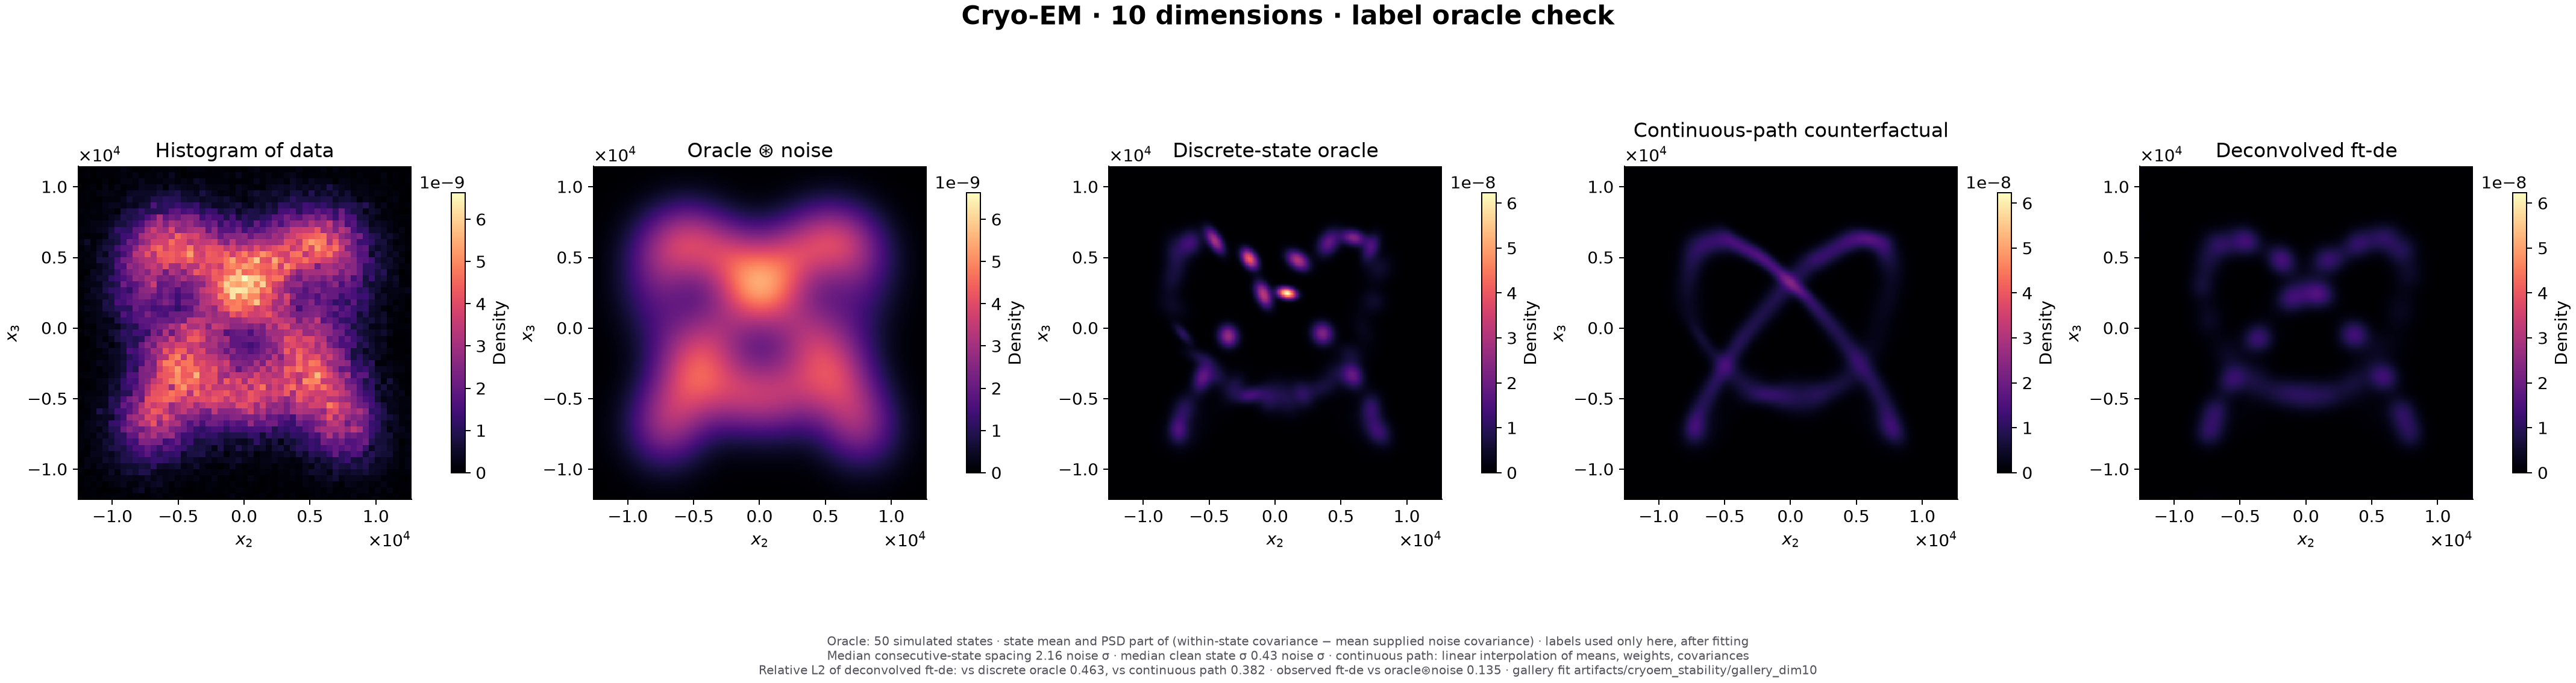
\includegraphics[width=\textwidth]{figures/cryo_oracle_d10_23.png}\\
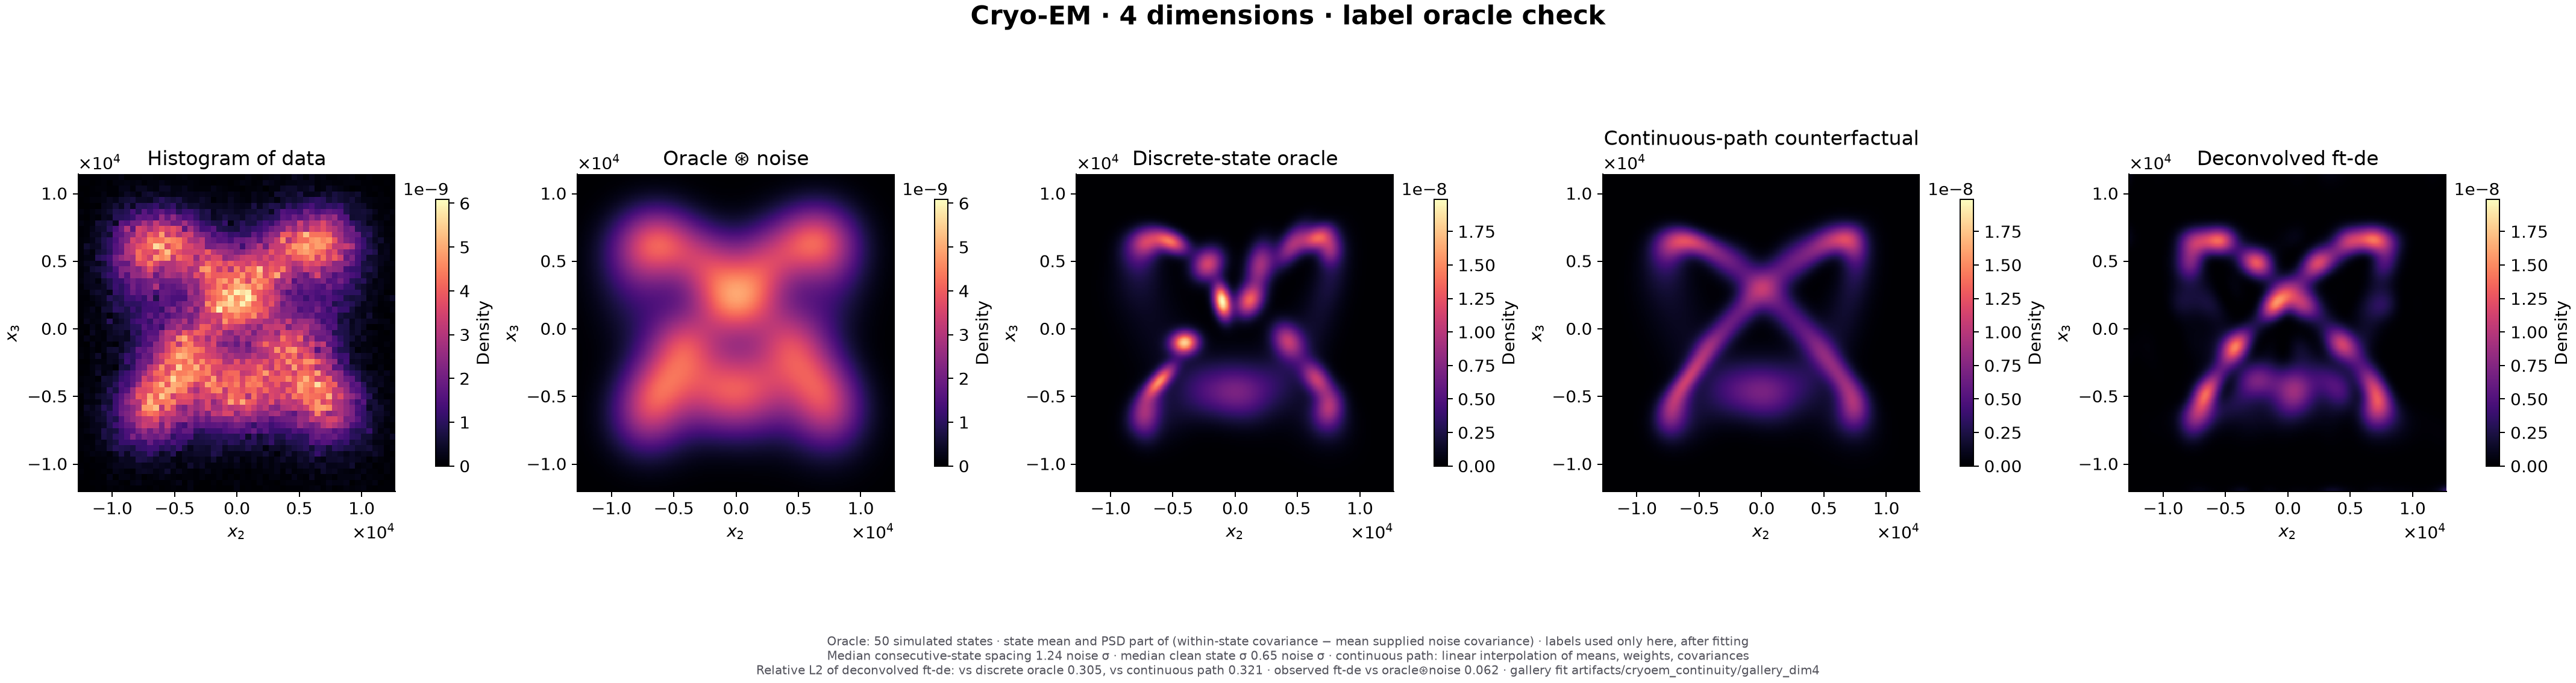
\includegraphics[width=\textwidth]{figures/cryo_oracle_d4_23.png}
\caption{Label oracle for the 10D (top) and 4D (bottom) embeddings: data histogram, oracle $*$ noise, discrete-state
oracle, continuous-path counterfactual, deconvolved ft-de. The last three share a color scale.}
\label{fig:oracle}
\end{figure}

In 10 and 20 dimensions, consecutive states are about five clean-state widths apart (Table~\ref{tab:oracle}), so
the clean density really is a string of separated beads. The noise merges them, which is why histograms and KDEs
look continuous. The deconvolved ft-de reproduces the oracle's qualitative pattern (Figure~\ref{fig:oracle}):
beaded arms, a separate central cluster, and isolated blobs on the lower loops. It does not match individual bead
positions. Its 2D relative $L^2$ is $0.20$--$0.46$ against the discrete oracle and $0.16$--$0.38$ against the
continuous counterfactual, and pointwise $L^2$ heavily penalizes misplaced beads. In the separately fitted 4D
embedding the states are only about two clean widths apart and the oracle is a lumpy but mostly connected ridge. There the
estimate is more beaded than the truth.

The swirl--pretzel experiment gives the other half of the answer. At the same noise-to-width ratio, a continuous
ridge is recovered continuously in 4D, but in 10D the fit fragments it through a detectably suboptimal basin. For
the 10D and 20D cryo-EM fits, both mechanisms are therefore present. The truth is beaded, and the estimator can
also create or move beads. Individual beads should not be read as individual states unless they recur across
independent initializations (Figure~\ref{fig:seeds}); the noisy likelihood alone cannot make this distinction.

%======================================================================
\section{Discussion and open problems}
\label{sec:discussion}
\begin{itemize}[leftmargin=2em,itemsep=2pt]
\item \textbf{What is exact.} Normalization, marginals, smoothness functionals and the convolved likelihood are all exact
contractions. The only numerical approximation is the Chebyshev representation of the prescribed kernel, which is
checked a priori. This removes Monte Carlo deconvolution error entirely, and it makes post-hoc diagnostics exact
when the truth is known.
\item \textbf{Optimization is the bottleneck in higher dimension.} In the swirl--pretzel benchmark the $d=10$ deconvolution
error is associated with a detectable likelihood deficit ($0.016$--$0.03$ nats) that neither continuation, stronger
smoothing nor re-initialization removes. Different initializations land in equally likely basins whose artifacts
differ in location, and averaging their densities cancels part of them without any change in likelihood. Ensembles
over initializations, annealed regularization and rank-adaptive growth are the natural next steps; we have not
established which of them closes the gap.
\item \textbf{Selection.} Noisy held-out NLL ordered the candidates correctly here. However, it is flat at the scale of
the smallest artifacts in $d=4$, and it cannot certify a single fit. Stability across independent initializations
or resamples is a useful complementary diagnostic.
\item \textbf{Rates.} For Gaussian noise the minimax rate is logarithmic~\cite{fan1991optimal}. Our fixed-capacity
estimator does not adapt its rank or degree to $N$. Over $N=10^4$--$3\cdot10^5$ its deconvolution error falls like
$N^{-0.2}$--$N^{-0.25}$, against about $N^{-0.5}$ without noise for GL, and for GL it levels off at the largest $N$
(\S\ref{sec:convergence}). Rank, degree and step budgets that grow with $N$ are needed to tell a statistical floor
from a computational one. A theory for squared low-rank models under supersmooth deconvolution is open.
\item \textbf{Cost.} One convolved likelihood evaluation costs $O(d(r^3sn+r^2s^2n^2))$ per observation. Rank 64 with a
rank-30 kernel is feasible on one GPU, but memory forced gradient accumulation. The noise-free model is
$O(dr^2n)$ per point.
\end{itemize}

\clearpage
\appendix
\section{Code map and reproduction}
\label{app:code}
\begin{center}
\small
\begin{tabular}{p{0.42\textwidth}p{0.53\textwidth}}
\toprule
concept & module / script \\
\midrule
Chebyshev Gram matrices, moments~\eqref{eq:gram} & \texttt{ftde/cheb\_gram.py}\\
squared-TT NLL, $Z$~\eqref{eq:density}--\eqref{eq:nll} & \texttt{ftde/tt\_density.py}\\
exact pair marginals~\eqref{eq:pair} & \texttt{ftde/marginals.py}\\
KDE / LSCV, cross-approximation init & \texttt{ftde/kde.py}, \texttt{ftde/init.py} (chebdGE \texttt{tt\_qtensge})\\
noise TT kernels & \texttt{ftde/noise\_kernel.py}\\
exact convolved likelihood (Prop.~\ref{prop:exact}) & \texttt{ftde/tt\_convolution.py}\\
amplitude Sobolev penalty~\eqref{eq:sobolev} & \texttt{ftde/sobolev.py}\\
Fisher-visibility filter~\eqref{eq:filter}, pilots & \texttt{ftde/fisher\_visibility.py}, \texttt{ftde/marginal\_reference.py}\\
paired one-SE selection & \texttt{ftde/noisy\_model\_selection.py}\\
Algorithm~\ref{alg:gl} & \texttt{scripts/refresh\_density\_fits.py}\\
Algorithm~\ref{alg:hi} & \texttt{scripts/refine\_cryoem\_continuity.py}, \texttt{scripts/swirl\_fits.py}\\
swirl--pretzel truth & \texttt{ftde/swirl.py}; figures \texttt{scripts/swirl\_figures.py}, \texttt{swirl\_ripple.py}\\
cryo-EM label oracle & \texttt{scripts/audit\_cryoem\_oracle.py}\\
sample-size sweep & \texttt{scripts/run\_convergence\_sweep.py}, \texttt{scripts/convergence\_summary.py}\\
figures of this note & \texttt{scripts/note\_figures.py}\\
\bottomrule
\end{tabular}
\end{center}
Run commands from the repository root in the \texttt{chebdGE} environment, inside one GPU allocation (\texttt{salloc}, then
\texttt{srun} per step), for example
\texttt{python scripts/swirl\_fits.py -{}-dim 10 -{}-noise mixture -{}-output artifacts/swirl/swirl\_mixture\_dim10}.
Completed candidates are reused, and runs refuse to overwrite a directory whose settings differ.
See \texttt{docs/swirl\_benchmark.md} and \texttt{docs/figure\_refresh.md} for full settings.


\bibliographystyle{abbrvnat}
\bibliography{citations}

\end{document}
